\documentclass[a4paper,11pt,oneside]{report}

% --- Preamble - Essential Packages and Configurations ---
\usepackage[colorlinks=true, linkcolor=black, citecolor=black, filecolor=black, urlcolor=blue]{hyperref}
% Language setup
\usepackage[utf8]{inputenc} % For direct UTF-8 input
\usepackage[T1]{fontenc}    % For proper font encoding (better hyphenation, special characters)
\usepackage[french, english]{babel} % Order matters: last one loaded is active. If your document is primarily English, put english last. If primarily French, put French last.

% Font package
\usepackage{palatino} % Palatino font

% Graphics and figures
\usepackage{graphicx} % For including images
\usepackage{float}    % For the [H] placement specifier, good for strict figure placement
\usepackage{subfig} % Recommended replacement for ubfigure, if you intend to use sub-figures.

% Math and Symbols
\usepackage{amsmath}    % For advanced math environments
\usepackage{amssymb}    % For additional math symbols
\usepackage{latexsym}  % For some LaTeX symbols

% Tables
\usepackage{array}      % For extended column definitions in tables
\usepackage{booktabs}  % For professional looking tables (toprule, midrule, bottomrule)
\usepackage{multirow}  % For cells reaanning multiple rows in tables
\usepackage{longtable} % For tables spanning multiple pages
\usepackage{tabularx}

% Links and References
\usepackage{url}        % For better URL handling
\def\UrlBreaks{\do\/\do-} % Allows URL to break at / and -
\usepackage{breakurl}    % Allows breaking long URLs
\usepackage[hidelinks]{hyperref} % For clickable links, hidelinks removes colored boxes

% Glossary and Acronyms
\usepackage[acronym]{glossaries} % For glossaries and acronyms
\makeglossaries             % Command to make glossaries

% Bibliography
\usepackage[backend=biber, style=authoryear]{biblatex} % Modern bibliography management
\addbibresource{refs.bib} % Your bibliography file

% Document Structure and Formatting
\usepackage{setspace}    % For adjusting line spacing
\linespread{1.1}         % Sets overall line spacing to 1.5 (double spacing)
\usepackage{titlesec}    % For customizing sectioning titles
\usepackage{verbatim}    % For commenting out blocks of text
\usepackage{enumitem}    % For customizing lists (itemize, enumerate)
\usepackage{pifont}      % For special symbols like dingbats (e.g., \ding{...})
\usepackage{lettrine}    % For dropped capitals (initials)

% Use the correct fancyhdr package
\usepackage{fancyhdr}
\usepackage{nccrules}

% Page layout settings
% NOTE: The geometry package is recommended for page layout.
% The manual settings below may cause unexpected issues.
\setlength{\doublerulesep}{\arrayrulewidth} % For tables
\setlength{\textwidth}{16cm}
\setlength{\textheight}{24cm}
\setlength{\marginparwidth}{-4cm} % This seems unusual, usually positive value or zero
\setlength{\evensidemargin}{-4cm}  % This also seems unusual, might cause issues
\setlength{\hoffset}{-1.7cm}
\setlength{\voffset}{-1cm}
\setlength{\topmargin}{-0.5cm}
\setlength{\footskip}{27pt}
\addtolength{\headsep}{10pt}

% Section numbering depth - FIX for \subsubsection not displaying as title
\setcounter{secnumdepth}{3} % Number subsections up to subsubsection level
\setcounter{tocdepth}{3}    % Include subsections up to subsubsection in ToC

% User-defined command for contact link
\newcommand{\contactlink}{\textsuperscript{\hyperref[biblio]{\P}}} % Corrected \P symbol

% --- CUSTOM COMMANDS FROM YOUR FRIEND'S EXAMPLE ---

% Chapter title on its own page
\makeatletter
\renewcommand\@makechapterhead[1]{%
  \thispagestyle{plain}%
  \vspace*{\fill}%
  \begin{center}%
    \Huge\bfseries Chapter \thechapter\ :\par%
    \vspace{1em}%
    \Huge\bfseries #1\par%
  \end{center}%
  \vspace*{\fill}%
  \clearpage
}
\renewcommand{\chaptermark}[1]{\markboth{Chapter \thechapter\ : #1}{}}
\renewcommand{\sectionmark}[1]{}
\makeatother

% Header and Footer Style
\fancypagestyle{mymain}{%
  \fancyhf{}%
  \renewcommand{\headrulewidth}{1pt}%
  \fancyhead[R]{\small\nouppercase{\leftmark}}%
  \fancyfoot[C]{\thepage}%
}
\pagestyle{mymain}

% --- End of Preamble ---

\begin{document}

%----------------------------------------------------------------------------
%   Page de garde
%----------------------------------------------------------------------------
\thispagestyle{empty}
%\input{Pages/First_Pages/garde.tex} % Commented out as in your original

\pagenumbering{roman}
\setcounter{page}{1}
\newpage
\thispagestyle{empty}
%\input{Pages/First_Pages/signature.tex} % Commented out as in your original
\thispagestyle{empty}
\input{Pages/First_Pages/abstract.tex}
\thispagestyle{empty}
\begin{spacing}{1.3}
\centerline{\emph{\LARGE{Acknowledgments }}}

\vspace*{1cm}
\emph{
\lettrine[lines=2]{I}\\t is with great respect and profound gratitude that I extend my heartfelt thanks to all those who, directly or indirectly, contributed to the successful completion of this project. Your support, presence, encouragement, and invaluable guidance have been instrumental to our achievement, making this journey both enriching and unforgettable.
\newline \newline \indent First and foremost, I would like to express my sincere appreciation to Mr. Taoufik Ladhari, my academic supervisor, and Mr. Fawzi Msahli, my co-supervisor. The privilege of being guided by their expertise throughout this project has been invaluable. Their unwavering support, insightful feedback, and constant encouragement were instrumental to my progress, shaping not only this work but also my understanding of the field.
\newline \newline \indent I am equally grateful to Mr. Saddem Ben Salah, my industrial supervisor, for welcoming me to XPERT-MECA and offering me the opportunity to carry out my internship in such a dynamic and professional environment. His technical guidance, mentorship, and trust significantly enriched my practical knowledge and deepened my understanding of the industrial world. 
\newline \newline \indent Also, I want to convey my utmost respect and gratitude to the esteemed members of the jury for the honor they have bestowed upon me by examining and evaluating this modest contribution. I hope that this work meets their esteemed standards and expectations. \\
\newline  \newline \indent Finally I dedicate this work to my beloved parents, whose boundless love, countless sacrifices, and unwavering support have been the very foundation of my journey and success.This achievement is not mine alone; it belongs to you both. It is a reflection of your sacrifices, your dreams for me, and the endless support you have given without asking for anything in return.}

\end{spacing}
\newpage


%----------------------------------------------------------------------------
%   La tables des matieres, des figures et la liste des tableaux
%----------------------------------------------------------------------------
\begin{spacing}{1.3}
\tableofcontents
\end{spacing}
\newpage
\newpage
\begin{spacing}{1.5}
\listoffigures
\end{spacing}
\newpage
\newpage
\begin{spacing}{1.5}
\listoftables
\end{spacing}
\newpage
\newpage
\pagestyle{plain}
\section*{\Huge List of Abbreviations}
\vspace{1cm}
\begin{description}
\item[\textbf{SAV:}] After-Sales Service
\item[\textbf{CNC:}] Computer Numerical Control
\item[\textbf{PLC:}] Programmable Logic Controller
\item[\textbf{TIA:}] Totally Integrated Automation
\item[\textbf{IDE:}] Integrated Development Environment
\item[\textbf{HMI:}] Human-Machine Interface
\item[\textbf{GRAFCET:}] Graph for Step-by-Step Control
\item[\textbf{I/O:}] Input/Output
\item[\textbf{LAD:}] Ladder Diagram
\item[\textbf{FBD:}] Function Block Diagram
\item[\textbf{SCL:}] Structured Control Language
\item[\textbf{STL:}] Statement List
\item[\textbf{SFC:}] Sequential Function Chart
\item[\textbf{DBs:}] Data Blocks
\item[\textbf{PTRIG:}] Single-Shot Pulse
\item[\textbf{FRL:}] Filter, Regulator, Lubricator
\item[\textbf{MES:}] Manufacturing Execution System
\end{description}
\newpage
%---- General Introduction
\pagenumbering{arabic} % Start arabic numbering for main content
\begin{spacing}{1.3}

\chapter*{General Introduction  
%\markboth {Introduction }{}}
\markboth {General Introduction}{}}
\addcontentsline{toc}{chapter}{General Introduction}



% \lettrine[lines=2]{T}\\he automobile business is continually developing, fueled by technology advancements that are redefining cars. From engine control and advanced driver assistance systems, to infotainment systems, software is crucial in regulating the different components of a vehicle's operation. Nowadays automotive software engineering has gained at least as much attention and importance as any other engineering aspect of the automotive industry process.
% \newline
% \newline
% \indent
% With the modern era of interconnected systems and high-speed communication, the automotive industry had also merged the lines of this technological advancement. The vehicle of the future is getting shipped with advanced driver assistance systems (ADAS), connected vehicles, over-the-air (OTA) update, autonomous driving and recently with the shift towards electric vehicles (EVs) that further amplifies the importance of software, as it orchestrates battery management, energy efficiency, and charging infrastructure integration. With this increase of complexity and the need for precision as well as real time operations, these systems rely on accurate timing information for various functioning. Thus the need for precise time synchronization has become paramount and the demand for such a module has grown significantly.



\newacronym{adas}{ADAS}{Advanced Driver Assistance Systems}
\newacronym{evs}{EVs}{Electric Vehicles}
\newacronym{ota}{OTA}{Over-the-air}
\newacronym{v2x}{V2X}{Vehicle to Everything}
\newacronym{ecus}{ECUs}{Electronic Control Units}
\newacronym{ptp}{PTP}{Precision Time Protocol}
\newacronym{ieee}{IEEE}{Institute of Electrical and Electronics Engineers}


\lettrine[lines=2]{I}\\n the contemporary industrial landscape, characterized by fast-paced technological advancements and heightened market demands, automation and robotics have emerged as fundamental drivers of innovation and productivity. These technologies revolutionize manufacturing processes by enhancing precision, reliability, and speed while minimizing human error and operational costs. The integration of automated systems not only streamlines production but also empowers industries to adapt swiftly to changing requirements, thus maintaining a competitive edge in the global marketplace.


Against this backdrop, the present final year project was conducted within the premises of Xpert-Meca, a dynamic company renowned for its expertise in the design, development, and implementation of tailor-made automated and robotic solutions. Xpert-Meca’s commitment to advancing industrial automation makes it an ideal environment for undertaking projects that combine theoretical knowledge with practical application.


The project’s core objective was to conceive, develop, and simulate an automated cube-sorting cell. This system was specifically designed to demonstrate the potential and versatility of modern automation technologies in an industrial context, particularly as an exhibit for trade fairs and industrial exhibitions. The sorting cell not only illustrates the synergy between robotics and automation control but also serves as a practical showcase of how complex processes can be managed efficiently through integrated systems.

The work was systematically organized into four comprehensive chapters, each addressing distinct but interconnected aspects of the project:


\begin{itemize}
\item \textbf{Chapter 1} introduces the host company, Xpert-Meca, providing insight into its organizational structure, areas of expertise, and external collaborations. This chapter also outlines the complete project framework, including the problem statement, objectives, the chosen solution, and the high-level operating principle of the automated sorting cell;
\item \textbf{Chapter 2} details the system's design and architecture, covering the hardware and software components. It provides a technical overview of the operative parts (KUKA robot, conveyors, pneumatic systems, and sensors), the control parts (PLC, HMI, and robot controller), and the supporting electrical and pneumatic cabinets. This chapter also outlines the software tools used for control, programming, design, and visualization;
\item \textbf{Chapter 3} delves into the control system and automation of the robotic sorting cell, detailing its automation logic and programming. It explains how a Programmable Logic Controller (PLC) serves as the system's central brain, prioritizing safety and sequential operation. The chapter also covers the use of the GRAFCET graphical language for designing the control logic, and the TIA Portal software for a unified engineering framework that integrates hardware configuration, PLC programming, and HMI design. Finally, it details the PLC programming implementation, including hardware configuration, I/O and tag management, and the use of various programming languages like Ladder Diagram (LAD) and fundamental programming blocks;
\item \textbf{Chapter 4}  delves into the system integration and verification of the automated sorting cell. It details the PROFINET communication framework used to connect the PLC, robot, and other components via a central router. The chapter also explains the crucial role of virtual commissioning by demonstrating how software like TIA Portal and Blender were used to create a "digital twin." This allowed for comprehensive simulation and verification of the control logic, HMI functionality, and mechanical movements, ensuring a robust and reliable design before physical implementation.

\end{itemize}

Throughout the project, I tackled significant technical challenges, from initial design constraints and component compatibility to programming and system integration hurdles. The solutions I developed combine analytical thinking with practical engineering skills and adherence to best industry practices. Ultimately, this endeavor provided a valuable learning experience, bridging academic knowledge with industry requirements and offering a solid foundation for future work in industrial automation and robotics.
\end{spacing}
\newpage


%----chapter1 Overview
\chapter{Company Overview and General Project Framework}

\section{Introduction}
In an ever-evolving industrial context, companies are constantly seeking to enhance their performance through automation, robotics, and technological innovation. My final year project aligns with this trend and was carried out at Xpert-Meca, a company specialized in robot integration and the design and manufacturing of special-purpose machines.

This first chapter aims to present the overall context of the project, starting with a description of the host company, its activities, clients, and partners. It then transitions to a general presentation of the project, including its objectives and high-level operating principles, providing a solid foundation for the detailed technical information presented in subsequent chapters.

\section{Company Presentation}
\subsection{Introduction}
Founded in 2014 by a team of engineers experienced in mechanics, automation, and robotics, Xpert-Meca is an official partner of KUKA Robots. The company specializes in the integration and servicing of KUKA robots in Tunisia and North Africa, the design and production of special-purpose machines using numerical simulation, as well as industrial maintenance. Situated at Street Khaznadar in Hammam-Sousse, Sousse, Tunisia, the company's strategic placement facilitates access to key industrial networks and a skilled local workforce. Xpert-Meca provides complete and customized technical solutions for robots used in handling, welding, cutting, laser processing, polishing, packaging, and palletizing\hyperref[sec:bibliography]{[1]}.

The company adapts to its clients' products and production processes to design and deliver turnkey robotic solutions. The grippers, bases, conveyors, and all surrounding mechanical equipment are fully designed and manufactured by its in-house design office. The logos of Xpert-Meca and its official partner, KUKA, are shown in Figure \ref{fig:XPERT-MECA}.

\begin{figure}[H]
\centering

\includegraphics[width=0.6\textwidth]{Images/Chap1/KukaNxpert.png}
\caption[XPERT-MECA Logo and KUKA Logo]{XPERT-MECA Logo and KUKA Logo }
\label{fig:XPERT-MECA}
\end{figure}

\section{Xpert-Meca's Core Teams and Operations}
\subsection{Mechanical and Automation Development Team}

The mechanical development team includes experienced engineers and technicians responsible for designing and modeling mechanical components. Their expertise enables the creation of robust, precise, and reliable machines tailored to client needs. The automation team designs and programs control systems for the solutions. These professionals master the latest technologies and programming languages, ensuring smooth machine and process operation. A photo of the development teams is shown in Figure \ref{fig:XPERT-MECA_DevTeam}.

\begin{figure}[H]
\centering
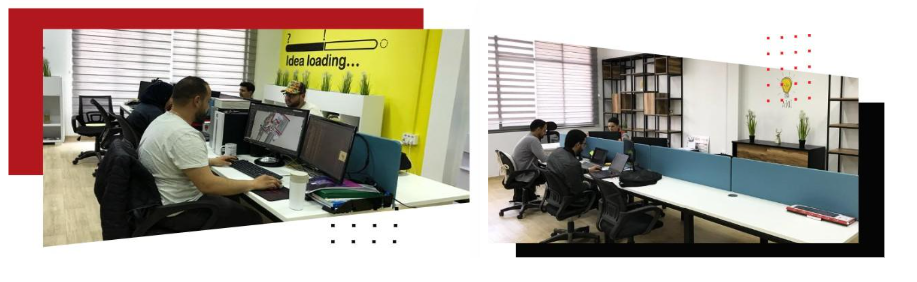
\includegraphics[width=1\textwidth]{Images/Chap1/DevTeam.png}
\caption[Mechanical Dev. Team and Automation Dev. Team]{Mechanical Dev. Team and Automation Dev. Team }
\label{fig:XPERT-MECA_DevTeam}
\end{figure}

\subsection{Robotics Team}
This team specializes in the integration and programming of industrial robots, which are central to Xpert-Meca’s core business. They are responsible for a full range of tasks, from the initial setup and calibration of robotic arms to the development of complex motion programs for diverse applications such as welding, handling, and palletizing. By working closely with clients, they develop custom robotic solutions that are meticulously designed to optimize production efficiency, ensure high precision, and enhance overall productivity. The team's expertise is critical to translating a client’s needs into a fully functional, automated robotic process, as shown in Figure \ref{fig:XPERT-MECA_Robotics}.

\begin{figure}[H]
\centering
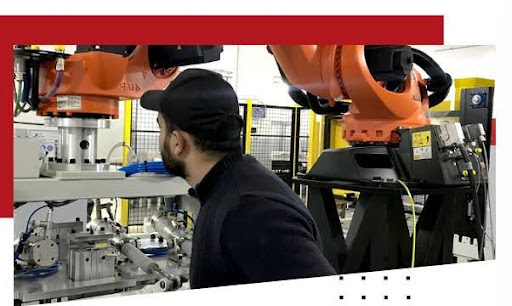
\includegraphics[width=0.6\textwidth]{Images/Chap1/RoboticTeam.jpg}
\caption[ Robotics team area]{ Robotics team area}
\label{fig:XPERT-MECA_Robotics}
\end{figure}

\subsection{Assembly Team}
The assembly team is responsible for the crucial final stage of system construction. They ensure that all designed and manufactured components—including mechanical structures, electrical panels, and pneumatic systems—are precisely and correctly assembled. Their work involves the meticulous installation and wiring of machines and systems according to detailed engineering plans. This team plays a vital role in verifying the physical integrity of the final product and ensuring that the mechanical and electrical installations are robust and perform optimally before the system is commissioned. The assembly zone is shown in Figure \ref{fig:XPERT-MECA_Assembly}.

\begin{figure}[H]
\centering
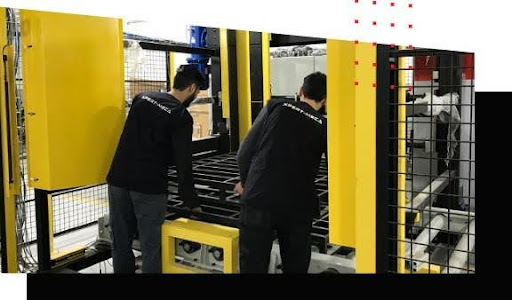
\includegraphics[width=0.6\textwidth]{Images/Chap1/AssemblyTeam.jpg}
\caption[ Assembly zone]{ Assembly zone}
\label{fig:XPERT-MECA_Assembly}
\end{figure}

\subsection{Machining Team}
This team is composed of skilled technicians who are experts in the production of high-precision mechanical parts. They operate a variety of advanced machinery, including CNC (Computer Numerical Control) machines, lathes, and milling machines, to fabricate custom components. The team’s work is essential for producing the specialized parts required for grippers, fixtures, and other bespoke equipment. Their expertise ensures that every component meets stringent quality and dimensional standards, which is fundamental to the reliability and performance of Xpert-Meca’s final products. The machining area is shown in Figure \ref{fig:XPERT-MECA_Machining}.

\begin{figure}[H]
\centering
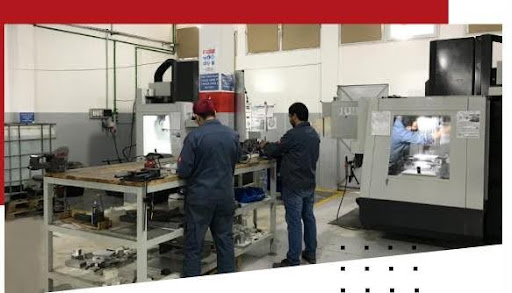
\includegraphics[width=0.6\textwidth]{Images/Chap1/MachiningTeam.jpg}
\caption[ Machining area]{Machining area}
\label{fig:XPERT-MECA_Machining}
\end{figure}

\subsection{Sales Team}
The sales team is the primary interface between Xpert-Meca and its clients. Their main focus is on customer satisfaction, providing support from the initial consultation through to the final purchase. The team is responsible for understanding client needs, offering tailored technical and commercial advice, and presenting solutions that align with the client’s operational and financial goals. They play a key role in building and maintaining strong customer relationships, which is vital for the company’s growth and market presence. The commercial area is shown in Figure \ref{fig:XPERT-MECA_Sales}.

\begin{figure}[H]
\centering
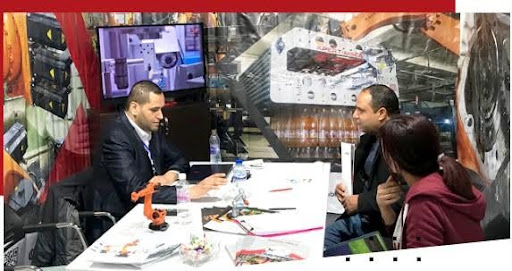
\includegraphics[width=0.6\textwidth]{Images/Chap1/Sales.jpg}
\caption[ Commercial area]{Commercial area}
\label{fig:XPERT-MECA_Sales}

\end{figure}

\subsection{After-Sales Service (SAV) Team}
Dedicated to ensuring the long-term operational continuity of installed systems, the After-Sales Service (SAV) team provides technical support and maintenance. Their role is to respond to client requests, troubleshoot issues, and perform routine maintenance to prevent system failures. This team’s effective and rapid response ensures that any downtime is minimized and that the installed solutions continue to operate reliably. Their work is crucial for upholding the company's reputation for quality and support. The after-sales service zone is shown in Figure \ref{fig:XPERT-MECA_AfterSales}.

\begin{figure}[H]
\centering
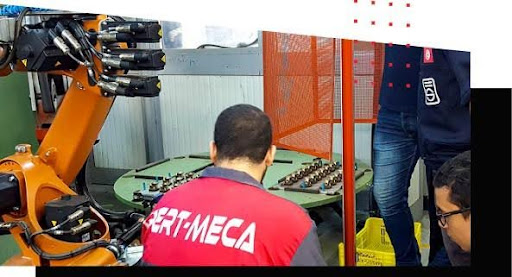
\includegraphics[width=0.6\textwidth]{Images/Chap1/AfterSales.jpg}
\caption[ After-sales service zone]{After-sales service zone}
\label{fig:XPERT-MECA_AfterSales}
\end{figure}

\subsection{Procurement Team}
This team is responsible for the strategic management of the supply chain, from sourcing materials to inventory management. They handle the procurement of all necessary components and materials for production, including electronic parts, mechanical components, and raw materials. The team carefully selects and vets suppliers to ensure that all resources meet quality standards and are available in a timely manner. Their efficient management of the supply process is critical for maintaining smooth manufacturing operations and controlling project costs. Figure \ref{fig:XPERT-MECA_Procurement} provides a look at the procurement and storage area.

\begin{figure}[H]
\centering
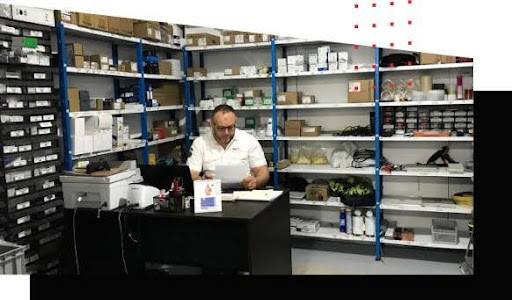
\includegraphics[width=0.6\textwidth]{Images/Chap1/Procurement.jpg}
\caption[Procurement and storage area]{ Procurement and storage area}
\label{fig:XPERT-MECA_Procurement}
\end{figure}
\section{External Ecosystem and Collaborations}
\subsection{Business Sectors}
Xpert-Meca extends its expertise in robotics and automation across a diverse range of industrial sectors, providing tailored solutions that address the specific needs of each market. The company’s strategic focus on these key industries allows for the development of highly specialized applications that enhance productivity, quality, and safety.

\begin{itemize}
\item \textbf{Agro-food Sector}: In this industry, Xpert-Meca focuses on automating processes that require precision and hygiene, such as handling, packaging, and sorting. Robotic solutions are employed to increase throughput and ensure consistency in food production lines;
\item \textbf{Automotive Sector}: This is a core area for the company, where robust robotic applications are essential. Xpert-Meca provides advanced solutions for critical tasks like robotic welding, material handling, assembly, and quality inspection, leveraging the precision of KUKA robots;
\item \textbf{General Industrial Sector}: The company offers customized automation solutions for a broad range of general manufacturing and assembly applications. This includes the design and production of special-purpose machines for specific client requirements, optimizing various stages of the manufacturing process;
\item \textbf{Educational Sector}: In collaboration with academic institutions and technical training centers, Xpert-Meca supplies educational robotic platforms and provides specialized training. This helps prepare future engineers and technicians for modern industrial environments by giving them hands-on experience with advanced robotics and automation systems.
\end{itemize}

\subsection{Clients}
Xpert-Meca’s clients include companies from various industrial domains, ranging from local manufacturers to multinational groups seeking innovative robotic and automation solutions. The logos of some of Xpert-Meca's key clients are presented in Figure \ref{fig:ClientsLogos}.

    \begin{figure}[H]
    \centering
    
\includegraphics[width=1\textwidth]{Images/Chap1/ClientsLogos.jpg}
    \caption[ Clients Logos ]{ Clients Logos }
    \label{fig:ClientsLogos}
    \end{figure}

\subsection{Partners}
The official partners of Xpert-Meca are:

\begin{itemize}
    \item \textbf{KUKA}, a global automation corporation, is a leading provider of intelligent automation solutions. Founded in Augsburg, Germany, in 1898 by Johann Josef Keller and Jakob Knappich, the company's name is an abbreviation of "Keller und Knappich Augsburg". Since its inception, KUKA has been at the forefront of technological innovation, expanding its offerings from initial products like acetylene gas lighting to a wide range of industrial applications today;
    
    KUKA provides everything from industrial robots and software to fully automated production systems and their connectivity. The company serves various markets, including automotive (with a focus on e-mobility), electronics, metal and plastic, consumer goods, e-commerce, and healthcare. As of 2024, KUKA has approximately 15,000 employees and operates in more than 50 countries with over 100 locations.
    
    
    \item \textbf{Optimal Business Growth (OBG)} is a company based in Tunisia that offers digital transformation services to businesses, particularly in the field of IT and digitalization. They focus on assisting companies in optimizing their productivity, improving their efficiency, and increasing their profitability through technology\hyperref[sec:bibliography]{[2]}.
\end{itemize}

    
\section{Project Framework}
This section provides a comprehensive overview of the project's foundation, from the initial problem to the final solution. It details the core objectives and the principles guiding the development of the automated sorting cell.
\subsection{Problem Statement}
In the context of technology fairs and industrial exhibitions, there is a clear need for demonstrations that are not only dynamic and visually appealing, but also educational. The challenge is to create an engaging showcase that effectively highlights the core principles of Industry 4.0, such as robotics and automation, in a way that is easily accessible and understandable to a broad audience. This project addresses this need by developing an inspiring, interactive demonstration that leverages modern automation principles to spark visitor interest and engagement.

\subsection{Project Objective}
The main goal of this project is to design and implement an interactive and visual demonstration system that serves as a powerful showcase for advanced industrial technologies. The system must be developed to be showcased at industrial fairs or tech events, with the following key objectives:
\begin{itemize}
\item \textbf{Showcase Robotics Capabilities:} Highlight the precision, speed, and reliability of industrial robots in a dynamic and safe environment;
\item \textbf{Illustrate System Integration:} Clearly demonstrate the seamless coordination and communication between various subsystems, including robots, vision systems, and conveyors;
\item \textbf{Engage and Educate the Audience:} Capture visitors' attention through a smooth, colorful, and highly visual demonstration, while making the underlying principles of automation easy to understand;
\item \textbf{Validate the Full Development Cycle:} Prove the project's success by executing the full engineering process, from initial design and part selection to the final implementation and automation of the solution.
\end{itemize}

\subsection{Project Solution and Operating Principle}
To address the need for a dynamic and educational demonstration, the project solution is the design and implementation of a fully automated cube handling and sorting cell. This cell serves as a sophisticated showcase of modern industrial automation and robotics principles.
\newline
The system's core is the KUKA KR AGILUS industrial robot, which performs precise pick-and-place operations. Cubes of various colors are fed into the system via two motorized belt conveyors. Their presence is detected by sensors, while a vision system powered by a Raspberry Pi and a camera identifies the color of each cube. The robot then retrieves the cubes and sorts them into their designated bins based on the color detected.

The entire process is automated and runs in a continuous loop, which makes it ideal for uninterrupted demonstrations at industrial exhibitions. The system's operation is governed by a repetitive, automated, and visual cycle:

\begin{itemize}
\item \textbf{Cube Transportation:} Cubes of different colors are transported by motorized conveyors;
\item \textbf{Presence Detection:} Their presence is detected by a series of sensors, which signal the system to begin the next phase;
\item \textbf{Color Analysis:} An industrial camera, placed strategically, analyzes the color of the cube;
\item \textbf{Robotic Sorting:} The KUKA robot picks up the cubes with a custom gripper and places them into dedicated bins based on the detected color;
\item \textbf{Cycle Restart:} Once sorted, the cubes are recirculated back onto the conveyor to restart the cycle continuously.
\end{itemize}

The entire system's logic and sequencing are managed by a Siemens PLC, while an HMI provides real-time feedback and control, ensuring the system is both functional and transparent for any audience.

\subsection{System Flowchart}
To provide a clear, high-level overview of the system's operational flow, the diagram in annex \ref{fig:Flowchart} illustrates the sorting cell's general behavior from initialization to cube classification. It simplifies the cycle into key actions and shows how the different components interact in a sequential manner.



\subsection{Added Value}
The robotic sorting cell is designed not only as a functional system but also as a strategic tool for showcasing advanced technology. Its core value proposition can be broken down into the following key benefits:

\begin{itemize}
\item \textbf{Interactivity}: The system's precise and fluid movements, combined with the visual appeal of sorting colorful objects, naturally captures and holds the attention of visitors. This dynamic behavior transforms a passive observation into an active viewing experience, making it a compelling centerpiece for any exhibition booth. This interactivity is key to generating interest and engaging potential clients and students;

\item \textbf{Educational aspect}: The demonstration provides a practical, easy-to-understand model for explaining complex principles of automation, industrial vision, and robotics. By observing the system's simple, repetitive cycle, visitors can grasp concepts such as sensor-based feedback loops, robotic path planning, and vision-based decision-making. This hands-on, visual learning experience makes advanced technology accessible to a wider audience, from engineering students to industry professionals;

\item \textbf{Flexibility and modularity}: The system's design is inherently flexible, allowing it to be easily reconfigured to fit different exhibition spaces or to adapt to specific demonstration needs. The modularity of its components—such as the conveyors, sensors, and vision system—means it can be adjusted to showcase various levels of technical complexity, from a basic sorting task to more advanced applications, without requiring a full redesign;

\item \textbf{Innovative image}: By demonstrating expertise in advanced robotics, system integration, and smart automation, the project significantly enhances Xpert-Meca's reputation as a forward-thinking, innovative company. The showcase acts as a tangible proof of concept, highlighting the company’s capabilities in designing and implementing turnkey solutions that meet the demands of Industry 4.0. This reinforces brand image and builds confidence among partners and potential clients.
\end{itemize}

\subsection{Use in Industrial Fairs}
The entire project was conceived with a clear focus on its application in industrial fairs and technology events. The interactive booth experience is designed to be a highly effective marketing and educational tool where visitors can:

\begin{itemize}
\item \textbf{Watch the system running live:} The continuous, automated cycle of the sorting cell provides a captivating live demonstration. This allows visitors to see the robot, conveyors, and sensors working in perfect harmony, showcasing the system's reliability and the speed of modern automation in real-time. This live display is far more impactful than a static presentation or video;
\item \textbf{Talk with operators to better understand how it works:} The presence of knowledgeable operators allows for direct engagement with the audience. This interaction is crucial for translating the visual demonstration into a clear understanding of the underlying principles. Operators can explain the PLC logic, the vision system's decision-making process, and the mechanical functions, answering questions and providing deeper insights tailored to each visitor's background;
\item \textbf{Potentially take part in certain steps under supervision:} By allowing visitors to participate in simple, supervised actions—such as placing a cube on the conveyor—the booth provides a memorable and personal experience. This small act of interaction breaks down the barrier between the audience and the technology, making them feel part of the process and reinforcing the system's user-friendliness and accessibility.
\end{itemize}

\subsection{Conclusion}
This first chapter gave an overview of the project and its general context by presenting the host company. It provided a solid foundation to better understand the industrial environment in which the project takes place, including the company's main activities, clients, and partners.
\chapter{System Design and Architecture}

\section{Introduction}
This chapter details the design and architecture of the robotic sorting cell. It provides a technological overview and then focuses on the hardware and software architecture, covering the selection and integration of all operative and control components, such as the KUKA robot, conveyors, sensors, and the control cabinets.

\section{Technological Overview}
Automated sorting is a fundamental application of industrial automation, critical for increasing efficiency, consistency, and speed in various sectors, including logistics, food processing, and recycling. Modern sorting systems integrate technologies such as vision systems, industrial robots, and PLC-based control systems to classify and handle objects.

The design of this project was informed by similar systems that showcase the effective combination of vision, robotics, and automation for sorting tasks. Examples of such systems are provided below:

\begin{itemize}
    \item \textbf{FANUC M‑1iA – Pill Sorting Cell}: This high-speed sorting cell uses a FANUC M-1iA robot with an iRVision system to classify small objects by color \cite{FANUC}\hyperref[sec:bibliography]{[3]}. The cell is shown in Figure \ref{fig:FANUC_PillSorting}.
    \begin{figure}[H]
        \centering
        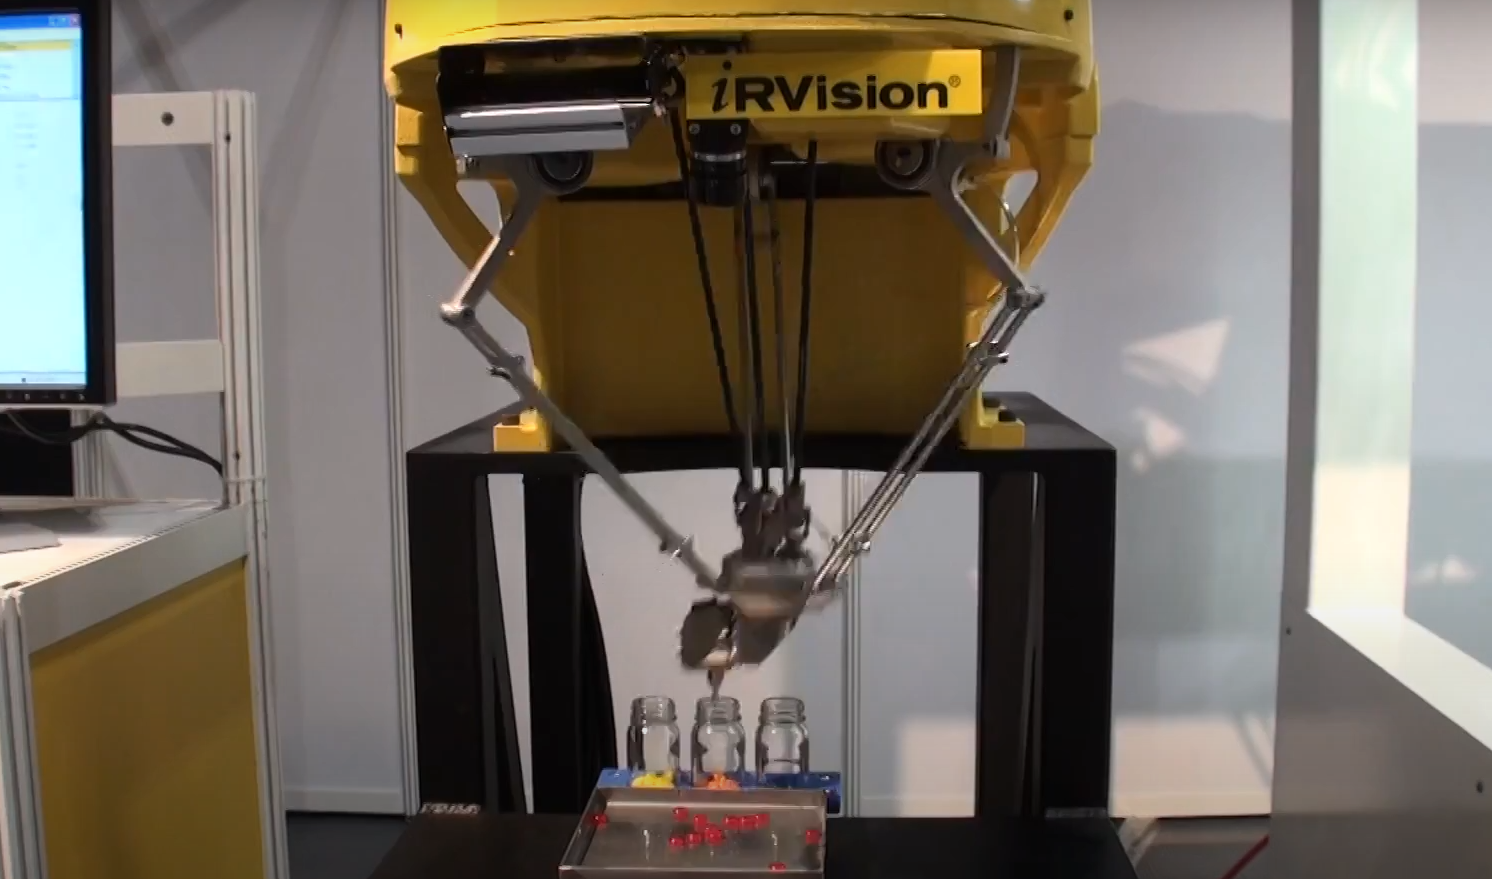
\includegraphics[width=0.8\textwidth]{Images/Chap2/FANUC.png}
        \caption[FANUC M‑1iA – Pill Sorting Demonstration Cell]{FANUC M‑1iA – Pill Sorting Demonstration Cell}
        \label{fig:FANUC_PillSorting}
    \end{figure}
    \item \textbf{ABB IRB 360 – Snack Sorting and Packaging Cell}: An ABB IRB 360 robot with a PickMaster vision system sorts and packages snacks at high speed, demonstrating a food packaging application \cite{ABB}\hyperref[sec:bibliography]{[4]}. The cell is illustrated in Figure \ref{fig:ABB_SnackSorting}.
   \begin{figure}[H]
    \centering
    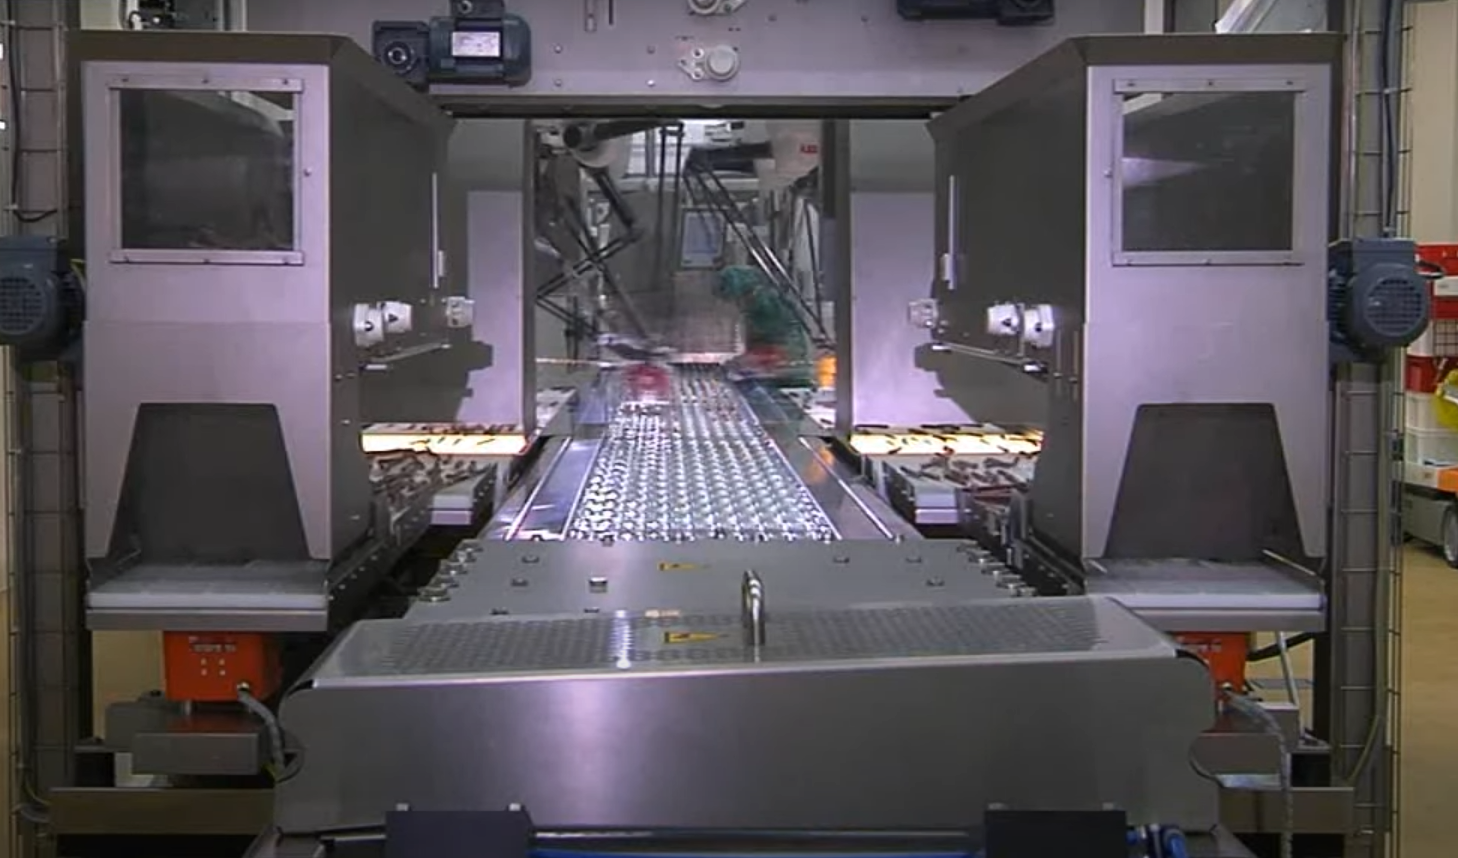
\includegraphics[width=0.45\textwidth]{Images/Chap2/ABB1.png}
    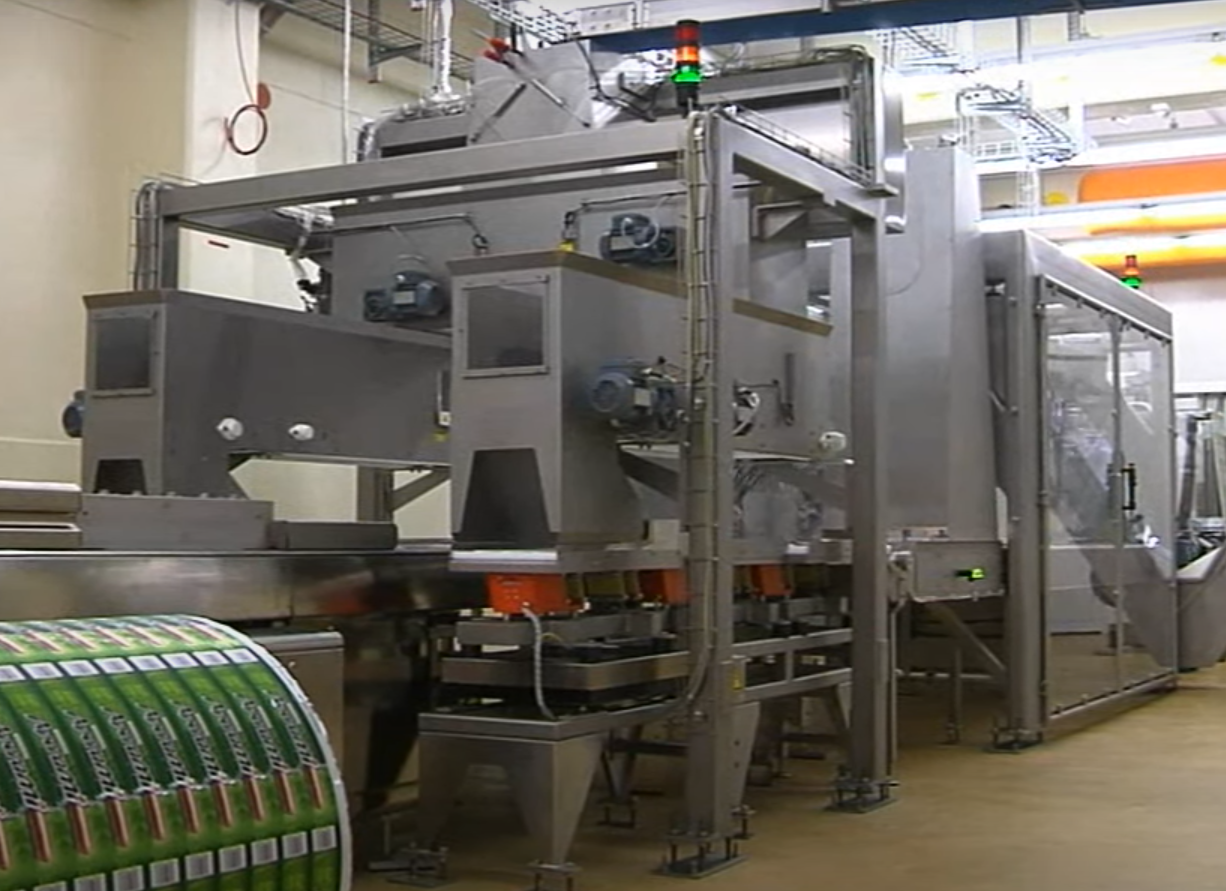
\includegraphics[width=0.45\textwidth]{Images/Chap2/ABB2.png}
    \caption[ABB IRB 360 – Snack Sorting and Packaging Cell]{ABB IRB 360 – Snack Sorting and Packaging Cell}
    \label{fig:ABB_SnackSorting}
\end{figure}
    \item \textbf{ZenRobotics Recycler – Waste Sorting Cell}: This autonomous waste sorting system combines robotic arms, cameras, and AI to separate materials like metal and plastic from construction waste, processing up to 3000 objects per hour \cite{ZenRobotics}\hyperref[sec:bibliography]{[5]}. An example of this system is shown in Figure \ref{fig:ZenRobotics_WasteSorting}.
    \begin{figure}[H]
        \centering
        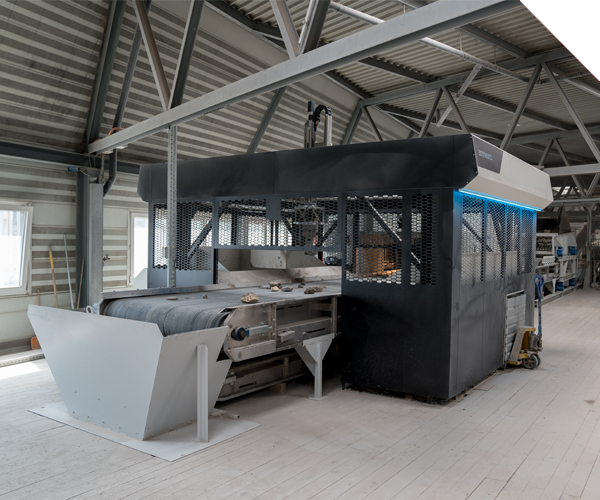
\includegraphics[width=0.6\textwidth]{Images/Chap2/ZenRobotics.png}
        \caption[ZenRobotics Recycler – Waste Sorting Cell]{ZenRobotics Recycler – Waste Sorting Cell}
        \label{fig:ZenRobotics_WasteSorting}
    \end{figure}
\end{itemize}

\section{Hardware Architecture}
The hardware architecture encompasses all physical components, including the operative part (sensors and actuators), the control part (PLC, HMI, robot controller), and supporting systems.

\subsection{Operative Part}
This part consists of the physical elements that interact directly with the environment, including actuators and sensors.

\subsubsection{Actuators}
\begin{itemize}
  \item \textbf{KUKA Robot - KR AGILUS}: The six-axis KUKA KR AGILUS robot was chosen as the main manipulator due to its compact size, high speed, and exceptional repeatability of $\pm0.03$ mm. It is controlled by a KRC4 Compact controller that communicates with the PLC via industrial Ethernet. The robot's technical specifications are detailed in Table \ref{tab:kuka_specs}. A visual representation of the robot is provided in Annex \ref{fig:KukaRobot}, and its six-axis configuration is shown in Annex \ref{fig:KukaAxis}.
    \renewcommand{\arraystretch}{1.3} 
    \begin{table}[H] 
    \centering 
    \caption{Technical Specifications of the KR AGILUS Robot} 
    \label{tab:kuka_specs} 
    \begin{tabularx}{\textwidth}{|l|X|} 
     \hline 
     \textbf{Parameter} & \textbf{Value} \\ 
     \hline 
     Model & KR 6 R700 (AGILUS series) \\ 
     \hline 
     Degrees of Freedom & 6 axes \\ 
     \hline 
     Maximum Payload & 6 kg \\ 
     \hline 
     Reach & 706.7 mm \\ 
     \hline 
     Repeatability & $\pm0.03$ mm \\ 
     \hline 
     Controller & KRC4 Compact \\ 
     \hline 
     Protection Rating & IP54 \\ 
     \hline 
     Mounting Positions & Floor, ceiling, wall \\ 
     \hline 
    \end{tabularx} 
    \end{table}
    

    
    \item \textbf{Belt Conveyors}: Two perpendicular Dierre belt conveyors create a compact L-shaped flow for transporting colored cubes. Each is powered by an SMT 5634 geared motor and controlled by the PLC to operate at a fixed speed. The main specifications are listed in Table \ref{tab:conveyor_specs}. The conveyor belt used in the cell is shown in Figure \ref{fig:conveyor_real}.
    
    \renewcommand{\arraystretch}{1.3}
    \setlength{\tabcolsep}{10pt}
    
    \begin{table}[H]
        \centering
        \caption{Technical Specifications of the Conveyor System}
        \label{tab:conveyor_specs}
        \begin{tabularx}{\textwidth}{|l|X|}
            \hline
            \textbf{Parameter} & \textbf{Value} \\
            \hline
            Manufacturer & Dierre \\
            \hline
            Motor & SMT 5634 \\
            \hline
            Control Method & PLC-controlled contactor \\
            \hline
            Speed & Fixed \\
            \hline
            Dimensions & Approx. 1000 mm length / 150 mm width \\
            \hline
        \end{tabularx}
    \end{table}

    \begin{figure}[H]
        \centering
        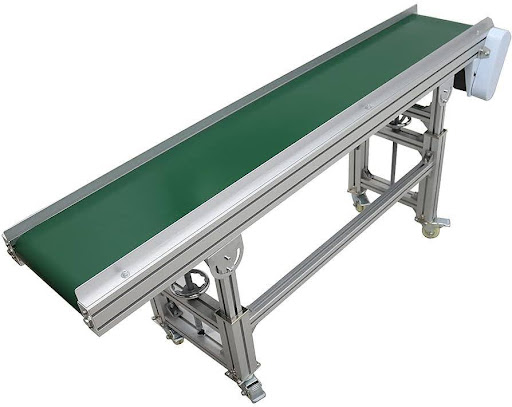
\includegraphics[width=0.35\textwidth]{Images/Chap2/Conveyor.jpg}
        \caption[Conveyor Belt Used in the Sorting Cell]{Dierre conveyor belt used for part transport}
        \label{fig:conveyor_real}
    \end{figure}

    \item \textbf{Pneumatic Cylinders}: Two Festo guided cylinders were integrated for precise, stable linear motion to push cubes into position. Their compact design was ideal for the limited space. An example of the cylinder used is shown in Figure \ref{fig:Festo_Cylinder}.
    \begin{figure}[H]
        \centering
        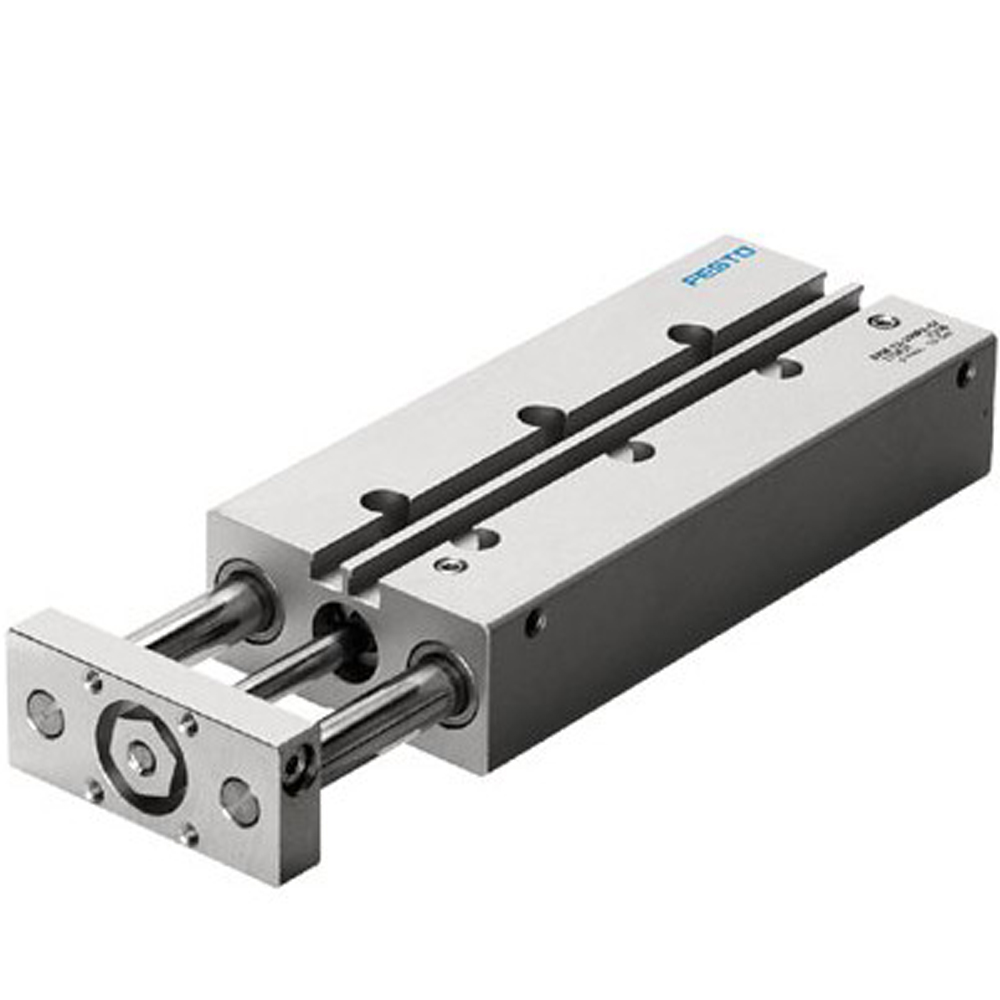
\includegraphics[width=0.32\textwidth]{Images/Chap2/verin.jpg}
        \caption[Festo Guided Pneumatic Cylinder]{Festo Guided Pneumatic Cylinder}
        \label{fig:Festo_Cylinder}
    \end{figure}

    \item \textbf{Prehenseur (Gripper)}: A custom-designed pneumatic parallel jaw gripper, specifically a Festo type, was developed as the robot's end-effector. This device uses a pneumatic cylinder to provide the gripping force and is sized to securely handle the colored cubes. The gripper is shown in Figure \ref{fig:gripper}.
    \begin{figure}[H]
        \centering
        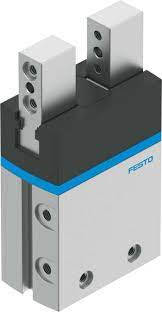
\includegraphics[width=0.18\textwidth]{Images/Chap2/gripper.jpg}
        \caption[Pneumatic Parallel Jaw Gripper]{Pneumatic Parallel Jaw Gripper}
        \label{fig:gripper}
    \end{figure}
\end{itemize}

\subsubsection{Sensors}
In the designed sorting cell, a set of sensors was integrated to enable real-time feedback and ensure accurate synchronization between the different automated components, including conveyors, pneumatic actuators, and the robot. These sensors play a critical role in detecting the presence of objects, confirming part positions, and triggering control events within the PLC logic.

\begin{itemize}
    \item \textbf{OMRON E3Z-D61 2M}:
    Two OMRON E3Z-D61 photoelectric sensors were integrated into the sorting cell to detect the presence of cubes during critical stages of the process. One sensor was placed in front of the guided cylinder, between the two conveyors, and the other in front of the vision system camera. These sensors were chosen for their compact size, diffuse detection capability, and reliable performance with colored plastic objects under varying ambient lighting.
    The main characteristics and functions of the installed sensors are summarized in Table \ref{tab:omron_specs}. A visual representation of the sensor is shown in Figure \ref{fig:Omron_Sensor}.
    \renewcommand{\arraystretch}{1.3}
    \setlength{\tabcolsep}{10pt}
    
    \begin{table}[H]
        \centering
        \caption{OMRON E3Z-D61 Sensor Specifications}
        \label{tab:omron_specs}
        \begin{tabularx}{\textwidth}{|l|X|}
            \hline
            \textbf{Parameter} & \textbf{Value} \\
            \hline
            Sensing method & Diffuse reflective \\
            \hline
            Sensing distance & 100 mm \\
            \hline
            Min sensing distance & 5 mm \\
            \hline
            Response time & 1 ms \\
            \hline
            Width & 10.8 mm \\
            \hline
            Height & 31 mm \\
            \hline
            Depth & 20 mm \\
            \hline
            Type of light & Infrared light \\
            \hline
            Power supply voltage & 12-24 V \\
            \hline
        \end{tabularx}
    \end{table}

    \begin{figure}[H]
        \centering
        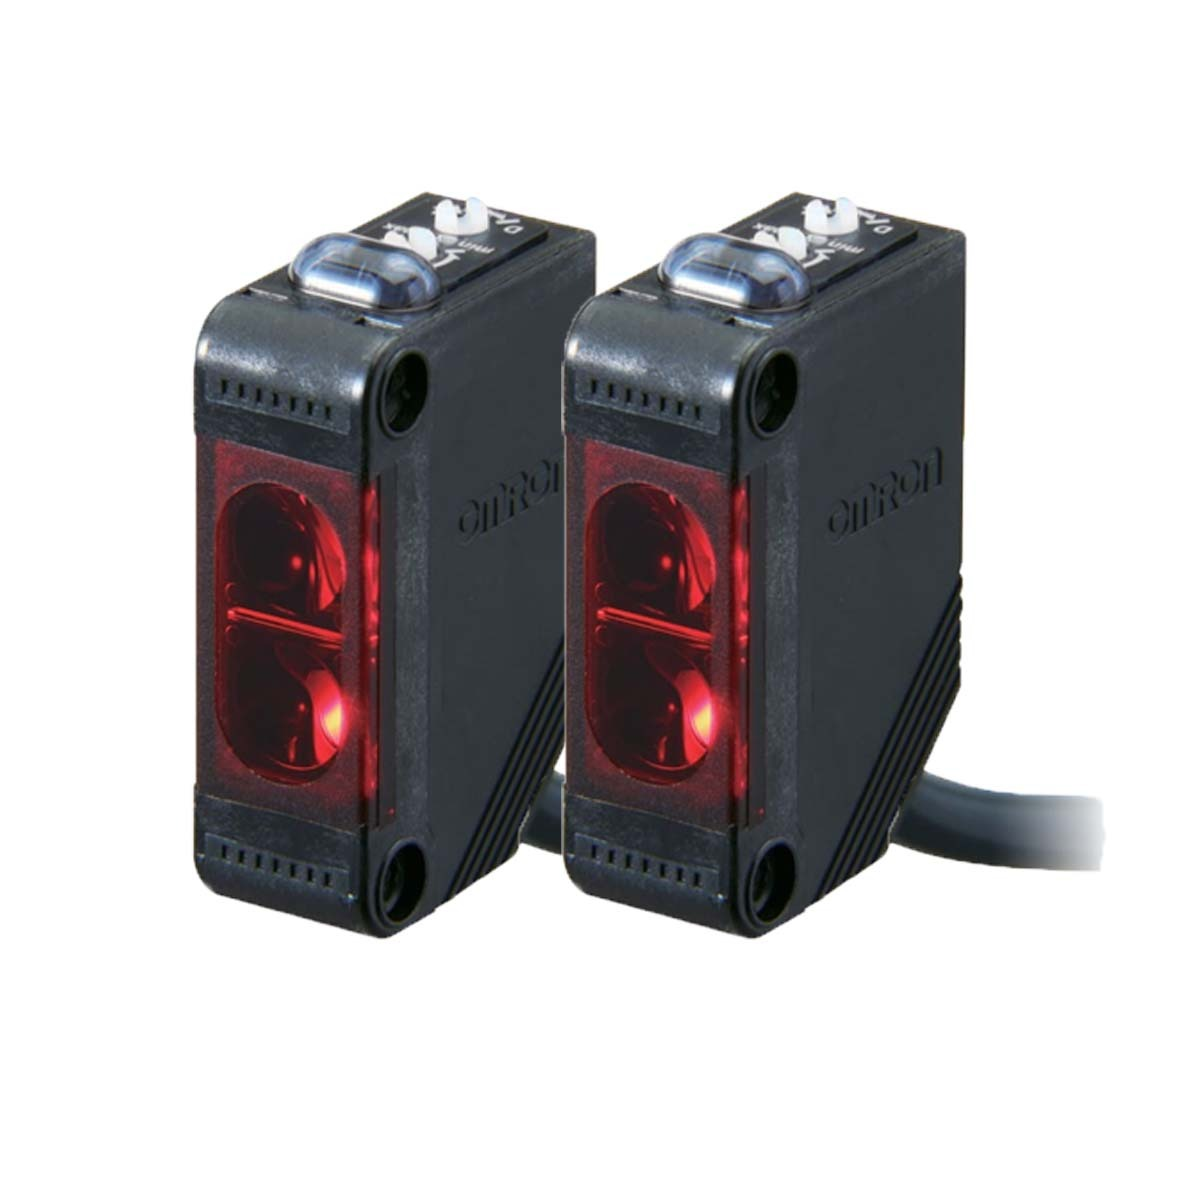
\includegraphics[width=0.4\textwidth]{Images/Chap2/OmronSensor.jpg}
        \caption[OMRON E3Z-D61 Sensor]{OMRON E3Z-D61 Sensor}
        \label{fig:Omron_Sensor}
    \end{figure}

    \item \textbf{Proximity Sensors for Cylinders (FESTO SMT-8M-A-PS-24V-E-0,3-M8D)}
    
    To ensure accurate control and positioning of the pneumatic actuators, Festo SMT-8M-A-PS-24V-E-0,3-M8D proximity sensors were installed on each cylinder. These sensors detect the piston’s position and provide feedback to the PLC, allowing precise monitoring of the extension and retraction states.
    A total of five sensors were used across the system. Two sensors were mounted on each of the two main guided cylinders to detect both end positions. The remaining sensor was placed on the final storage-area cylinder, where only the fully extended position needed to be confirmed. This configuration ensures that the system always has reliable information on whether a part has been moved, aligned, or stored correctly.
    
    These magnetic proximity sensors offer non-contact detection, resulting in long service life, resistance to mechanical wear, and quick response time. Their compact format and easy mounting grooves make them ideal for cylinder-based installations. The sensors were directly wired to the PLC's digital input terminals, enabling real-time logic decisions within the automation sequence.
    
    The technical specifications of the sensors are summarized in Table \ref{tab:festo_proximity_specs}. A visual representation of the sensor is provided in Figure \ref{fig:Festo_Proximity_Sensor}.
    \renewcommand{\arraystretch}{1.3}
    \setlength{\tabcolsep}{10pt}
    \begin{table}[H]
        \centering
        \caption{Technical Specifications of the Festo Cylinder Proximity Sensors}
        \label{tab:festo_proximity_specs}
        \begin{tabularx}{\textwidth}{|l|X|}
            \hline
            \textbf{Parameter} & \textbf{Value} \\
            \hline
            Manufacturer & Festo \\
            \hline
            Type & Magnetic proximity sensor for pneumatic cylinders \\
            \hline
            Quantity & 5 (2 per cylinder on main axes, 1 for storage cylinder) \\
            \hline
            Detection Type & Magnetic field detection (non-contact) \\
            \hline
            Application & Detect end-of-stroke positions of pneumatic actuators \\
            \hline
            Mounting & Integrated groove on cylinder body \\
            \hline
            Connection Type & Cable with connector to PLC input \\
            \hline
            Response Time & Switch-on time : < 1.3 ms / Switch-off time : < 7.3 ms \\
            \hline
            Advantages & Long service life, wear-free, compact, easy installation \\
            \hline
            Operational voltage range DC & 5 V ... 30 V \\
            \hline
        \end{tabularx}
    \end{table}
    \begin{figure}[H]
        \centering
        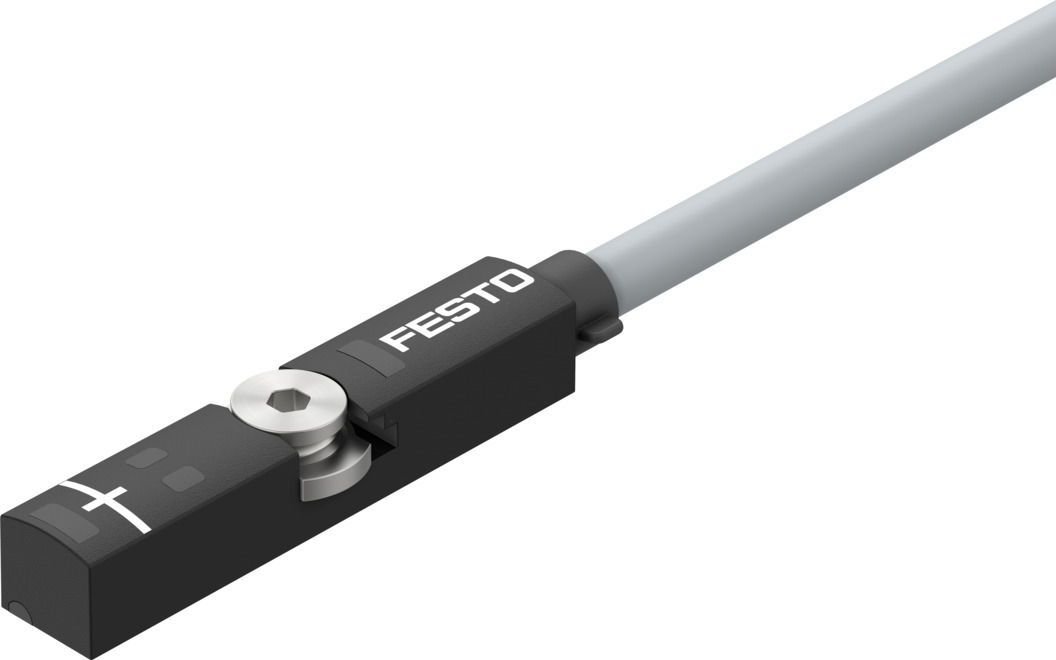
\includegraphics[width=0.35\textwidth]{Images/Chap2/proximetsensor.jpg}
        \caption[ Festo Proximity Sensors for Cylinders ]{Festo Proximity Sensors for Cylinders}
        \label{fig:Festo_Proximity_Sensor}
    \end{figure}
\end{itemize}





\subsection{Control Part}
The control part includes all the components responsible for managing and coordinating the actions of the automated system. It interprets sensor data, executes logical decisions, and generates appropriate commands to drive actuators. This part typically consists of programmable logic controllers (PLCs), human-machine interfaces (HMIs), and communication modules. Together, these elements ensure that the system operates safely, efficiently, and in accordance with predefined sequences.

\begin{itemize}
    \item \textbf{Programmable Logic Controller (PLC)}:

    The programmable logic controller (PLC) is the core of the control system. It processes sensor inputs, executes the automation logic, and drives the actuators accordingly. In this project, the PLC is responsible for managing the entire sorting cycle, including cylinder control, conveyor coordination, sensor supervision, and real-time interaction with the HMI and external devices such as the industrial robot and Raspberry Pi. A digital-only I/O configuration was required, and network-based communication played a key role in the component selection process.


    The selection of the programmable logic controller (PLC) was based on key functional requirements derived from the automation and communication needs of the sorting cell. These requirements included:
    
    -At least 11 digital inputs (e.g., sensors, endstops, Buttons)
    
    -At least 11 digital outputs (e.g., solenoid valves, conveyor motors, Lights)
    
    -Three Ethernet connections (Robot controller, Raspberry Pi, HMI)

    The selected PLC had to support Siemens' TIA Portal ecosystem and provide expansion flexibility while keeping the total cost within a reasonable budget. Two possible configurations from different Siemens product families were considered and compared based on their I/O capacity, communication features, and overall cost, as shown in Table \ref{tab:plc_siemens_comparison}.
    \renewcommand{\arraystretch}{1.3}
    \setlength{\tabcolsep}{8pt}

    \begin{table}[H]
        \centering
        \caption{Comparison of Siemens PLC Configurations}
        \label{tab:plc_siemens_comparison}
        \begin{tabularx}{\textwidth}{|l|X|X|X|X|}
            \hline
            \textbf{Solution} & \textbf{PLC Family and Modules} & \textbf{I/O Capacity} & \textbf{Ethernet Support} & \textbf{Estimated Cost (€)} \\
            \hline
            \textbf{A} & \textbf{S7-1212C} + SB module + Ethernet switch & 14 DI / 10 DO + 4 DI / 2 DO & 1 (add switch to split) & ~350 € \\
            \hline
            \textbf{C} & \textbf{S7-1500 (CPU 1511)} + SM1223 module & 14 DI / 10 DO + 8 DI / DO & 2 native ports + Profinet & ~650 € \\
            \hline
        \end{tabularx}
    \end{table}

    After evaluating the available options, Solution A, based on the S7-1212C from the S7-1200 series, was selected. This choice provided a good balance between I/O capacity, communication flexibility, and cost. The Siemens S7-1212C is shown in Figure \ref{fig:siemens_plc}.

    Although the base CPU only includes one Ethernet port, a standard industrial Ethernet switch was added to fulfill the requirement for three simultaneous Ethernet connections. The input/output capacity was covered using a compact signal board (SB), and the option for additional expansion modules remains available if future needs arise.

    This solution ensured full integration with the Siemens TIA Portal environment, supported Profinet communication with the robot and HMI, and kept the system modular and maintainable for demonstration and industrial fair use.

    \begin{figure}[H]
        \centering
        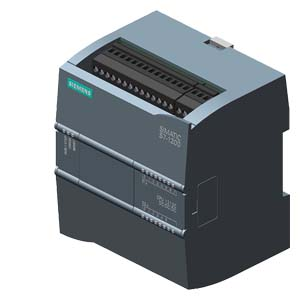
\includegraphics[width=0.3\textwidth]{Images/Chap2/PLC.jpg}
        \caption[Siemens S7-1212C ]{Siemens S7-1212C}
        \label{fig:siemens_plc}
    \end{figure}
    
    \item \textbf{Human-Machine Interface (HMI)}:

    The Human-Machine Interface (HMI) enables system supervision and interaction, providing real-time feedback to the operator regarding the sorting cycle, sensor states, and manual overrides. The selected HMI had to support Siemens' WinCC Unified platform to enable both local touchscreen operation and remote control through a standard web browser, which is particularly useful for demonstration and maintenance purposes during trade fairs. A visual representation of the panel is shown in Figure \ref{fig:tp1200}.

    To satisfy the visualization and usability requirements, a \textbf{12-inch Siemens Unified Comfort Panel} was selected. Specifically, the \textbf{TP1200 Unified} panel was chosen as it offers a high-resolution display, Unified Runtime support, and Profinet communication capabilities at a reasonable cost. Its compatibility with TIA Portal and Unified architecture ensures seamless integration with the control system.

    Additional implementation details regarding screen content and remote access will be addressed in later sections.

    \begin{figure}[H]
        \centering
        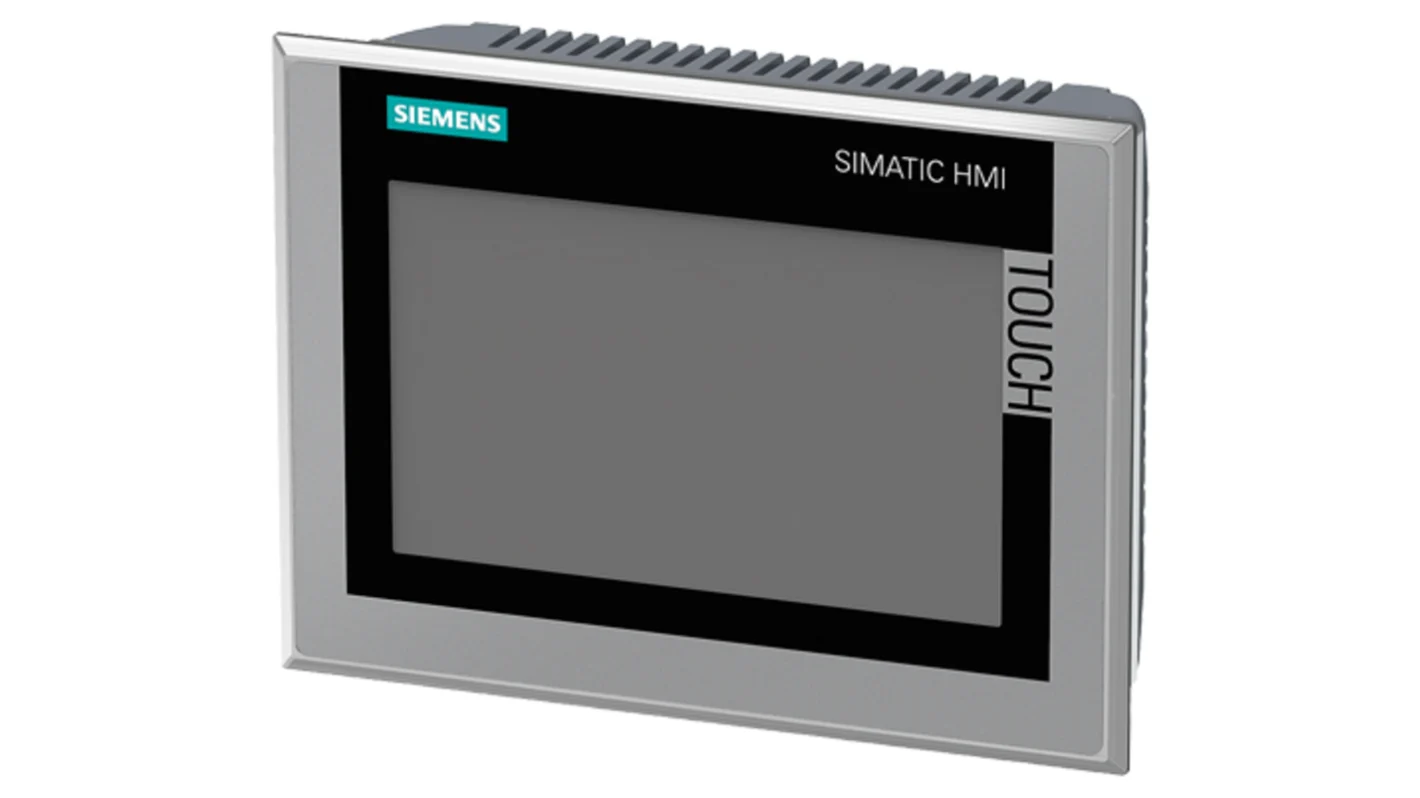
\includegraphics[width=0.5\textwidth]{Images/Chap2/TP1200_Unified.png} % replace with actual path
        \caption[TP1200 Unified Comfort Panel]{TP1200 Unified Comfort Panel (12.1") }
        \label{fig:tp1200}
    \end{figure}
    
    \item \textbf{Robot Controller}:

    The KUKA industrial robot used in this project is managed through a \textbf{KRC4 Compact} controller, which serves as the interface between the robot and the rest of the automation system. This controller handles the motion logic, safety configurations, and communication protocols necessary to integrate the robot into the control architecture. The KRC4 Compact Controller is shown in Figure \ref{fig:krc4compact}.

    The controller is configured using KUKA.WorkVisual software, which allows the setup of I/O mappings and Profinet communication. In this setup, the KRC4 Compact operates as a Profinet device connected to the PLC, allowing synchronization with the overall automation sequence.

    \begin{figure}[H]
        \centering
        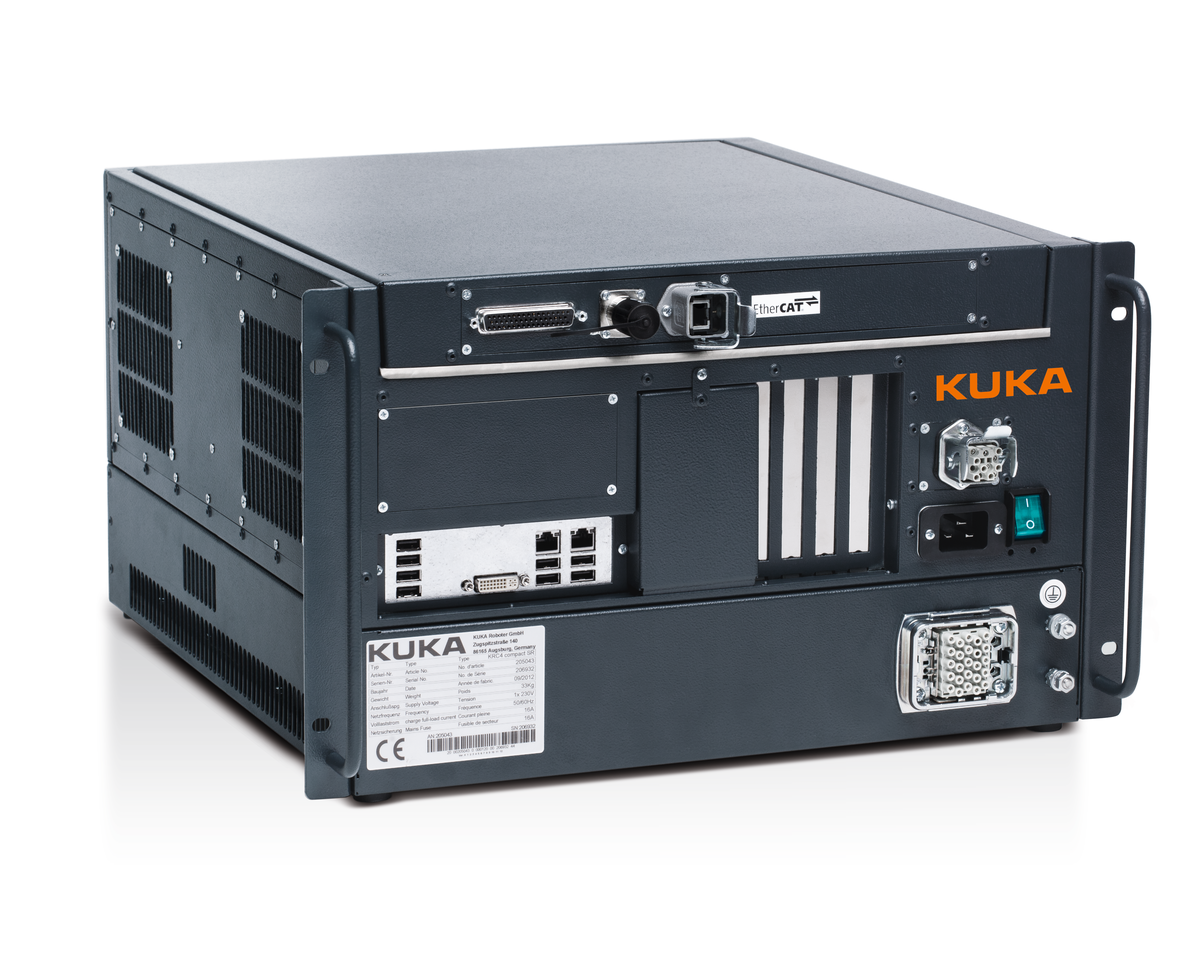
\includegraphics[width=0.45\textwidth]{Images/Chap2/KRC4.png} % replace with actual image
        \caption[KRC4 Compact Controller]{KUKA KRC4 Compact Robot Controller}
        \label{fig:krc4compact}
    \end{figure}

\end{itemize}

\subsection{Electrical Cabinet}
The electrical cabinet serves as the central hub for power distribution, protection, and control within the automated system. All main control components—including the PLC, contactors, power supplies, terminals, and circuit protection devices—are housed inside this enclosure. The cabinet ensures safe and organized wiring, while also facilitating maintenance and future scalability.

\subsubsection{Electrical Wiring Diagram}
To ensure the correct integration and protection of all electrical components, a detailed wiring diagram was created. This diagram represents the overall electrical architecture, including power distribution, component connections, protection devices, and control wiring, and can be seen in Annex \ref{fig:electrical_diagram}.


\subsubsection{Protection components}
This section details the essential components used for circuit protection within the electrical cabinet. These components are vital for safeguarding the entire system against electrical faults, such as overcurrents and short-circuits. By ensuring the integrity of the circuits, they prevent damage to expensive equipment and, more importantly, guarantee the safety of the operating environment. The specific components are outlined in \ref{tab:protection_components}.

\begin{table}[H]
    \centering
    \caption{Protection Components Used in the Electrical Cabinet}
    \label{tab:protection_components}
    \begin{tabularx}{\textwidth}{| >{\raggedright}p{0.3\textwidth} | >{\centering}m{0.2\textwidth} | >{\centering\arraybackslash}m{2.3cm} | X |}
        \hline
        \textbf{Name and Description} & \textbf{Brand} & \textbf{Figure} & \textbf{Function} \\
        \hline
        \textbf{Motor circuit breaker, TeSys GV2, 3P, 4-6.3 A, thermal magnetic, screw clamp terminals} & Schneider Electric &
        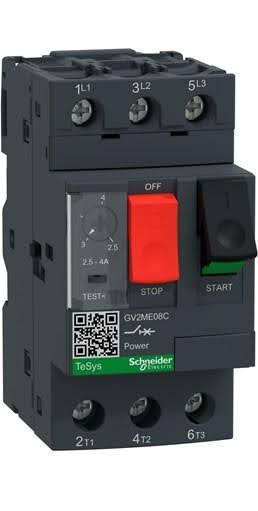
\includegraphics[width=2cm]{Images/Chap2/TeSys GV2.jpg} & Provides overload and short-circuit protection for motor circuits. \\
        \hline
        \textbf{Overcurrent circuit breaker Easy9, 1P+N, 16A, curve C, 4.5kA, type CA, 30mA} & Schneider Electric &
        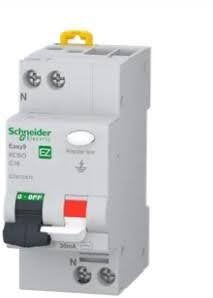
\includegraphics[width=2.2cm]{Images/Chap2/Schneider1.jpg} & Provides overcurrent and differential protection. \\
        \hline
    \end{tabularx}
\end{table}
\subsubsection{Power converters components}
This section outlines the power converter components responsible for providing stable DC power to the system's control elements. These components are listed in Table \ref{tab:power_converter_components}.
\begin{table}[H]
    \centering
    \caption{Power Converter Components Used in the Electrical Cabinet}
    \label{tab:power_converter_components}
    \begin{tabularx}{\textwidth}{| >{\raggedright}p{0.3\textwidth} | >{\centering}m{0.2\textwidth} | >{\centering\arraybackslash}m{2.5cm} | X |}
        \hline
        \textbf{Name and Description} & \textbf{Brand} & \textbf{Figure} & \textbf{Function} \\
        \hline
        \textbf{Power Supply MDR-60-24} & Mean Well &
        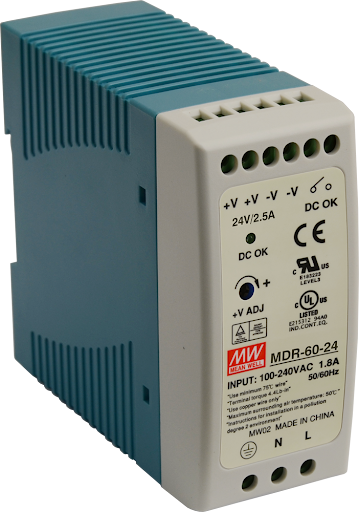
\includegraphics[width=2.2cm]{Images/Chap2/MeanWell.png} & Provides stable 24V DC power to the PLC, sensors, contactors, and other control components. \\
        \hline
        \textbf{Power Supply MDR-60-5} & Mean Well &
        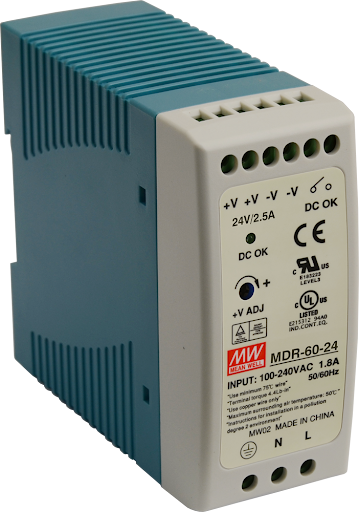
\includegraphics[width=2.2cm]{Images/Chap2/MeanWell.png} & Provides stable 5V DC power to Power the Raspberry Pi. \\
        \hline
    \end{tabularx}
\end{table}

\subsubsection{Control components}
This section details the primary control and logic components of the electrical system. The components used are listed in Table \ref{tab:control_components}.
\begin{table}[H]
    \centering
    \caption{Control Components Used in the Electrical Cabinet}
    \label{tab:control_components}
    \begin{tabularx}{\textwidth}{| >{\raggedright}p{0.3\textwidth} | >{\centering}m{0.2\textwidth} | >{\centering\arraybackslash}m{2.8cm} | X |}
        \hline
        \textbf{Name and Description} & \textbf{Brand} & \textbf{Figure} & \textbf{Function} \\
        \hline
        \textbf{S7-1200 PLC (CPU 1214C)} & Siemens &
        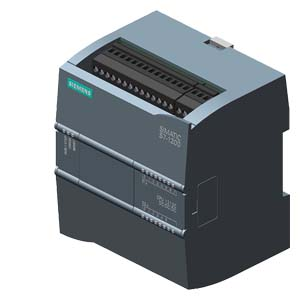
\includegraphics[width=2.5cm]{Images/Chap2/PLC.jpg} & Controls the system logic, managing inputs/outputs, safety signals, and emergency stops. \\
        \hline
        \textbf{ Contactor 
        -TeSys LC1-D - 3 poles - AC-3 440V 18 A - coil 24 V AC} & Schneider Electric &
        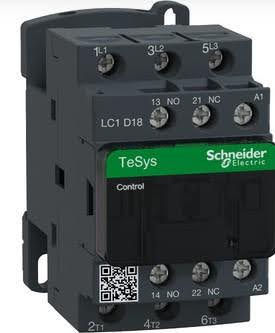
\includegraphics[width=2.5cm]{Images/Chap2/TeSys LC1.jpg} & Used to switch AC loads like conveyor motors. It acts as a safety device, cutting power when the emergency button is pressed. \\
        \hline
        \textbf{Key Selector Switch - Harmony XB4 - 3131A key switch - Ø22 - 2 pos fixed - spring return G } & Schneider Electric &
        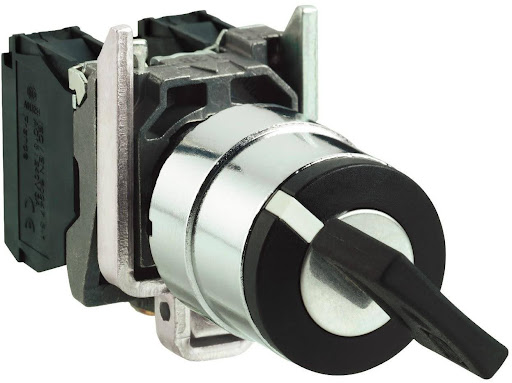
\includegraphics[width=2.5cm]{Images/Chap2/Harmony XB4.jpg} & Allows the operator to switch the main power on or off. \\
        \hline
        \textbf{LED Indicator Light - Harmony XB4 - LED indicator - Ø22 - red - 230V} & Schneider Electric &
        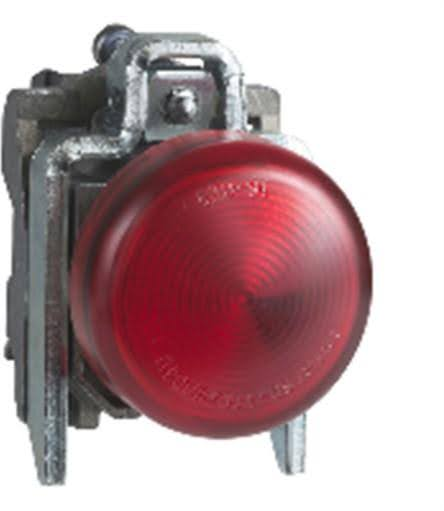
\includegraphics[width=2.5cm]{Images/Chap2/voyant lumineux DEL.jpg} & Indicates system power status. \\
        \hline
        \textbf{Green Push Button - Harmony XB4 - impulse push button - Ø22 - green - 1F} & Schneider Electric &
        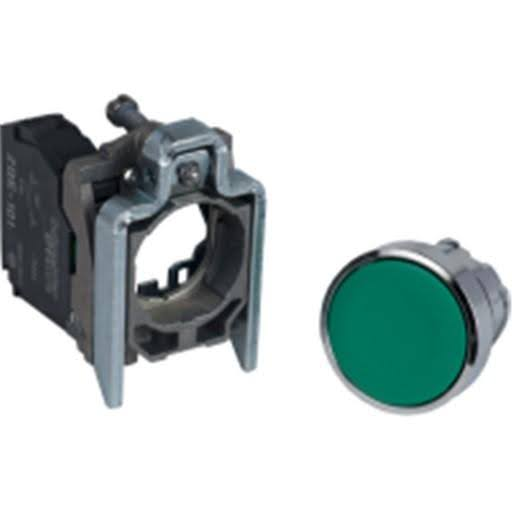
\includegraphics[width=2.5cm]{Images/Chap2/bouton poussoir à impulsion.jpg} & Used to start the system. \\
        \hline
        \textbf{Black Push Button - Harmony XB4 - impulse push button - Ø22 - black - 1F} & Schneider Electric &
        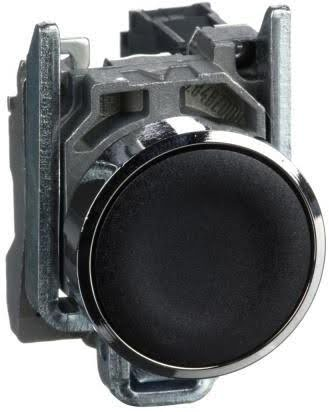
\includegraphics[width=2.5cm]{Images/Chap2/Harmony XB4 - bouton poussoir à impulsio.jpg} & Used to stop or reset the system. \\
        \hline
        \textbf{Emergency Stop Push Button - XB4 emergency stop push button - Harmony- Ø 22mm - red - push/pull} & Schneider Electric &
        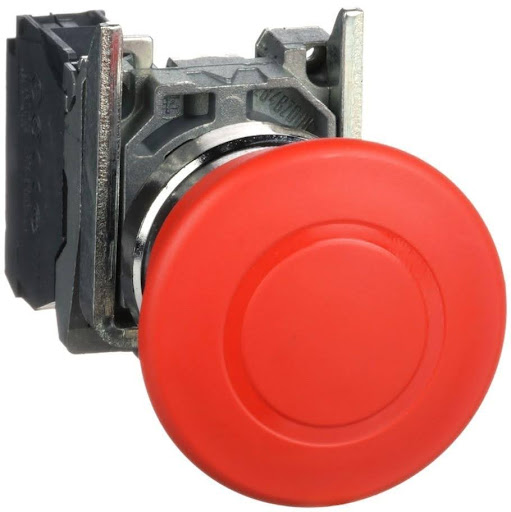
\includegraphics[width=2.5cm]{Images/Chap2/Harmony - bouton poussoir arrêt d'urgence XB4.jpg} & Used for emergency stops to immediately halt all system operations for safety. \\
        \hline
    \end{tabularx}
\end{table}





\subsubsection{Other components}
This section lists additional components and hardware essential for the electrical cabinet's structure and wiring. Table \ref{tab:other_components} provides a list of these components.
\begin{table}[H]
    \centering
    \caption{Other Components Used in the Electrical Cabinet}
    \label{tab:other_components}
    \begin{tabularx}{\textwidth}{| >{\raggedright}p{0.3\textwidth} | >{\centering}m{0.2\textwidth} | >{\centering\arraybackslash}m{2.5cm} | X |}
        \hline
        \textbf{Name and Description} & \textbf{Brand} & \textbf{Figure} & \textbf{Function} \\
        \hline
        \textbf{GT 80-40-25} & Schneider Electric &
        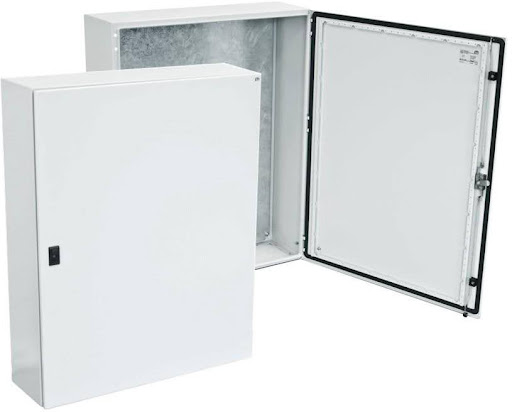
\includegraphics[width=2.5cm]{Images/Chap2/GT 80-40-25.jpg} & Protects electrical and electronic components from dust, moisture, and external impacts. \\
        \hline
        \textbf{Rittal Slotted Panel Trunking, W30 mm x} & Rittal &
        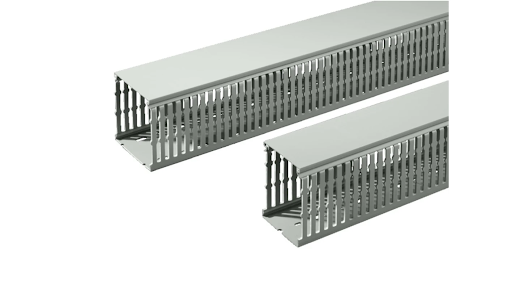
\includegraphics[width=2.5cm]{Images/Chap2/Rittal Slotted Panel Trunki.png} & Organizes and protects cables inside control panels. \\
        \hline
        \textbf{TERMINAL BLOCK WT 16 MM² WKN 16/U V0 GRIS} & Phoenix Contact &
        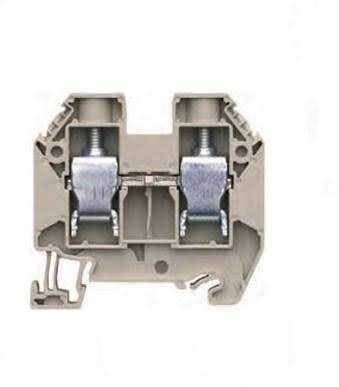
\includegraphics[width=2.5cm]{Images/Chap2/BORNIER.jpg} & Connects and distributes electrical wires safely. \\
        \hline
        \textbf{SZ Support rail to EN 60 715, version TH 35/15, L : 2000 mm} & Phoenix Contact &
        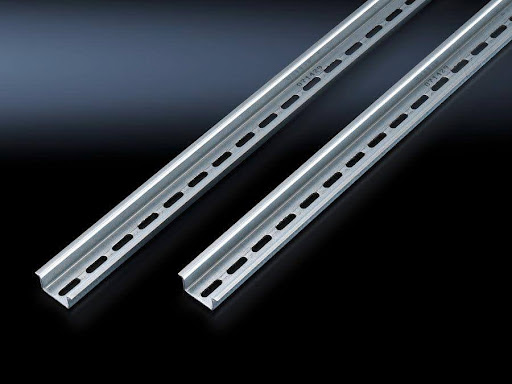
\includegraphics[width=2.5cm]{Images/Chap2/SZ Support rail.jpg} & For snap-mounting terminals or other components with a snap-in system to EN 60 715. \\
        \hline
        \textbf{DS-3E0505-O} & Hikvision &
        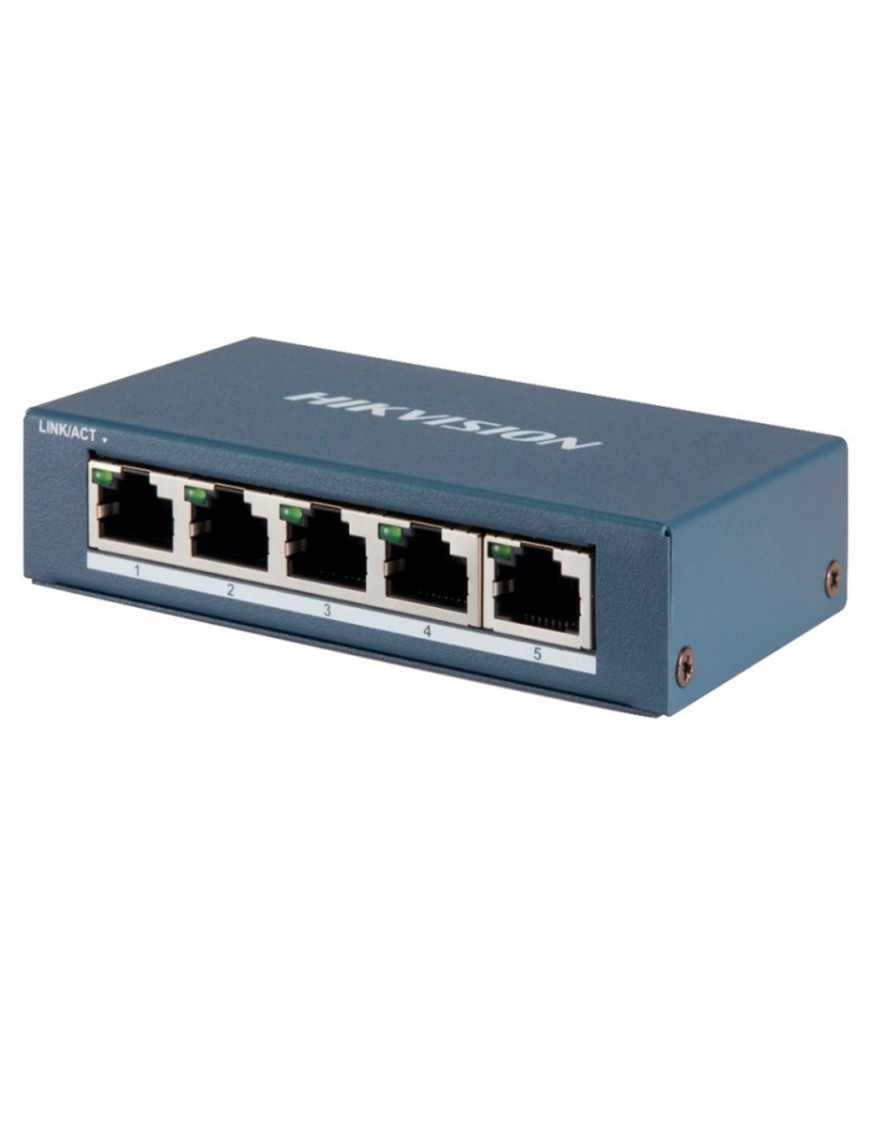
\includegraphics[width=2.5cm]{Images/Chap2/Switch-hikvision-5x-ports-gigabit-unmanaged-tunisie.jpg} & Provides 5 Gigabit RJ45 ports with 1000M network access. \\
        \hline
    \end{tabularx}
\end{table}




\subsubsection{2D and 3D Cabinet Layout}
The following diagrams, generated using E-Plan software, provide a detailed visual representation of the electrical cabinet's layout, as shown in Figure \ref{fig:eplan_layouts}. They illustrate the precise placement of components and the overall physical architecture, ensuring an organized and optimized setup for efficient operation and maintenance.

\begin{figure}[H]
    \centering
    \subfloat[Front door layout]{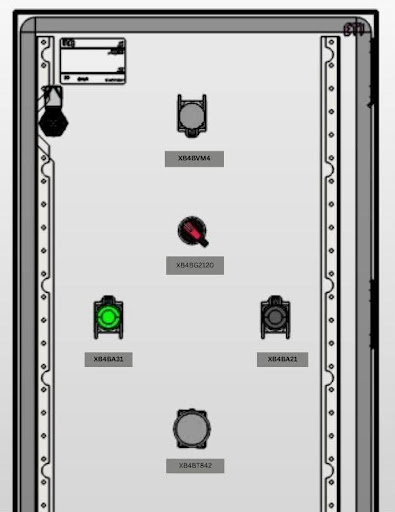
\includegraphics[width=0.3\textwidth]{Images/Chap2/front.jpg}\label{fig:front_door_layout}}
    \hfill % Adds spacing between the images
    \subfloat[Internal layout]{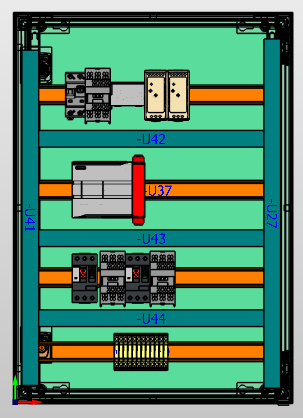
\includegraphics[width=0.28\textwidth]{Images/Chap2/inside.png}\label{fig:internal_layout}}
    \hfill % Adds spacing between the images
    \subfloat[3D View]{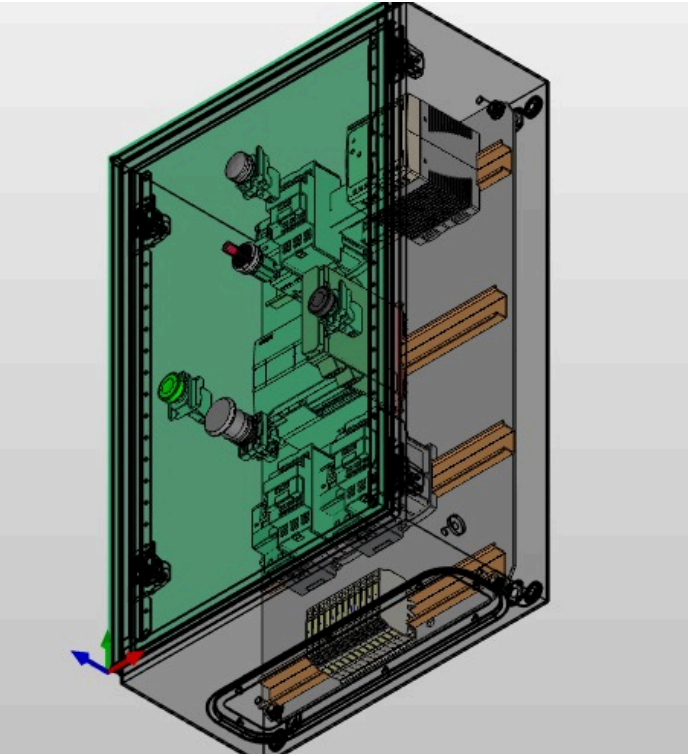
\includegraphics[width=0.3\textwidth]{Images/Chap2/3dlook.png}\label{fig:3d_layout}}
    \caption[E-Plan Electrical Cabinet Layouts]{E-Plan Electrical Cabinet Layouts}
    \label{fig:eplan_layouts}
\end{figure}

\subsection{Pneumatic Cabinet}
The pneumatic cabinet serves as the central hub for compressed air management and motion control within the automated system. It houses all main control components—including air preparation units, distribution manifolds, and solenoid valves—that are essential for the safe and precise operation of pneumatic actuators like cylinders and grippers. The cabinet ensures a clean and organized system, while also facilitating maintenance and future scalability for pneumatic circuits.

\subsubsection{Pneumatic Wiring Diagram}
To ensure the precise operation and sequencing of pneumatic actuators, a detailed wiring diagram was developed. This diagram, along with the components, which are exclusively sourced from Festo, illustrates the controlled flow of compressed air. The pneumatic circuit is presented in Annex \ref{fig:pneumatic_diagram}, which is accompanied by a detailed list of each numbered element, as shown in Table \ref{tab:pneumatic_components}, from the air preparation unit to the final actuators.



\begin{longtable}{|c|p{0.7\textwidth}|}
\caption{Pneumatic Components in the Wiring Diagram}
\label{tab:pneumatic_components}\\
\hline
\textbf{Designation} & \textbf{Description} \\
\hline
\endhead
1 & Parallel Cylinder for Gripper \\
\hline
2 & Guiding Cylinder \\
\hline
3 & Ejector Cylinder \\
\hline
4 & check Valve \\
\hline
5 & 5/3 Directional Valve \\
\hline
6 & 3/2 Directional Valve ( Closed Center ) \\
\hline
7 & Pressure Gauge \\
\hline
8 & Pressure Regulator \\
\hline
9 & flow control valve \\
\hline
10 & Air Treatment Unit \\
\hline
\end{longtable}


\subsubsection{Air Preparation Components}
This subsection details the components responsible for preparing and conditioning the compressed air supply before it is used by the system. The \textbf{FRL (Filter + Regulator + Lubricator) Unit} is a key component for this process, as it prepares the air supply by filtering out impurities, regulating the pressure to a constant level, and adding a small amount of lubricant to the air to ensure smooth operation of the pneumatic components. A visual representation of the FRL unit is provided in Figure \ref{fig:air_prep_components}.

\begin{figure}[H]
\centering
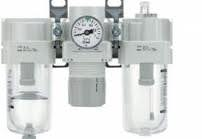
\includegraphics[width=0.4\textwidth]{Images/Chap2/FRLUnit.jpg}
\caption{FRL Unit (Filter + Regulator + Lubricator)}
\label{fig:air_prep_components}
\end{figure}










\subsubsection{Directional Control Valves}
These components are used to direct the flow of compressed air to the actuators, controlling their movement and position. The specific valves used in our system are detailed in Table \ref{tab:directional_valves}.

\begin{longtable}{|p{0.35\textwidth}|c|p{0.5\textwidth}|}
\caption{Directional Control Valves}
\label{tab:directional_valves}\\
\hline
\textbf{Name and Description} & \textbf{Figure} & \textbf{Function} \\
\hline
\endhead
\textbf{5/3 Directional Valve} &
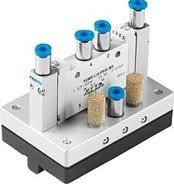
\includegraphics[width=2.5cm]{Images/Chap2/5-3Valve.jpg} & Directs air to cylinders. \\
\hline
\textbf{3/2 Directional Valve} &
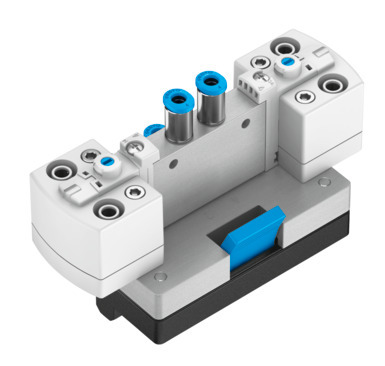
\includegraphics[width=2.5cm]{Images/Chap2/3-2Valve.jpg} & Directs air to cylinders. \\
\hline
\end{longtable}

\subsubsection{Flow and Pressure Control Components}
This section lists components that regulate the pressure and control the speed of air flow to ensure precise movement of the pneumatic actuators. The key components we integrated are shown in Table \ref{tab:flow_pressure_components}.

\begin{longtable}{|p{0.35\textwidth}|c|p{0.5\textwidth}|}
\caption{Flow and Pressure Control Components}
\label{tab:flow_pressure_components}\\
\hline
\textbf{Name and Description} & \textbf{Figure} & \textbf{Function} \\
\hline
\endhead
\textbf{Flow Regulator} &
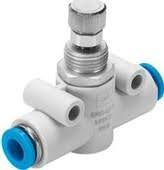
\includegraphics[width=2.5cm]{Images/Chap2/FlowRegulator.jpg} & Controls the air flow rate. \\
\hline
\textbf{Check Valve} &
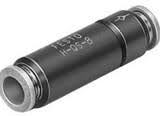
\includegraphics[width=2.5cm]{Images/Chap2/CheckValve.jpg} & Allows one-way airflow only. \\
\hline
\end{longtable}

\subsubsection{Distribution and Safety Components}
This section outlines the essential components for distributing air and ensuring the safety of the pneumatic system. A detailed list of these components is provided in Table \ref{tab:distribution_components}.

\begin{longtable}{|p{0.35\textwidth}|c|p{0.5\textwidth}|}
\caption{Distribution and Safety Components}
\label{tab:distribution_components}\\
\hline
\textbf{Name and Description} & \textbf{Figure} & \textbf{Function} \\
\hline
\endhead
\textbf{Pneumatic Manifold} &
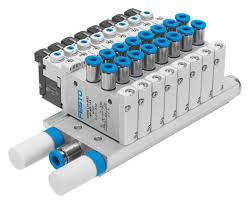
\includegraphics[width=2.5cm]{Images/Chap2/PneumaticManifold.jpg} & Provides a central point for air distribution and serves as a mounting block for multiple control valves, simplifying the circuit. \\
\hline
\textbf{Lockout Valve} &
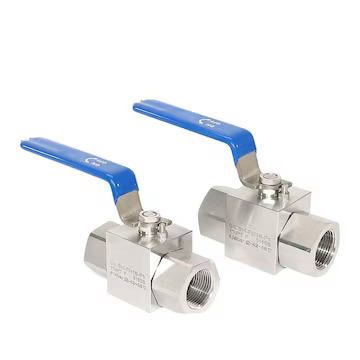
\includegraphics[width=2.5cm]{Images/Chap2/LockoutValve.jpg} & A manual shut-off valve that isolates the pneumatic system from the main air supply for safe maintenance and service. \\
\hline
\textbf{Pneumatic Tubing (4mm)} &
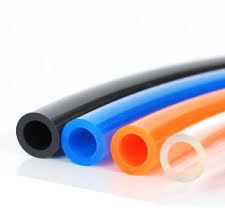
\includegraphics[width=2.5cm]{Images/Chap2/PneumaticTubing.jpg} & Flexible tubing used to create the physical connections for distributing compressed air between all components in the pneumatic circuit. \\
\hline
\end{longtable}







\subsection{Vision System}
The vision system provides the necessary intelligence for color-based classification. Its hardware is designed for reliability and cost-effectiveness in an industrial environment, with the components detailed in Table \ref{tab:vision_hardware}.

\begin{table}[H]
    \centering
    \caption{Vision System Hardware Components}
    \label{tab:vision_hardware}
    \begin{tabularx}{\textwidth}{| >{\raggedright}p{0.4\textwidth} | >{\centering\arraybackslash}m{3.5cm} | X |}
        \hline
        \textbf{Name and Description} & \textbf{Figure} & \textbf{Function} \\
        \hline
        \textbf{Raspberry Pi 4 Model B} &
        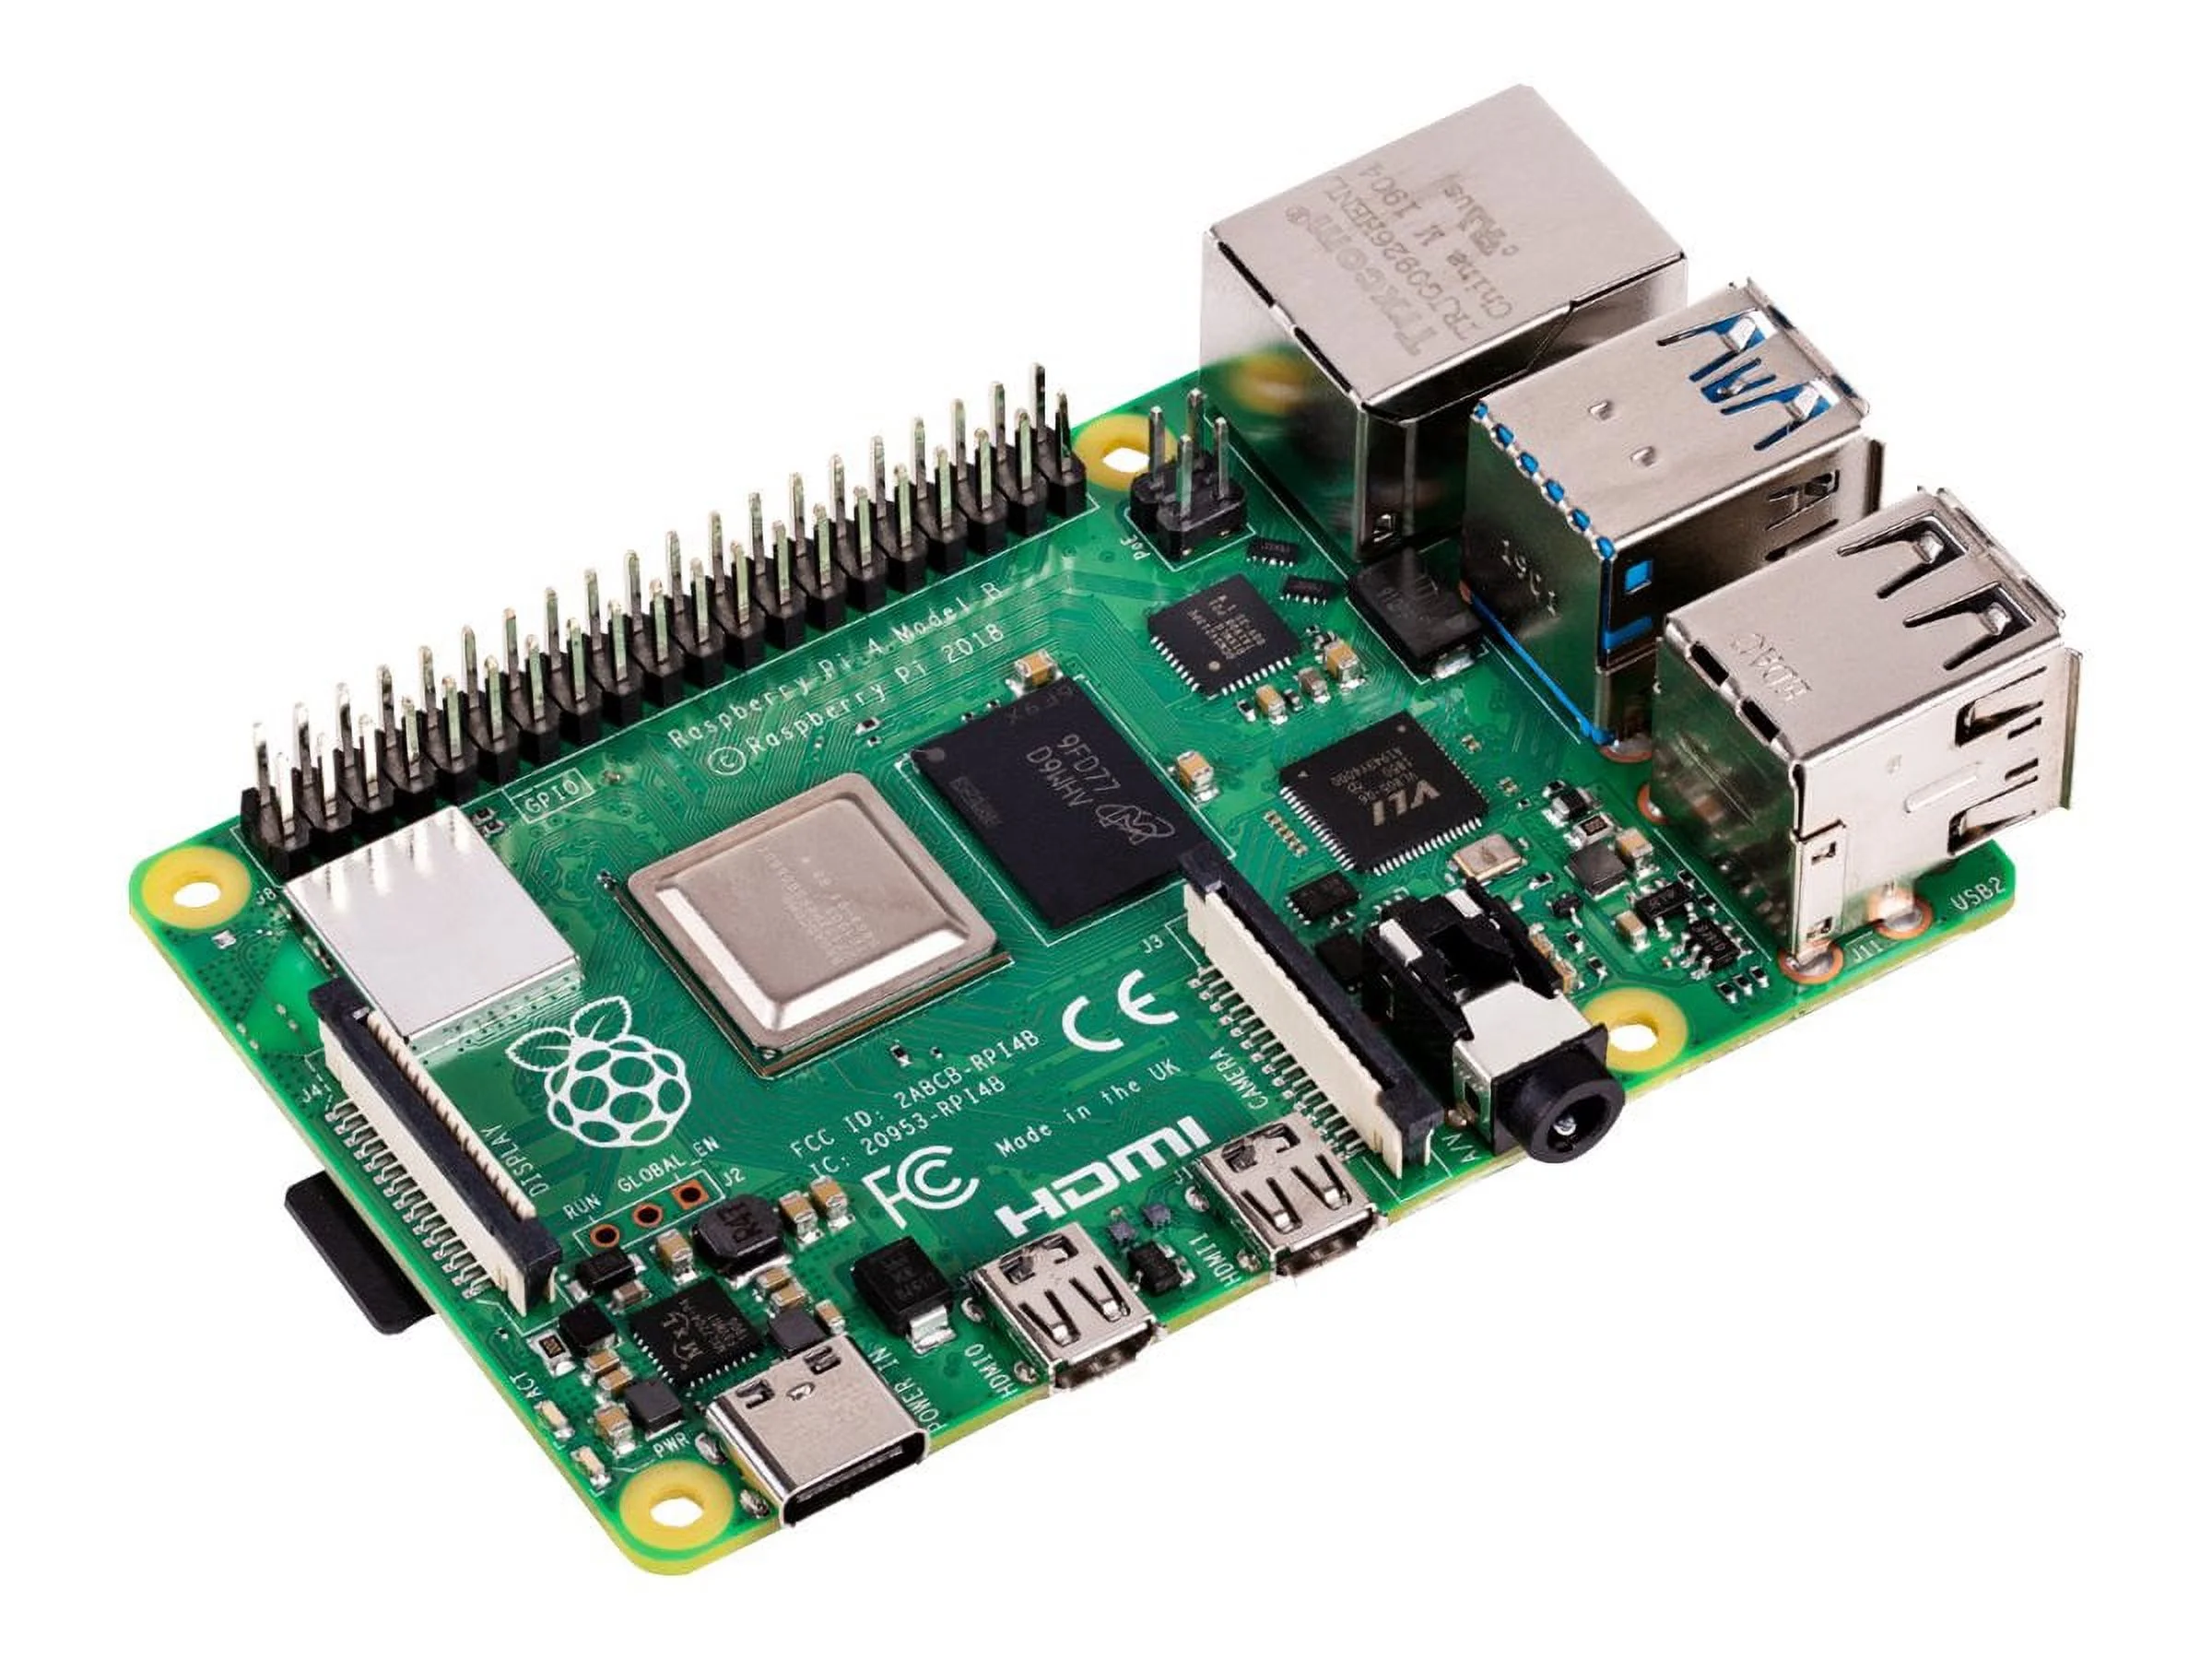
\includegraphics[width=3cm]{Images/Chap2/RaspberryPi4.png} & Serves as the central processing unit for image acquisition and color detection. \\
        \hline
        \textbf{Raspberry Pi Camera Module V2} &
        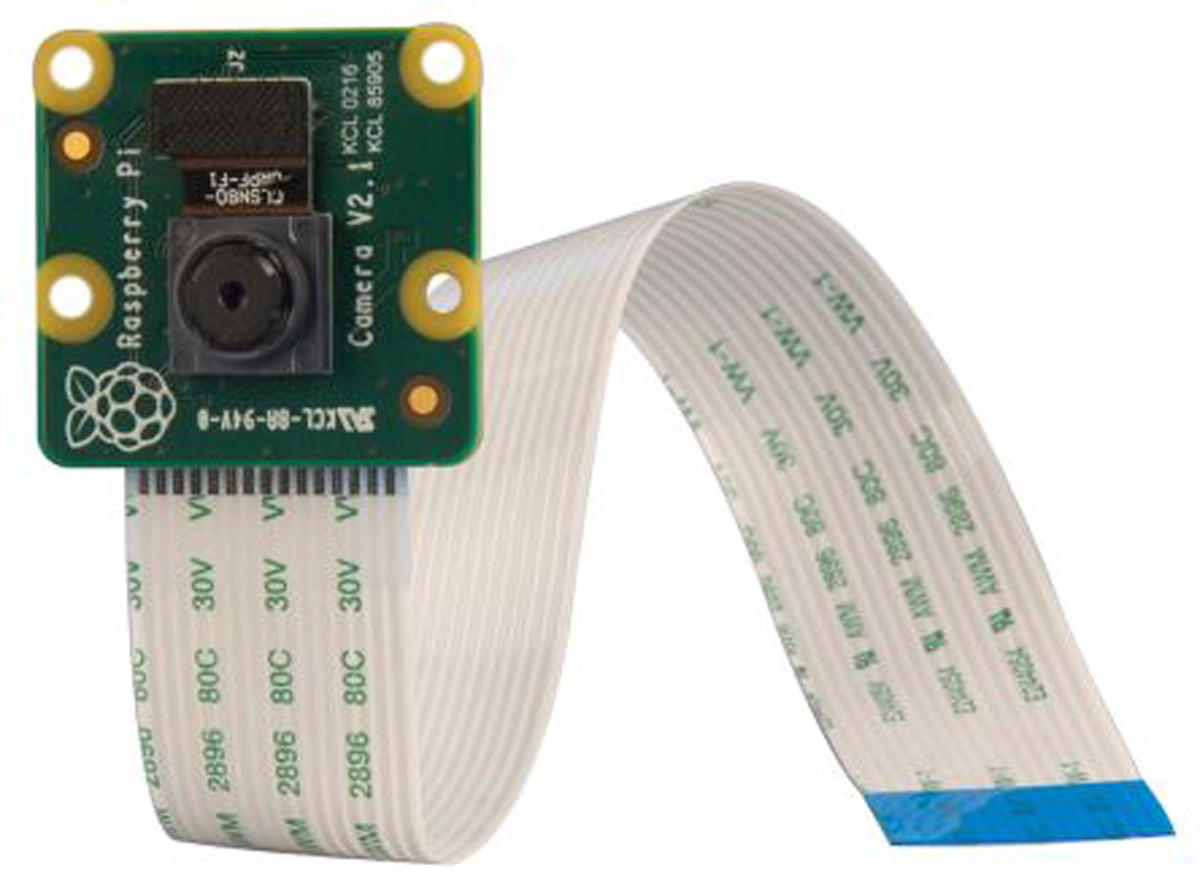
\includegraphics[width=3cm]{Images/Chap2/PiCameraV2.jpg} & An 8-megapixel camera that captures high-quality images with accurate color reproduction. \\
        \hline
        \textbf{Raspberry Pi Case with Fan} &
        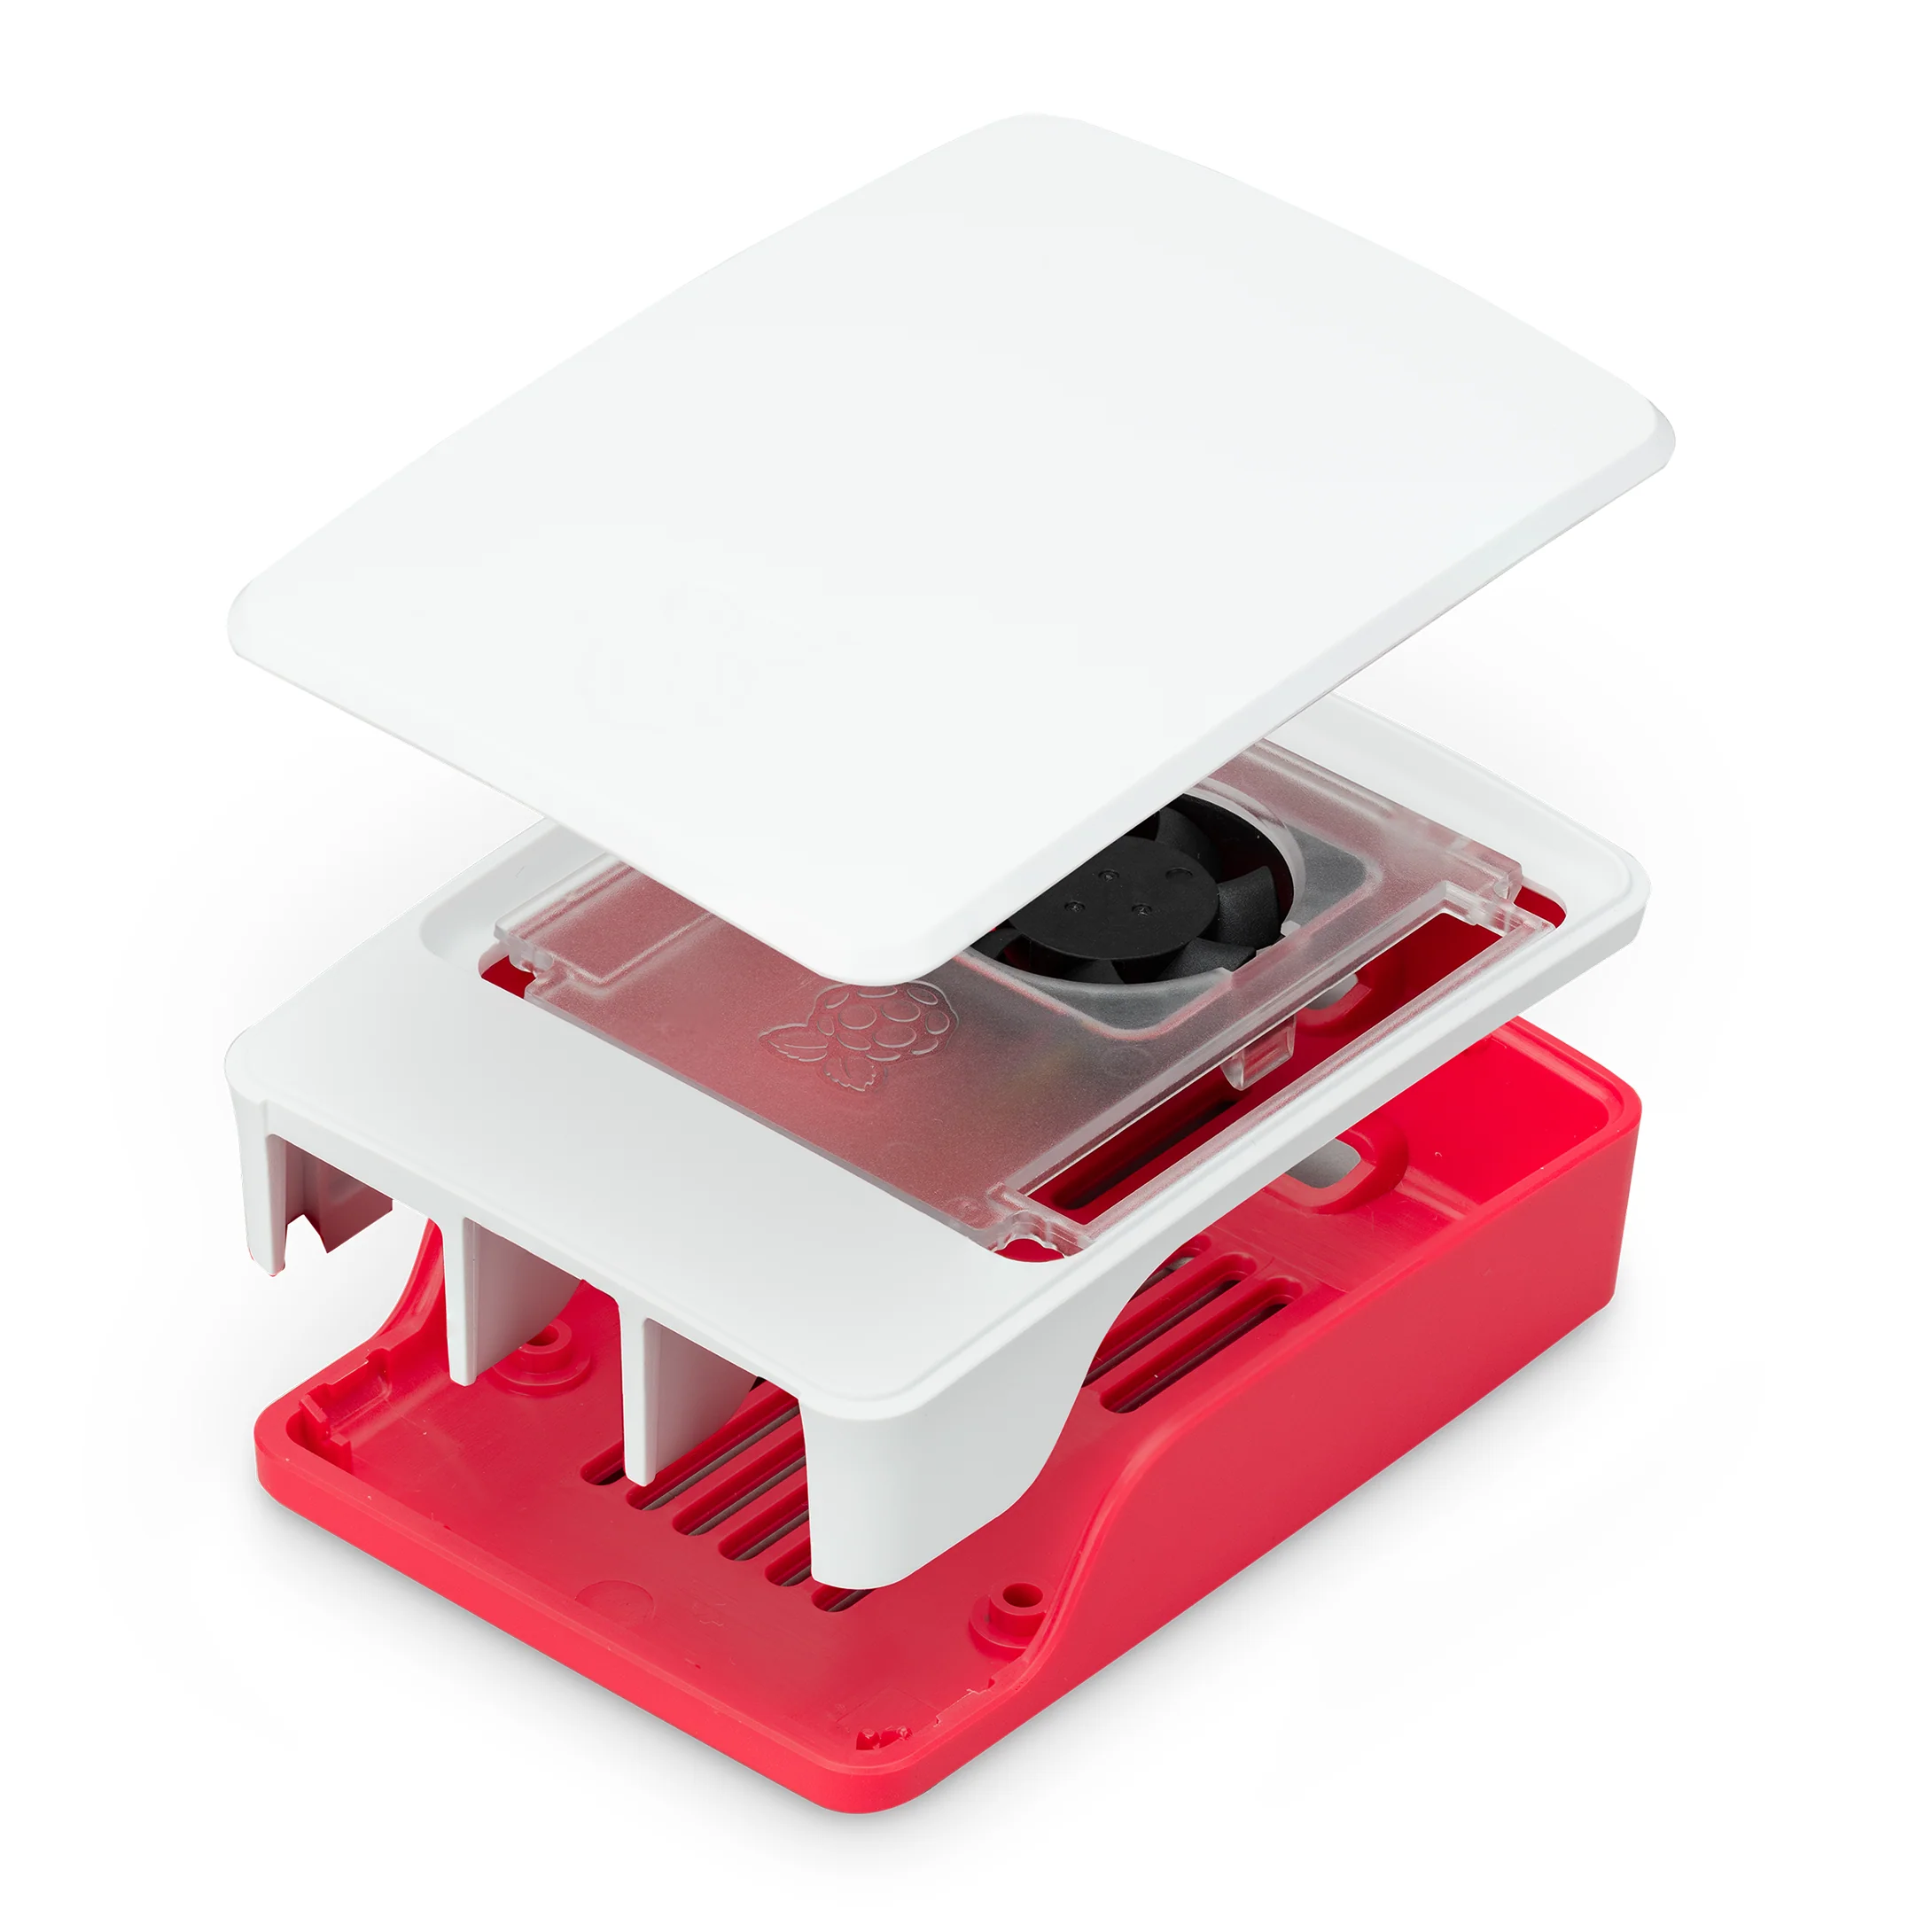
\includegraphics[width=3cm]{Images/Chap2/PiCaseFan.png} & A protective enclosure with an integrated fan to ensure stable performance. \\
        \hline
    \end{tabularx}
\end{table}
\section{Software Architecture}
The software architecture of the robotic sorting cell is built on a suite of specialized tools that integrate hardware control, design, simulation, and visualization. This approach ensures a streamlined workflow from conceptualization to implementation, with each software playing a distinct and crucial role.

\subsection{TIA Portal}
TIA Portal is a powerful and integrated software suite from Siemens that provides a single, unified environment for all automation tasks \hyperref[sec:bibliography]{[6]}. Its primary strength lies in its ability to centralize multiple engineering disciplines, including hardware configuration, PLC programming, and HMI design, into one platform. This integration was a key factor in its selection for this project, as it simplified the workflow, ensured data consistency across all components, and significantly reduced development time. The TIA Portal logo is shown in Figure \ref{fig:TIA_logo}.
\begin{figure}[H]
    \centering
    
\includegraphics[width=0.15\textwidth]{Images/Chap2/TIAPortal_logo.png}
    \caption{TIA Portal Logo}
    \label{fig:TIA_logo}
\end{figure}
\subsubsection{Key Advantages and Features}
The decision to use TIA Portal was driven by its numerous advantages that streamlined the development and commissioning of the automated sorting cell. The most significant benefits are outlined below:
\begin{itemize}
\item Integrated Engineering Environment: TIA Portal provides a single software platform for all automation tasks. This allows the entire project—from hardware setup and PLC logic to HMI design—to be managed within a unified environment, which eliminates the need for multiple software packages and ensures data consistency across all components;
\item Comprehensive Diagnostics and Troubleshooting: The software offers a powerful suite of diagnostic tools that provide real-time monitoring and fault analysis. This includes online functions to observe variable values, trace signal states, and identify network communication issues, which is critical for efficient debugging and commissioning;
\item Scalability and Reusability: TIA Portal's architecture is highly scalable, supporting a wide range of Siemens hardware, from small, modular PLCs to powerful, high-performance controllers. This flexibility allows for the easy expansion of a project;
\item Integrated Simulation: The platform provides a seamless connection to simulation software, such as S7-PLCSIM Advanced. This capability allows for virtual commissioning and testing of the control logic without physical hardware, significantly reducing development time and minimizing risks before deployment.
\end{itemize}

\subsubsection{Programming Languages and Communication Protocols}
TIA Portal supports a variety of programming languages that comply with the IEC 61131-3 standard, offering flexibility to developers. For this project, the primary languages used were Ladder Diagram and Structured Control Language. The supported languages include:
\begin{itemize}
\item Ladder Diagram (LAD): A graphical language that uses relay logic symbols, ideal for simple and sequential control;
\item Function Block Diagram (FBD): A graphical language that represents logic using interconnected function blocks;
\item Structured Control Language (SCL): A high-level, text-based language similar to Pascal, used for complex algorithms and data handling;
\item Statement List (STL): A low-level, text-based assembly-like language;
\item Sequential Function Chart (SFC): A graphical language used to model sequential processes.
\end{itemize}
In terms of communication, TIA Portal leverages a wide range of industry-standard protocols, including PROFINET, PROFIBUS, AS-Interface, and Ethernet/IP. While the platform supports this diverse array of communication standards, the primary protocol used for this project was PROFINET, a variant of industrial Ethernet, which enabled high-speed data exchange between the PLC, HMI, and other network devices.

\subsection{S7-PLCSIM Advanced V5.0}
S7-PLCSIM Advanced V5.0 is a powerful simulation tool that was used for virtual commissioning of the PLC program. It creates a virtual PLC that runs the exact same code as the physical hardware, allowing for comprehensive debugging and testing of the control logic without needing the real equipment. The S7-PLCSIM Advanced V5.0 logo is displayed in Figure \ref{fig:PLCSIM_logo}. This was particularly useful for verifying the complex state transitions of the GRAFCET sequence, as well as testing the synchronization between the virtual PLC and the robot's movements, saving significant time and resources during development. Annex \ref{fig:PLCSIM_workspace} shows the S7-PLCSIM Advanced Workspace for virtual commissioning.
\begin{figure}[H]
    \centering
    
\includegraphics[width=0.15\textwidth]{Images/Chap2/S7PLCSIMAdvanced_logo.jpg}
    \caption{S7-PLCSIM Advanced V5.0 Logo}
    \label{fig:PLCSIM_logo}
\end{figure}





\subsection{EPLAN}
EPLAN is an industry-standard software for creating professional electrical wiring diagrams and cabinet layouts. The EPLAN logo is presented in Figure \ref{fig:EPLAN_logo}. For this project, it was instrumental in designing the electrical schematics of the control cabinet and the pneumatic diagram. The use of EPLAN ensured that all wiring was logically organized, correctly documented, and compliant with safety standards. It also provided the necessary documentation for future maintenance and troubleshooting. The EPLAN workspace is shown in Annex \ref{fig:EPLAN_workspace}.
\begin{figure}[H]
    \centering
    
\includegraphics[width=0.2\textwidth]{Images/Chap2/EPLAN_logo.png}
    \caption{EPLAN Logo}
    \label{fig:EPLAN_logo}
\end{figure}


\subsection{Blender}
Blender is a versatile 3D computer graphics software that was used to develop a virtual model of the entire sorting cell\hyperref[sec:bibliography]{[7]}. The Blender logo is shown in Figure \ref{fig:Blender_logo}. This 3D model was crucial for visualizing the physical layout, optimizing the placement of the robot and conveyors, and simulating robot movements. The simulations in Blender were essential for verifying that the robot's reach was sufficient and that its motion paths were collision-free before any physical assembly took place, thereby mitigating potential design errors. The Blender workspace is shown in Annex \ref{fig:Blender_workspace}.
\begin{figure}[H]
    \centering
    
\includegraphics[width=0.2\textwidth]{Images/Chap2/Blender_logo.png}
    \caption{Blender Logo}
    \label{fig:Blender_logo}
\end{figure}


\subsection{WinCC Unified}
The HMI for the robotic sorting cell was developed using WinCC Unified, a powerful and modern platform seamlessly integrated within the TIA Portal framework. This technology represents a significant evolution from traditional HMI systems, offering key advantages that enhance the project's overall functionality and versatility.

Unlike conventional HMI systems (such as WinCC Comfort/Advanced), which typically rely on dedicated hardware panels or require specific runtime software to be installed on each client PC, WinCC Unified leverages modern web technologies. The HMI's interface is hosted on a central server, allowing it to be accessed directly through any standard web browser on a variety of devices. This capability is crucial, as it provides remarkable flexibility and portability, making the solution particularly impressive for public demonstrations and events. Figure \ref{fig:wincc_unified} illustrates the multi-platform capabilities of WinCC Unified.
\begin{figure}[H]
\centering
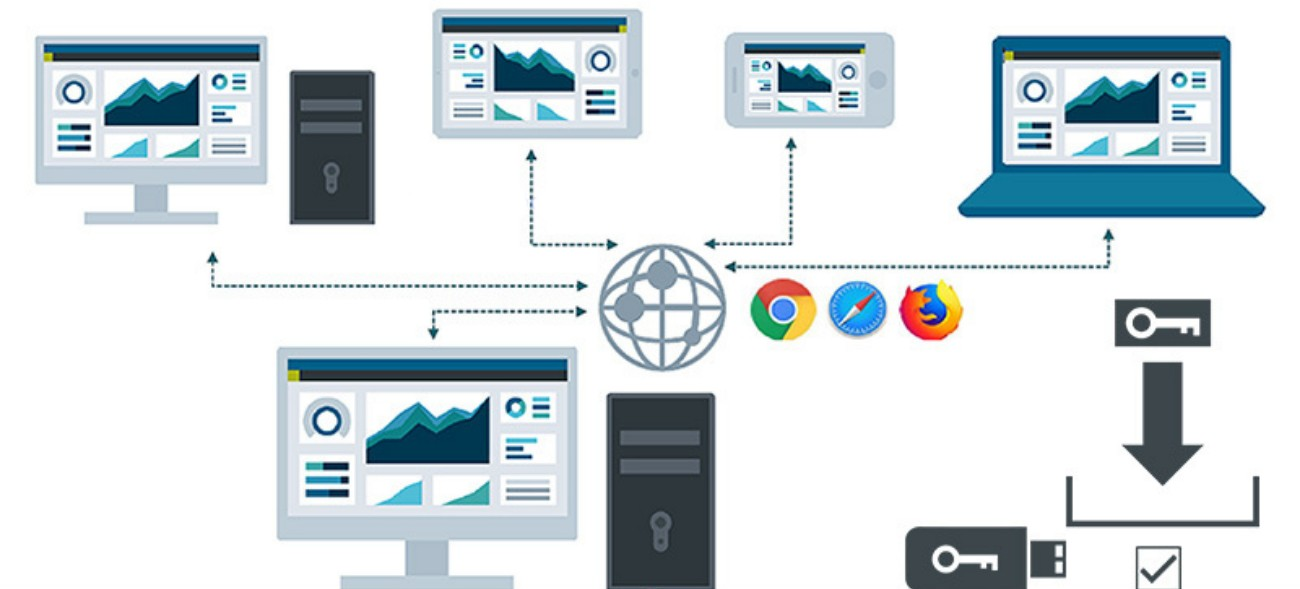
\includegraphics[width=0.7\textwidth]{Images/Chap3/unified.jpg}
\caption{WinCC Unified multi platform.}
\label{fig:wincc_unified}
\end{figure}
This web-based approach has several key benefits:
\begin{itemize}
\item Device Independence: The HMI can be viewed and controlled from a wide range of devices, including computers, tablets, and smartphones, without the need for additional client-side software.
\item Simplified Maintenance: Updates and changes to the HMI can be deployed centrally on the server, ensuring all clients are automatically using the latest version without individual updates.
\item Enhanced Accessibility: Operators and supervisors can monitor and interact with the system remotely from anywhere on the local network, improving operational oversight and responsiveness.
\end{itemize}

The project's HMI is deployed on a WinCC Unified Comfort Panel, but its browser-based design ensures that the interface is accessible from any client device, offering a scalable and future-proof solution.


\subsection{Python}
Python\hyperref[sec:bibliography]{[8]} is a high-level, interpreted programming language widely used in various applications, including computer vision, data analysis, and automation. Its simplicity and extensive libraries, such as \textbf{OpenCV}\hyperref[sec:bibliography]{[9]}, make it an ideal choice for the vision system in this project. Specifically, the Python script developed for this cell utilizes the OpenCV library for all image processing tasks.

\begin{figure}[H]
    \centering
    
\includegraphics[width=0.2\textwidth]{Images/Chap2/Python_logo.png}
    \caption{Python Logo.}
    \label{fig:Python_logo}
\end{figure}

The Python script is responsible for:
\begin{itemize}
    \item \textbf{Image Acquisition}:Capturing high-resolution images of the objects on the conveyor belt from the Raspberry Pi Camera Module;
    \item \textbf{Color Detection}: Analyzing the captured images to identify the color of each object using color space conversions and masking techniques;
    \item \textbf{Communication}: Sending the color information to the PLC via a TCP/IP or Ethernet connection, which then triggers the appropriate robot sequence for sorting.
\end{itemize}




\section{Conclusion}
This chapter provided a comprehensive overview of the automated sorting cell's foundational architecture, detailing its core hardware and software components. We explored the function of each element, from the central Programmable Logic Controller (PLC) and the Human-Machine Interface (HMI) to the KUKA robotic arm and the vision system. The discussion also covered the physical and logical cabinet layouts, establishing a robust framework for the system's safe and efficient operation. This thorough understanding of each component's role and its integration into the overall design is crucial for the successful implementation of the control logic detailed in the following chapters.










\chapter{Control System and Automation}

\section{Introduction}
This chapter will detail the automation logic and programming of the robotic sorting cell. It will cover the overall control philosophy, the programming environment, and the specific implementation details for the PLC and HMI.

\section{General Overview}
The control of the robotic sorting cell is handled by a Programmable Logic Controller (PLC), which acts as the central brain of the system. The PLC was chosen for its reliability, real-time processing capabilities, and industrial robustness. It continuously monitors the state of all sensors and, based on a pre-defined logic, sends commands to the actuators. The control philosophy prioritizes safety, sequential operation, and synchronization between all components, including the KUKA robot, conveyors, and pneumatic cylinders. This structured approach is fundamental to the system's efficient and predictable behavior.


\section{PLC Programming and Implementation}
This section details the programming of the PLC, covering the initial configuration, tag management, and the development of the main control logic.

\subsection{Hardware and Network Configuration}
The hardware and network configuration is the foundational step in a TIA Portal project, where the physical components are digitally modeled, and their communication links are established. This process ensures that all devices can interact seamlessly, forming a cohesive automation system. To make this process as clear as possible, it is broken down into a series of logical steps.

\begin{itemize}
\item Step 1: Component Selection

The first step involves selecting the appropriate hardware from TIA Portal's catalog, as shown in Annex \ref{fig:plc_selection} and Annex \ref{fig:hmi_selection}. This project utilized a physical SIMATIC S7-1212C PLC for the final application. However, for all simulation and virtual commissioning, a more advanced SIMATIC S7-1513-1 PN PLC was selected due to the requirements of the S7-PLCSIM Advanced software. This distinction between the physical and virtual hardware is crucial for a complete understanding of the development process. Additionally, the Human-Machine Interface (HMI) panel, which serves as the operator's primary control point, was also selected from the catalog to provide the necessary screen size and functionality for the sorting cell's interface. Specifically, the SIMATIC Unified Comfort Panel (MTP1200 Unified Comfort) was chosen;


\item Step 2: Network Setup

Once the devices (PLC and HMI) were added to the project, the network view within TIA Portal was used to establish communication links. This graphical interface allows for the virtual connection of devices, creating a logical representation of the physical network. The devices were interconnected via industrial Ethernet, which serves as the backbone for data exchange using the S7 communication protocol. The network topology is shown in Figure \ref{fig:network_setup};
\begin{figure}[H]
    \centering
    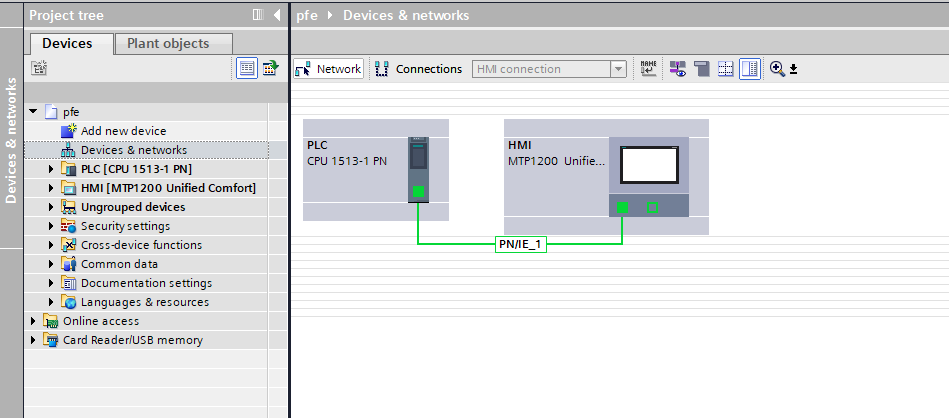
\includegraphics[width=0.9\textwidth]{Images/Chap3/connection.png}
    \caption{Network topology showing communication links between the PLC and HMI.}
    \label{fig:network_setup}
\end{figure}

\item Step 3: IP Address Configuration

A robust and reliable network is dependent on a consistent IP address schema. In this step, a unique IP address and a common subnet mask were assigned to each device to ensure seamless communication. The physical PLC was assigned the address 192.168.0.1 and the HMI was set to 192.168.0.2. The subnet mask for all devices was configured as 255.255.255.0, establishing that they all reside on the same network segment and can exchange data without any routing issues. The IP address configuration for network devices is shown in Figure \ref{fig:ip_configuration}.
\begin{figure}[H]
    \centering
    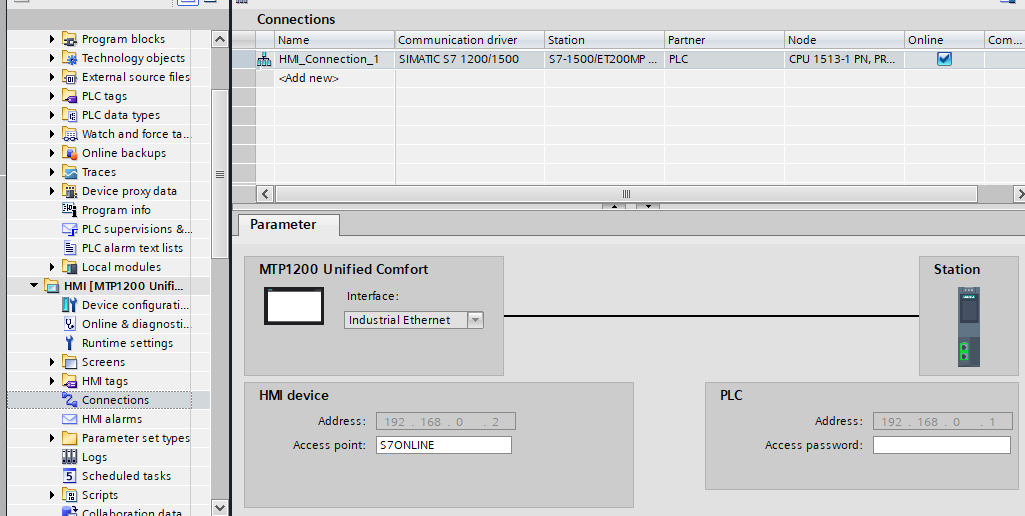
\includegraphics[width=0.9\textwidth]{Images/Chap3/Ips.png}
    \caption{IP address configuration for network devices.}
    \label{fig:ip_configuration}
\end{figure}

\end{itemize}

\subsection{Data Management and Tagging}
Effective data management is crucial for a well-structured and maintainable program. All I/O signals and internal variables are organized into Data Blocks (DBs) for a clear and logical structure.

\subsubsection{Input and Output Tags}
All physical inputs and outputs are mapped to their corresponding addresses in a dedicated InputDB and OutputDB, as shown in Figure \ref{fig:input_tags} and Figure \ref{fig:output_tags}. This makes the program hardware-independent, as the main logic can reference these tags without being directly tied to physical addresses.
\begin{figure}[H]
\centering
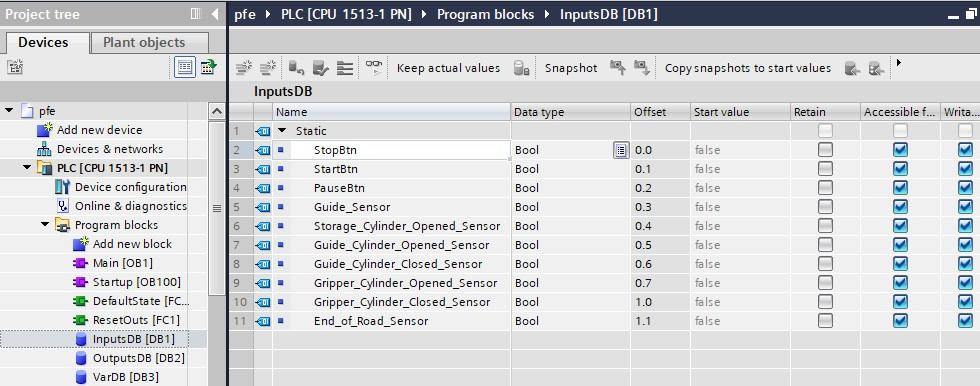
\includegraphics[width=1\textwidth]{Images/Chap3/tags_inputs_db.jpg}
\caption{Mapping physical inputs to symbolic tags.}
\label{fig:input_tags}
\end{figure}
\begin{figure}[H]
\centering
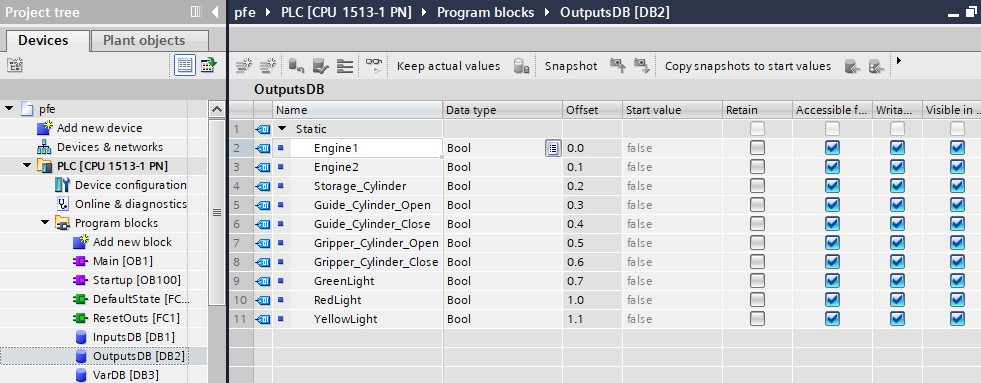
\includegraphics[width=1\textwidth]{Images/Chap3/tags_outputs_db.jpg}
\caption{Mapping physical outputs to symbolic tags.}
\label{fig:output_tags}
\end{figure}

\subsubsection{Internal tags}
A key part of this structured approach was the use of a dedicated set of internal tags, from \textbf{X0 to X13}, to track the active steps of the GRAFCET sequence. This direct mapping between the GRAFCET steps and the PLC tags made the implementation of the sequential logic straightforward and easy to debug.

The following figure provides a visual overview of the tag management for the GRAFCET steps, showing their direct mapping to the sequential logic.
\begin{figure}[H]
    \centering
    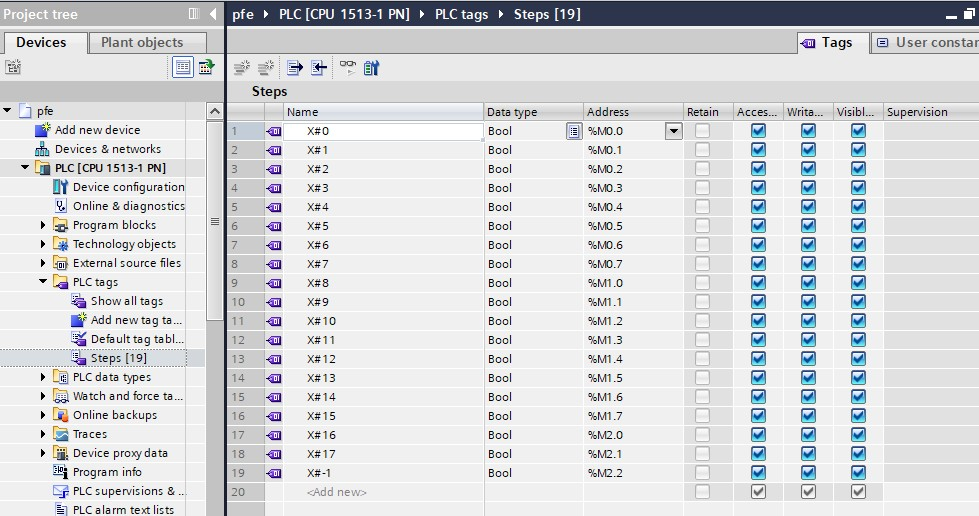
\includegraphics[width=1\textwidth]{Images/Chap3/tags_steps.jpg}
    \caption{TIA Portal screenshot showing the tags for the GRAFCET steps (X0-13).}
    \label{fig:tags_steps}
\end{figure}
\subsubsection{State Variables}
This section defines the key internal state variables used by the program. These variables are stored in a dedicated Global Data Block (VarDB), which allows them to be accessed from any part of the program. They include the operational status, sequential steps, and actuator control variables, as detailed below:

\begin{itemize}
\item Status Variable (VarDB.Status)
This variable controls the overall operational mode of the cell, dictating its behavior during the cycle.
\begin{table}[H]
    \centering
    \begin{tabular}{|p{0.15\textwidth}|p{0.35\textwidth}|}
        \hline
        \textbf{Value} & \textbf{State Description} \\
        \hline
        
        0 & Stop Mode \\
        \hline
        1 & Running Mode \\
        \hline
        2 & Pause Mode \\
        \hline
        3 & Maintenance Mode \\
        \hline
        4 & Resetting Mode \\
        \hline
    \end{tabular}
\end{table}

\item Robot Status Variable (VarDB.RobotStatus)
This variable indicates the current status of the KUKA robot, allowing the PLC to know if the robot is waiting or moving.
\begin{table}[H]
    \centering
    \begin{tabular}{|p{0.15\textwidth}|p{0.35\textwidth}|}
        \hline
        \textbf{Value} & \textbf{State Description} \\
        \hline
        0 & At Home Position \\
        \hline
        1 & Moving \\
        \hline
        2 & Ready \\
        \hline
        3 & Paused \\
        \hline
    \end{tabular}
\end{table}

\item Robot Position Variable (VarDB.RobotPos)
An integer value that sends the robot to a specific position. The PLC sends one of these values to the robot to command it to move to a defined location.
\begin{table}[H]
    \centering
    \begin{tabular}{|p{0.15\textwidth}|p{0.35\textwidth}|}
        \hline
        \textbf{Value} & \textbf{State Description} \\
        \hline
        0 & Home Position \\
        \hline
        1 & Pick-up Position \\
        \hline
        2 & Red Bin Position \\
        \hline
        3 & Green Bin Position \\
        \hline
        4 & Blue Bin Position \\
        \hline
    \end{tabular}
\end{table}

\item Cube Color Variable (VarDB.CubeColor)
This integer value represents the color of the cube detected by the vision system, a key input for the sorting logic, and is set by the Raspberry Pi after it processes the vision data.
\begin{table}[H]
    \centering
    \begin{tabular}{|p{0.15\textwidth}|p{0.35\textwidth}|}
        \hline
        \textbf{Value} & \textbf{State Description} \\
        \hline
        1 & Red Cube \\
        \hline
        2 & Green Cube \\
        \hline
        3 & Blue Cube \\
        \hline
        0 & No Cube Detected \\
        \hline
    \end{tabular}
\end{table}

\item Cylinder Control Variables (VarDB.GuideState / VarDB.GripperState)
These variables control the pneumatic cylinders, which are used to guide the cubes and operate the gripper. They share a similar logic where an integer value dictates the state of the actuator.

   \begin{table}[H]
        \centering
        \begin{tabular}{|p{0.15\textwidth}|p{0.35\textwidth}|}
            \hline
            \textbf{Value} & \textbf{State Description} \\
            \hline
            1 & Idle \\
            \hline
            2 & Open Cylinder \\
            \hline
            4 & Close Cylinder \\
            \hline
        \end{tabular}
    \end{table}

\item Cube Counter Variables
These integer variables are used to track the number of cubes sorted, providing essential feedback on the system's performance.
\begin{itemize}
    \item VarDB.BlueCubesCounter
    \item VarDB.GreenCubesCounter
    \item VarDB.RedCubesCounter
\end{itemize}

\end{itemize}

The main state variables defined in the Global Data Block are shown in Figure \ref{fig:tags}.
\begin{figure}[H]
\centering
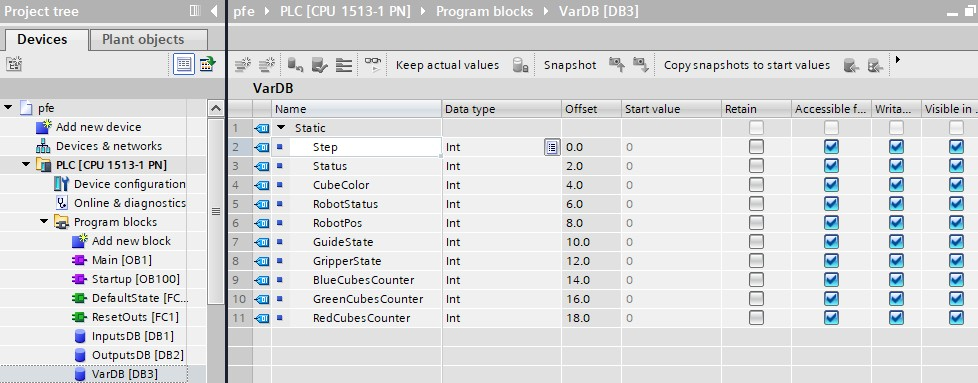
\includegraphics[width=1\textwidth]{Images/Chap3/tags_variables_db.jpg}
\caption{The main state variables defined in the Global Data Block.}
\label{fig:tags}
\end{figure}


\subsection{GRAFCET}
To design and visualize the sequential control logic, a GRAFCET (Graph for Step-by-Step Control) approach was used. GRAFCET is a graphical language that simplifies complex automation sequences by breaking the process down into a series of steps and transitions. Each step represents a state of the system where specific actions occur, while each transition defines the conditions that must be met to move to the next step.

Transitions between these steps are triggered by logical conditions, such as sensor signals confirming a part's presence, operator inputs from the HMI, or completion signals from the robotic arm. This method ensures a clear, visual representation of the entire process, making it easy to understand, debug, and modify the control logic.

The final GRAFCET, as shown in Annex \ref{fig:grafcet_logic}, was designed to manage a single, complete sorting cycle. This design decision, while limiting continuous operation, was necessary due to the constraints of the simulation environment, where automated sensor activation for a continuous loop could not be realistically emulated. The diagram presents the primary operational sequence, which handles the sorting process from start to finish. A 3D representation of the automated sorting cell with key components is also shown in Annex \ref{fig:cell_3d_view_annotated}.



\subsection{Programming Languages and Fundamental Blocks}
For this project, the primary language used was Ladder Diagram (LAD). Its graphical, relay-logic format was ideal for implementing and troubleshooting the sequential control logic. Within LAD, the control logic is built using a combination of fundamental blocks. The following are the most important blocks used in this project:

\subsubsection{Comparison Blocks}

Functionality: These blocks are used to compare two values and return a Boolean result (TRUE or FALSE). They are essential for creating conditional logic within the program. The images show a comparison for both equality (==) and inequality (<>), as shown in Figure \ref{fig:comparison_blocks}.

Inputs and Outputs: Comparison blocks take two numerical inputs (e.g., from an integer variable or a constant value) and provide a single Boolean output.

When to Use: These blocks are used to check the status of a variable before allowing a specific action to proceed. For instance, comparing the CubeColor variable to a specific integer to determine the type of object, or checking the RobotStatus variable for a specific value to confirm the robot is ready.
\begin{figure}[H]
\centering
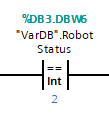
\includegraphics[width=0.2\textwidth]{Images/Chap3/tags_equals.png}
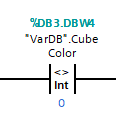
\includegraphics[width=0.2\textwidth]{Images/Chap3/tags_different.png}
\caption{Comparison blocks for equality and inequality.}
\label{fig:comparison_blocks}
\end{figure}

\subsubsection{Move Blocks}
Functionality: The MOVE block transfers the value from its input (IN) to its output (OUT). A typical MOVE block in Ladder Diagram is shown in Figure \ref{fig:move_block_lad}.

Inputs and Outputs: The input can be a numerical value, a constant, or a variable address. The output is a variable address where the value will be stored. The block also has a Boolean enable input (EN) and output (ENO) to control its execution.


When to Use: This block is used to set the value of a variable. A common application in this project is to move a new State number to the VarDB.Status tag.

\begin{figure}[H]
    \centering
    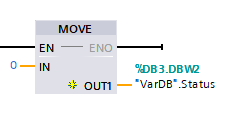
\includegraphics[width=0.4\textwidth]{Images/Chap3/move_block.png}
    \caption{A typical MOVE block in Ladder Diagram.}
    \label{fig:move_block_lad}
\end{figure}

\subsubsection{Set/Reset (SR) Blocks}
Functionality: The Set block forces a Boolean output to a TRUE state, while the Reset block forces it to a FALSE state.

When to Use: These blocks are used for direct control of output bits, such as a solenoid or a motor. The Set and Reset blocks for controlling outputs are shown in Figure \ref{fig:set_reset_blocks}. The two images show how an output can be Set or Reset to control the state of the Storage Cylinder.

 \begin{figure}[H]
    \centering
    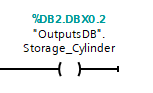
\includegraphics[width=0.3\textwidth]{Images/Chap3/set_block.png}
    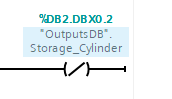
\includegraphics[width=0.31\textwidth]{Images/Chap3/reset_block.png}
    \caption{Set and Reset blocks for controlling outputs.}
    \label{fig:set_reset_blocks}
\end{figure}



\subsubsection{SR Flip-Flop}
Functionality: The SR (Set/Reset) flip-flop is a memory element. When the S input is activated, the output Q is set to TRUE. It remains TRUE even if the S input deactivates. The output is only reset to FALSE when the R input is activated. If both inputs are active at the same time, the R input has priority. The block for this logic is shown in \textbf{Figure \ref{fig:sr_flip_flop}}.

Inputs and Outputs: It has two Boolean inputs, S (Set) and R1 (Reset), and a single Boolean output, Q.

When to Use: This block is fundamental for implementing sequential logic. It is used to activate and hold the state of a step in the GRAFCET sequence until a new transition condition is met, such as setting the X\#3 bit to TRUE and holding it until the next step is ready.

\begin{figure}[H]
\centering
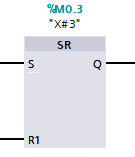
\includegraphics[width=0.2\textwidth]{Images/Chap3/sr_flip_flop.png}
\caption{The SR flip-flop block for sequential logic.}
\label{fig:sr_flip_flop}
\end{figure}

\subsubsection{Single-Shot Pulse (P\_TRIG)}
The P\_TRIG block generates a one-scan pulse on the rising edge of its input signal. This is crucial for triggering an action only once when a condition becomes true, preventing continuous execution that could lead to unexpected behavior. The P\_TRIG block is shown in \textbf{Figure \ref{fig:p_trig}}.
\begin{figure}[H]
\centering
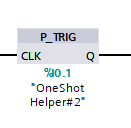
\includegraphics[width=0.2\textwidth]{Images/Chap3/trig.png}
\caption{The P\_TRIG block for single-scan pulses.}
\label{fig:p_trig}
\end{figure}
\subsection{Subroutines}
To simplify the main program loop and promote code reusability, several key functions were developed. These subroutines encapsulate specific, repeating logic, allowing the Main block to be a high-level overview of the entire process. This modular approach significantly improves readability, reduces the chance of errors, and makes the program easier to modify in the future. The process of adding a function block in TIA Portal is shown in \textbf{Figure \ref{fig:function_block}}.
\begin{figure}[H]
\centering
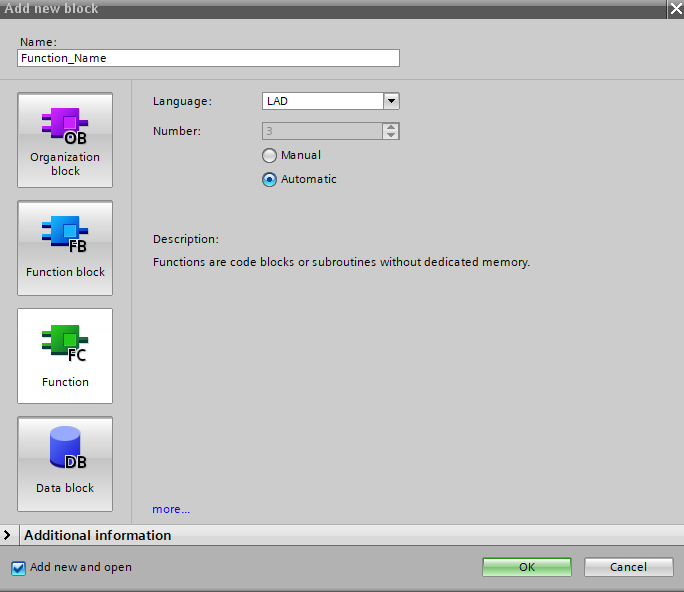
\includegraphics[width=0.5\textwidth]{Images/Chap3/Function.png}
\caption{Adding a function block in TIA Portal.}
\label{fig:function_block}
\end{figure}
\begin{itemize}
\item The DefaultState Function (FC2):
The DefaultState function is a crucial subroutine that ensures all key variables and outputs are reset to a safe, initial state. This function is called at the beginning of the program's Resetting Mode and whenever a cycle needs to be restarted. Its purpose is to guarantee a consistent and predictable starting point for every run, which is fundamental for system reliability and safety.

This function uses a series of MOVE blocks to set the values of the main state variables to their default safe values. As shown in \textbf{Figure \ref{fig:defaultstate}}, this includes resetting the Guide State, Gripper State, Robot Status, and Cube Color to a safe, initial value.

\begin{figure}[H]
    \centering
    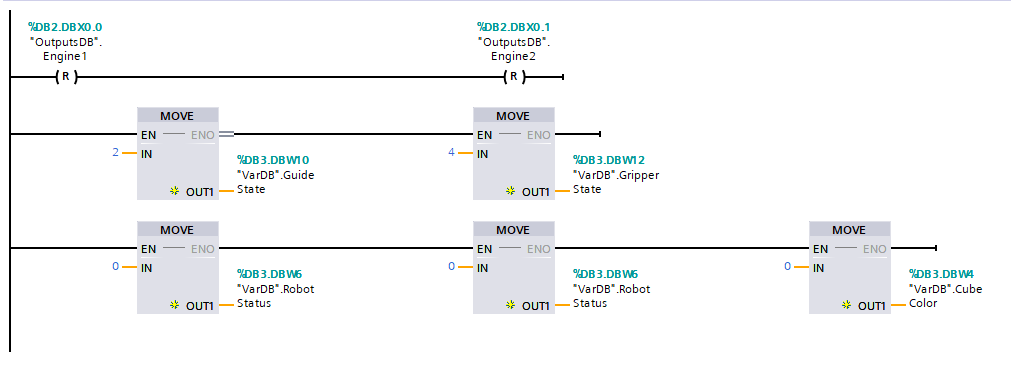
\includegraphics[width=0.9\textwidth]{Images/Chap3/DefaultState.png}
    \caption{Ladder logic for the DefaultState function.}
    \label{fig:defaultstate}
\end{figure}

\item The ResetOuts Function (FC1)
The ResetOuts function is a dedicated subroutine for turning off all outputs. It is called at the end of a cycle or when a fault is detected to ensure that no actuators are left active. This is a critical safety measure that prevents unintended movements or actions.

The function uses MOVE blocks to set the outputs to 0, effectively deactivating them. \textbf{Figure \ref{fig:resetouts}} shows this function resetting outputs for the motors, storage cylinder, gripper, and guide cylinder. The separation of this logic into a dedicated function ensures that the process of shutting down the system is both thorough and easy to manage from anywhere in the main program.

    \begin{figure}[H]
        \centering
        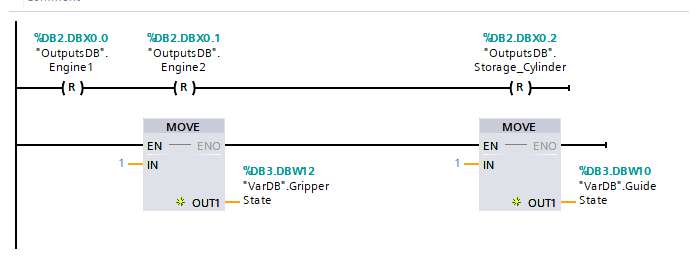
\includegraphics[width=1\textwidth]{Images/Chap3/ResetOuts.png}
        \caption{Ladder logic for the ResetOuts function.}
        \label{fig:resetouts}
    \end{figure}
\end{itemize}

\subsection{Sequential and Actuator Logic}
The core of the program is divided into input logic, which handles step transitions, and output logic, which controls actuators based on the current step. This separation simplifies development and debugging.

The input logic is the engine of the sequential program, with each transition represented by a separate network. As shown in \textbf{Figure \ref{fig:move_block_new}}, an SR flip-flop advances the program from the initial state (X\#0) to the next (X\#1). The flip-flop is set when the start button is pressed in the initial state and reset by the stop button or by advancing to a new step. Once set, a Move block writes the new step number to VarDB.Step.
\begin{figure}[H]
\centering
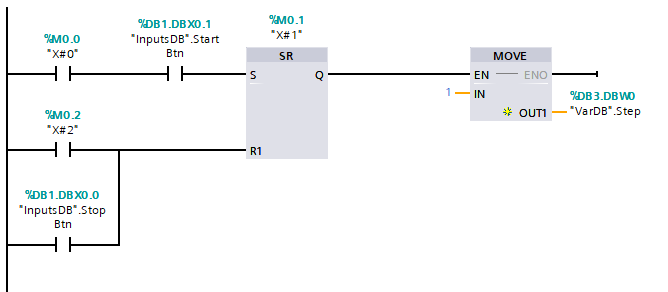
\includegraphics[width=1\textwidth]{Images/Chap3/network1.png}
\caption{Initial step logic with an SR flip-flop and a Move block.}
\label{fig:move_block_new}
\end{figure}

The output logic is straightforward. For each actuator, a dedicated network controls its state. \textbf{Figure \ref{fig:storage_cylinder_logic}} shows the logic for the Storage Cylinder, which extends when the program is in step (X\#1) and the status is set to Running (VarDB.Status = 1).
\begin{figure}[H]
\centering
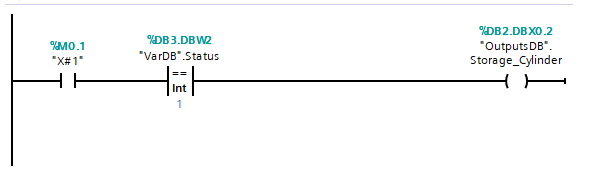
\includegraphics[width=1\textwidth]{Images/Chap3/network17.png}
\caption{Sample output logic for the Storage Cylinder.}
\label{fig:storage_cylinder_logic}
\end{figure}

The logic for returning the system to its initial state is shown in \textbf{Figure \ref{fig:tags_steps_home}}. This network is responsible for a complete system reset based on sensor checks. An SR flip-flop is used to manage this state. Its set input is activated by a combination of the (X\#1) step being active and all sensors confirming that the cylinders are in their home positions. Once these conditions are met, a Move block writes the value 0 to VarDB.Step, returning the system to the initial state (X\#0). The flip-flop is reset only by the (X#1) step, ensuring the system can be automatically reset.
\begin{figure}[H]
\centering
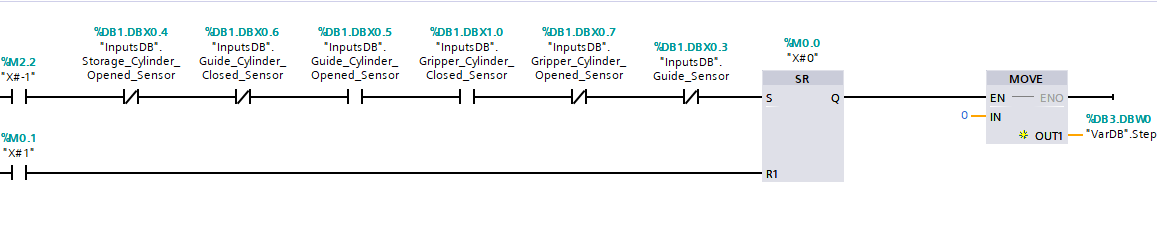
\includegraphics[width=1\textwidth]{Images/Chap3/network21.png}
\caption{Transition logic for resetting the system to the home position.}
\label{fig:tags_steps_home}
\end{figure}

More complex logic, such as sending commands to the KUKA robot, is handled by a single-shot pulse. As shown in \textbf{Figure \ref{fig:robot_logic}}, a P\_TRIG block is triggered once when the system enters step (X\#7) and the VarDB.Status is 1. This pulse then triggers a sequence of three Move blocks to command the robot's position and gripper state.
\begin{figure}[H]
\centering
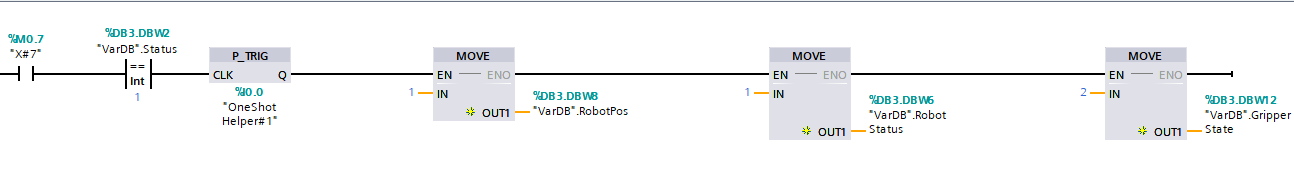
\includegraphics[width=1\textwidth]{Images/Chap3/network111.png}
\caption{Logic for sending commands to the KUKA robot.}
\label{fig:robot_logic}
\end{figure}

The logic for the guide cylinder, shown in \textbf{Figure \ref{fig:guide_cylinder_logic}}, operates with three distinct states controlled by VarDB.GuideState: 1 for idle, 2 for extend, and 4 for close. The logic incorporates sensor checks to prevent over-extension or over-retraction. This same logic, with minor adjustments for specific sensor and actuator tags, is also used for the gripper cylinder.
\begin{figure}[H]
\centering
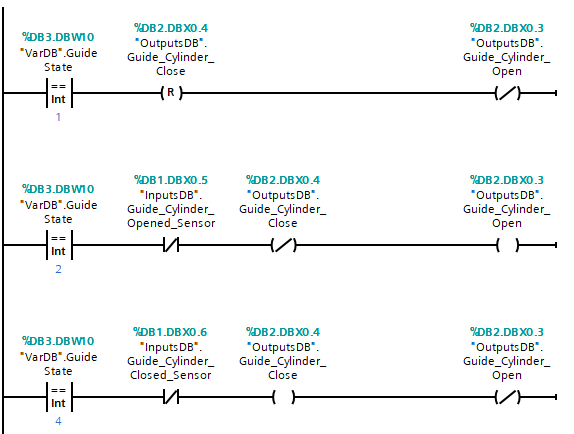
\includegraphics[width=0.8\textwidth]{Images/Chap3/network_guide_cylinder_logic1.png}
\caption{Logic for controlling the guide cylinder.}
\label{fig:guide_cylinder_logic}
\end{figure}

The last main block of logic handles the sorting process, as shown in \textbf{Figure \ref{fig:sorting_logic}}. When the system is in Running mode (VarDB.Status = 1) and VarDB.Step is equal to 9, a single pulse is generated by the P\_TRIG block. The first Move block then writes 1 to VarDB.RobotStatus, indicating the robot is ready to move to the pick-up position. A series of conditional branches then check the value of VarDB.CubeColor. Based on the color (1 for red, 2 for green, 3 for blue), a Move block commands the robot to move to the correct sorting position and a counter for that color is incremented.
\begin{figure}[H]
\centering
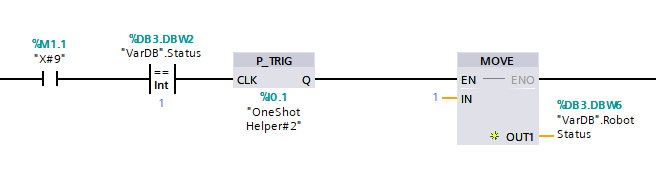
\includegraphics[width=0.8\textwidth]{Images/Chap3/network_sorting_logic1.png}
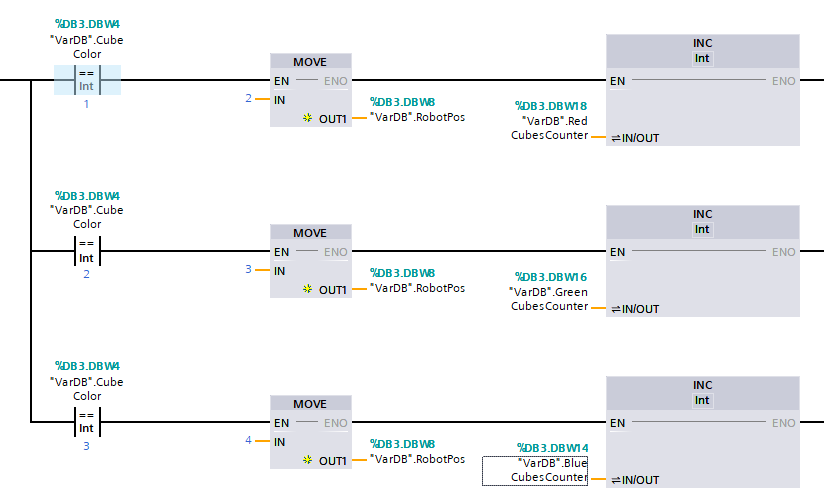
\includegraphics[width=0.8\textwidth]{Images/Chap3/network_sorting_logic2.png}
\caption{Logic for the sorting process.}
\label{fig:sorting_logic}
\end{figure}

\section{HMI Programming and Design}
This section focuses on the development of the Human-Machine Interface (HMI) using the TIA Portal framework. It will cover the creation of graphical user interface screens, the design of interactive elements like buttons and indicators, and the configuration of communication links to the PLC.

\subsection{Screen Navigation and Layout}
This section will detail the purpose and layout of the two main screens that were designed for system operation and maintenance.

\subsubsection{Production Screen}
The Production Screen serves as the primary operational interface for the sorting cell. Its design is focused on providing the operator with a clear and concise overview of the machine's status and real-time production data. The screen layout is intuitive, with key control buttons and status indicators located in a central position.

As shown in \textbf{Figure \ref{fig:production_screen}}, the screen includes:
\begin{itemize}
\item Cube Counters: Three distinct counters display the total number of red, blue, and green cubes sorted. These counters are linked to integer tags in the PLC and update in real-time, providing immediate feedback on the sorting process;
\item Status Indicators: The "Machine Status" and "Robot Status" boxes provide a visual indication of the system's current state. The text and color of these boxes change dynamically based on the corresponding integer values from the PLC, allowing the operator to quickly assess the machine's condition;
\item Control Buttons: Large, clearly labeled buttons for "Start," "Stop," and "Pause" allow the operator to control the main operational cycle. A key safety feature implemented is that these buttons are only enabled or disabled based on the machine's current state. For example, the "Start" button is only accessible when the machine is in the Stop or Pause mode, preventing accidental activation.
\end{itemize}
The "Maintenance" button provides a direct navigation link to the dedicated maintenance screen.

\begin{figure}[H]
\centering
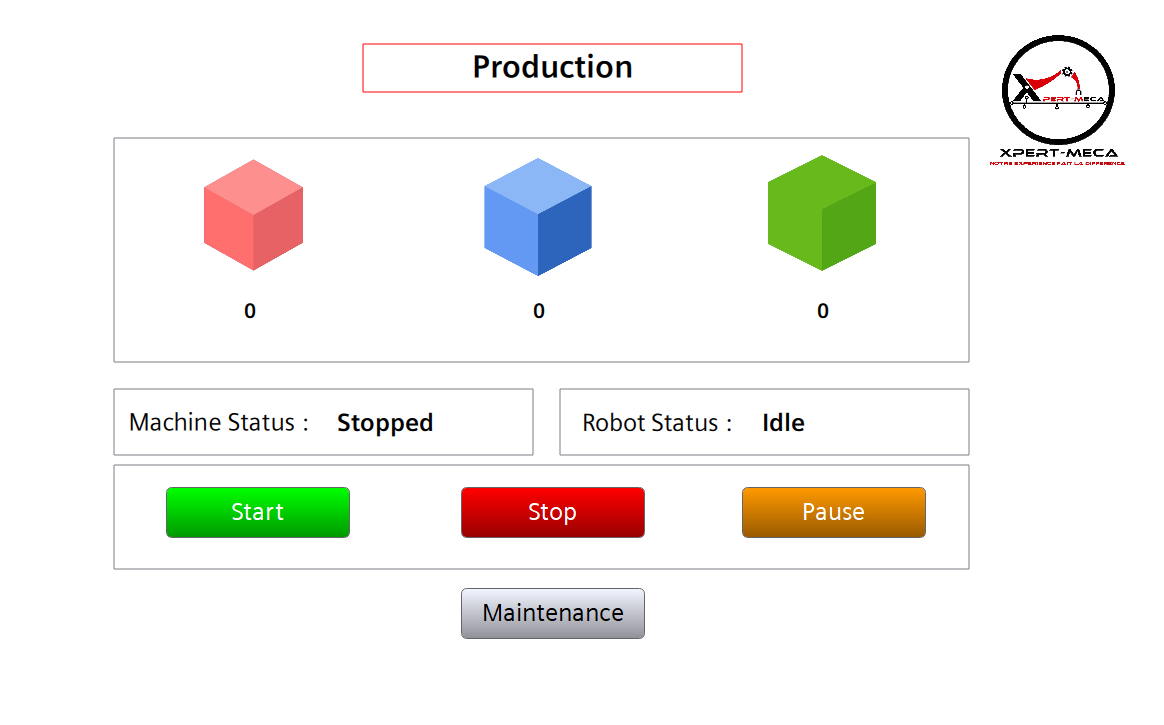
\includegraphics[width=0.8\textwidth]{Images/Chap3/production_screen.png}
\caption{The Production Screen of the HMI.}
\label{fig:production_screen}

\end{figure}

\subsubsection{Maintenance Screen}
The Maintenance Screen is a dedicated interface for troubleshooting, manual control, and detailed diagnostics. Unlike the Production Screen, which is designed for quick operation, the Maintenance Screen provides a comprehensive overview of the system's internal state and allows the operator to manually override outputs and simulate inputs. This mode is critical for commissioning and debugging the system. The overall layout is shown in \textbf{Figure \ref{fig:maintenance_screen}}.

The screen is organized into distinct functional areas:
\begin{itemize}
\item Status Display: This section provides granular, real-time status information, including the "Machine State," "Robot State," "Current Step" in the PLC program, and the "Cube Color" detected by the vision system;
\item Input Simulation Buttons: A key feature is the ability to manually trigger simulated inputs. This array of buttons, corresponding to physical sensors (e.g., "End of Road Sensor") and start/stop buttons, allows technicians to test the PLC logic without requiring the physical presence of parts or the activation of real-world sensors;
\item Output Visualization and Control: This area provides a visual representation of the system's key outputs. The operator can see the status of motors and cylinders and, crucially, can manually control them by toggling switches and pressing buttons to diagnose issues or perform manual maneuvers.
\end{itemize}
The "Back" button at the top left allows for seamless navigation back to the Production screen.

\begin{figure}[H]
\centering
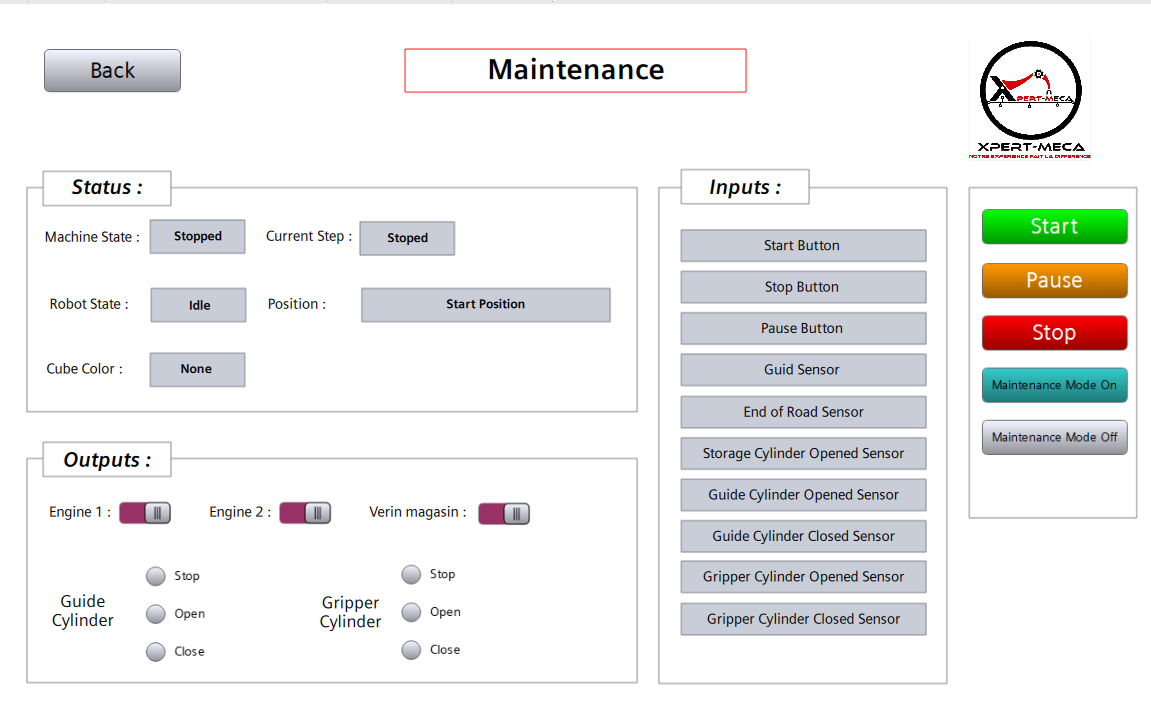
\includegraphics[width=1\textwidth]{Images/Chap3/maintenance_screen.png}
\caption{The Maintenance Screen of the HMI.}
\label{fig:maintenance_screen}
\end{figure}


\subsection{Dynamic Status Indicators}
The status indicators on the HMI screens are not static, they change their text and color based on the machine’s real-time state. This dynamic feedback is crucial for providing operators with immediate visual cues. This effect is achieved by linking the display element's properties to a PLC tag and configuring a range of values.

\subsubsection{Linking a Variable to a Text String}
This process allows a numerical value from the PLC to be displayed as descriptive text on the HMI. For example, a PLC variable with the value 1 can be shown as "RUNNING."

\begin{enumerate}
\item Create the Text List: In the HMI project tree in TIA Portal, navigate to HMI Tags Text and graphic lists and add a new list. This is the central repository for defining the text associated with each value.
\item Define List Entries: In the new text list, add entries for each state. Each entry requires a value and a corresponding text string. For the "Machine Status" indicator, we would define entries such as:
\begin{itemize}
\item Value 0: Text "Stopped";
\item Value 1: Text "Running";
\item Value 2: Text "Paused";
\item Value 3: Text "Maintenance";
\item Value 4: Text "Resetting".
\end{itemize}
\textbf{Figure \ref{fig:status_text}} shows how this is configured in TIA Portal.
\begin{figure}[H]
\centering
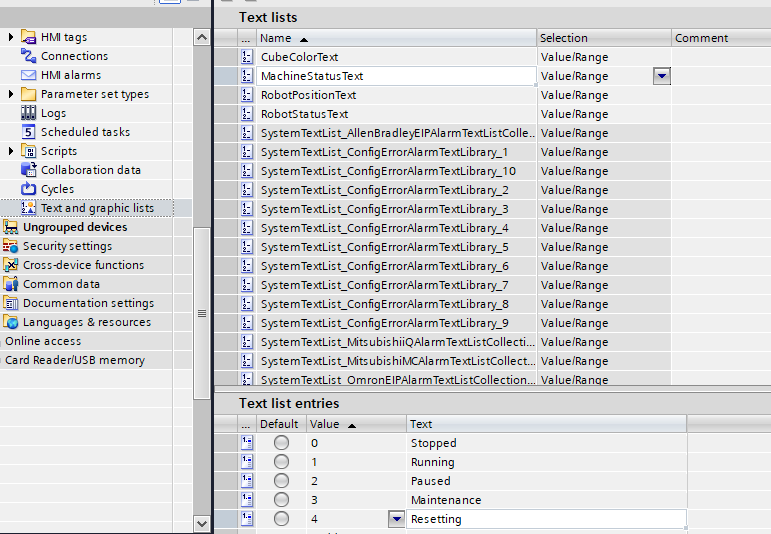
\includegraphics[width=0.8\textwidth]{Images/Chap3/status_text.png}
\caption{HMI configuration for a status text list that links a variable's value to a text string.}
\label{fig:status_text}
\end{figure}
\item Link the Text Box: On the HMI screen, place a text box or an I/O field. In its properties, navigate to General > Text and link it to the PLC tag that represents the machine's status (e.g., VarDB.MachineStatus). Then, under Text list, select the list you just created. The HMI will now automatically display the correct text based on the tag's current value. \textbf{Figure \ref{fig:text_list_link}} shows how to link the text box to the PLC variable.
\begin{figure}[H]
\centering
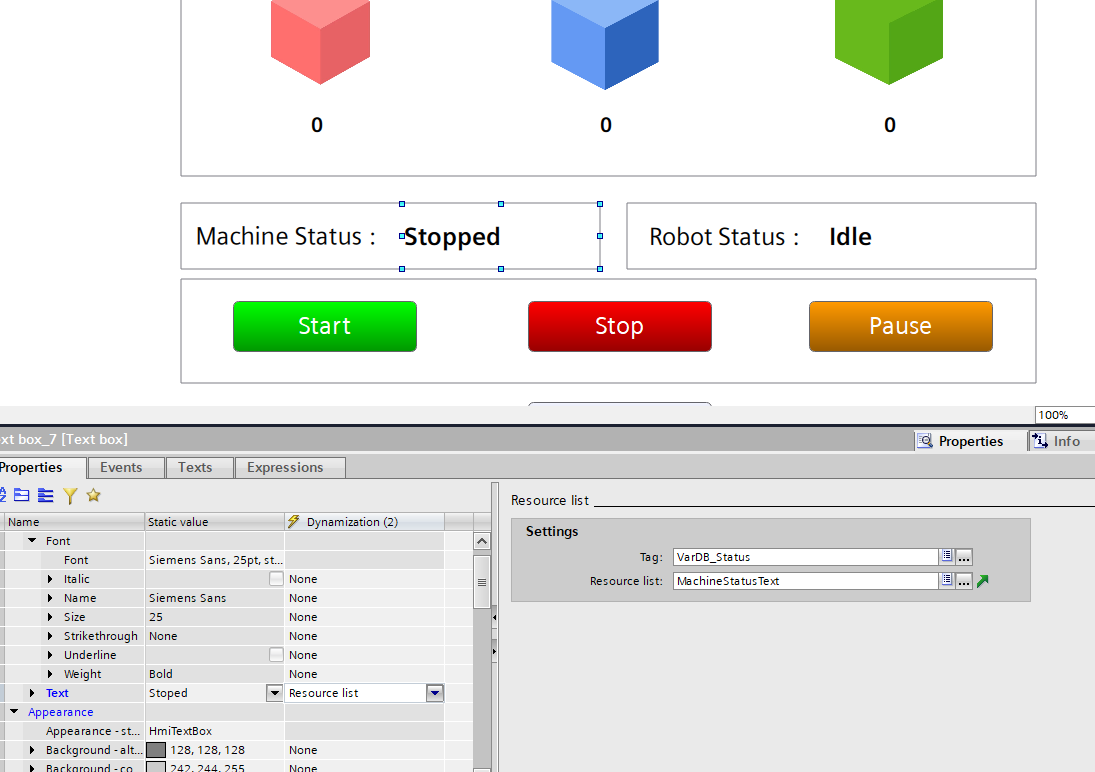
\includegraphics[width=1\textwidth]{Images/Chap3/link.png}
\caption{HMI properties panel for linking a text box to a PLC variable and a text list.}
\label{fig:text_list_link}
\end{figure}
\end{enumerate}

\subsubsection{Linking a Variable to a Color}
To make the status indicator even more intuitive, its background color can change dynamically to reflect the machine's state (e.g., red for STOPPED, green for RUNNING, orange for PAUSED, blue for MAINTENANCE and yellow for RESETTING).

\begin{enumerate}
\item Add a Graphic Element: Place a basic shape, such as a rectangle, on the HMI screen. This will serve as the background for the status text.
\item Configure Animations: In the properties of the graphic element, navigate to Animations and add a new animation of type Appearance.
\item Link to the PLC Tag: In the animation configuration, link the graphic to the same PLC tag used for the text list (VarDB.MachineStatus).
\item Set the Color Ranges: Define the color for each possible value of the tag. For example:
\begin{itemize}
\item Value 0: Background color is set to Red;
\item Value 1: Background color is set to Green;
\item Value 2: Background color is set to Orange;
\item Value 3: Background color is set to Blue;
\item Value 4: Background color is set to Yellow.

\end{itemize}
This is visually configured by setting the ranges, as seen in Figure \ref{fig:status_color_config}.
\begin{figure}[H]
    \centering
    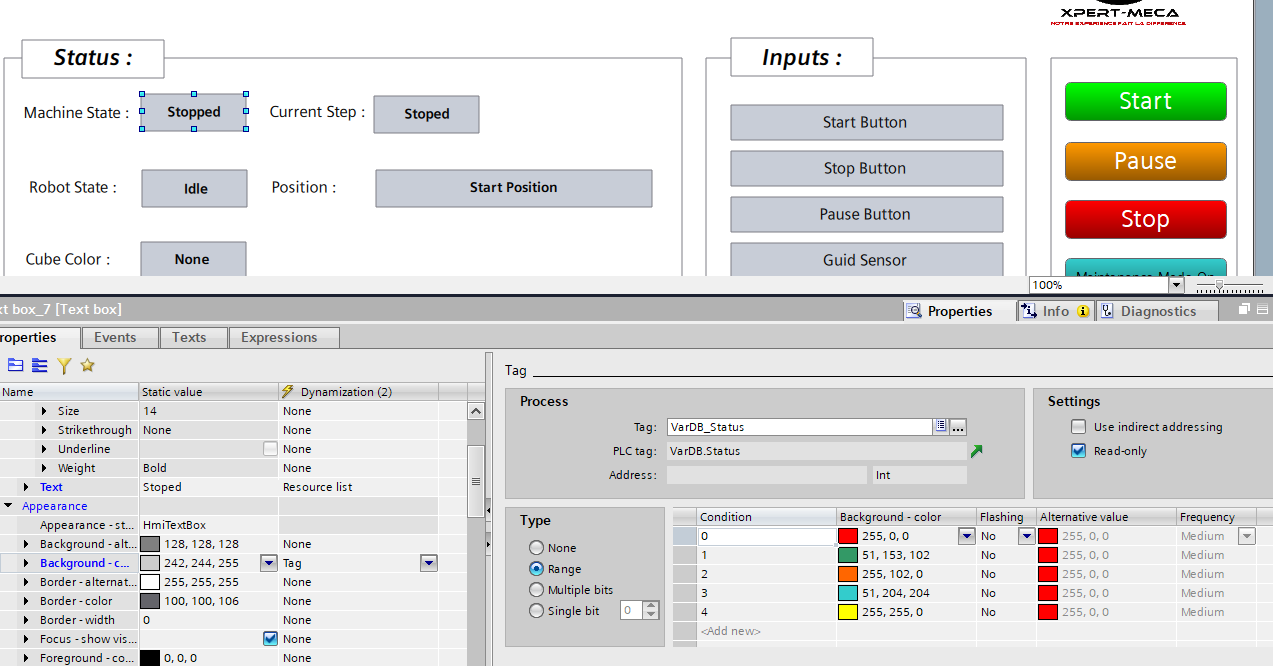
\includegraphics[width=1\textwidth]{Images/Chap3/_color.png}
    \caption{HMI configuration for changing an element's background color based on a variable's value.}
    \label{fig:status_color_config}
\end{figure}
\item Final Placement: Place the text box from the previous step on top of this graphic element. The result is a single status indicator that changes both its text and background color dynamically, as shown in Figure \ref{fig:status_color}.

\end{enumerate}

\begin{figure}[H]
    \centering
    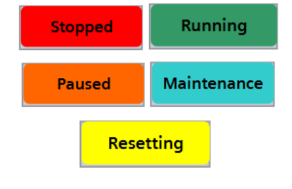
\includegraphics[width=0.5\textwidth]{Images/Chap3/state_boxes.png}
    \caption{Visual result of a status box with dynamic text and color.}
    \label{fig:status_color}
\end{figure}

\subsection{Dynamic Control and Button Interactivity}
The control buttons ("Start," "Stop," "Pause") are also configured to be interactive, preventing erroneous operations and enhancing safety. They are enabled or disabled based on the PLC’s status.

\begin{enumerate}
\item Add the Button: Place a button element on the HMI screen and give it a descriptive name like "Start\_Button."
\item Configure the Button's Event: In the button's properties, go to Events > Press. This is where you define the action the button will perform. For the "Start" button, the event uses a "SetTagValue" function to write the value 1 to the InputsDB\_StartBtn bit in the PLC, as shown in Figure \ref{fig:button_event}.
\begin{figure}[H]
\centering
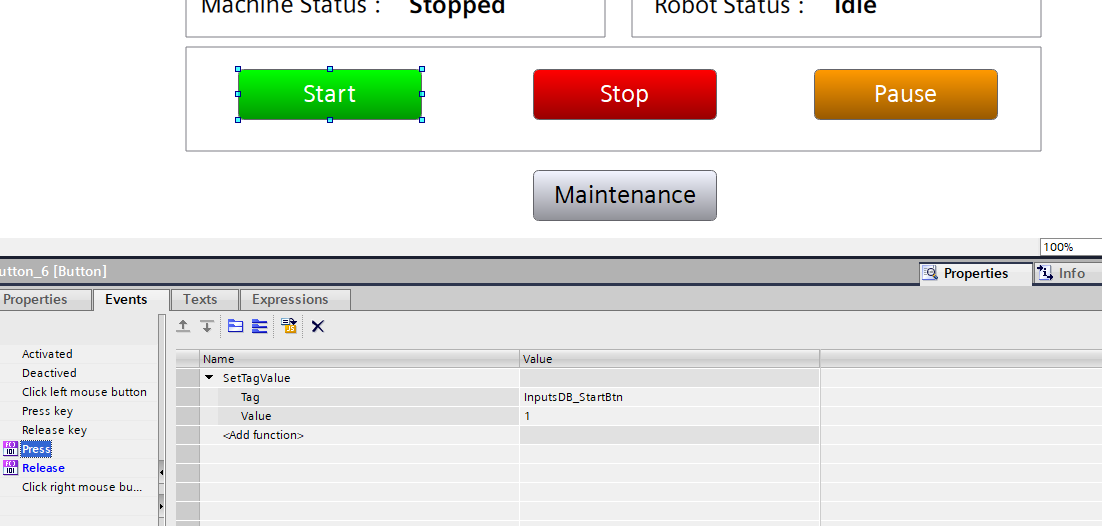
\includegraphics[width=1\textwidth]{Images/Chap3/_event.png}
\caption{HMI event configuration for a button press, which sets a PLC tag.}
\label{fig:button_event}
\end{figure}
\item Configure Button Operability: To control when the button can be pressed, navigate to the Properties of the button and go to General > Operability. Link this property to the PLC status tag (VarDB.MachineStatus). Then, configure the range so that the "Start" button is only operable when the MachineStatus tag is equal to 0 or 2 (the "STOPPED" or "PAUSED" state). This prevents the machine from being started while it is already running. The configuration is shown in Figure \ref{fig:button_operability_config}, and examples of multiple operability cases for buttons are shown in Figure \ref{fig:button_operability}.
\begin{figure}[H]
\centering
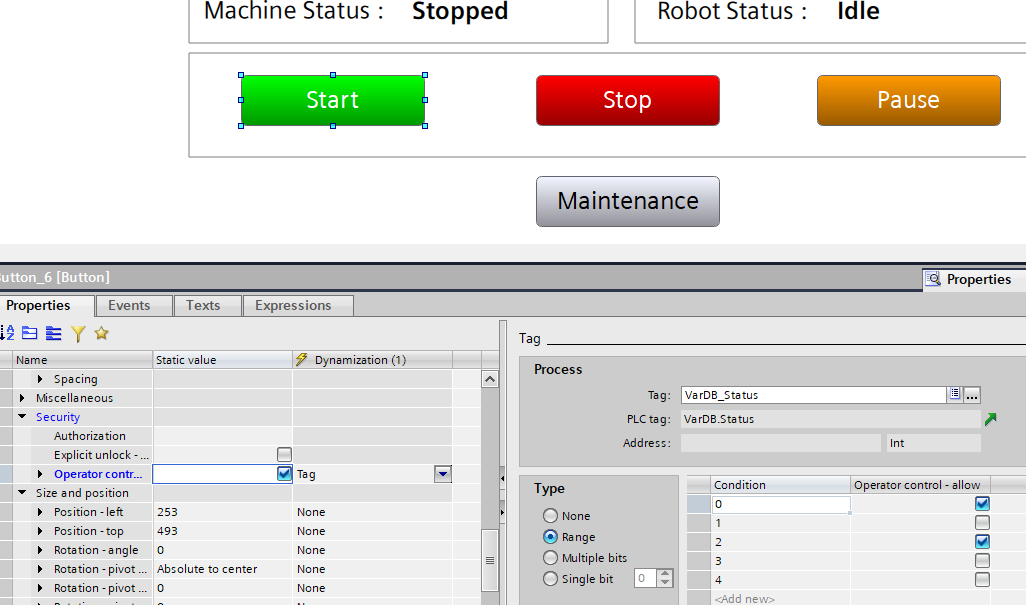
\includegraphics[width=0.8\textwidth]{Images/Chap3/_operability.png}
\caption{HMI configuration to link a button's operability to a PLC variable.}
\label{fig:button_operability_config}
\end{figure}
\end{enumerate}
\begin{figure}[H]
\centering
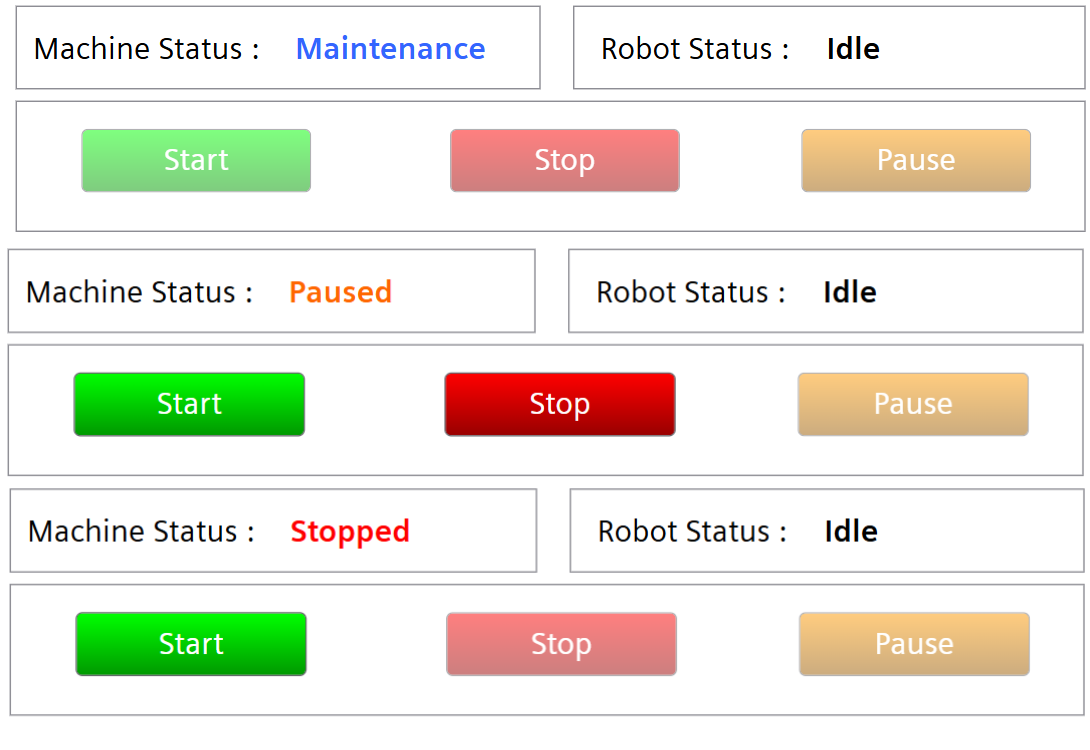
\includegraphics[width=0.6\textwidth]{Images/Chap3/MULTIPLECASES.png}
\caption{Examples of multiple operability cases for buttons.}
\label{fig:button_operability}
\end{figure}
\subsection{Real-time Value Displays (Counters)}
A critical function of the HMI is to provide real-time data to the operator, such as the count of sorted cubes.

\begin{enumerate}
\item Add a Display Field: Place an I/O field or a simple text box on the HMI screen.
\item Link to the PLC Tag: In the properties of the display field, navigate to General and link the Process value to the corresponding integer tag in the PLC (e.g., VarDB.RedCubesCounter), as shown in Figure \ref{fig:value_displays_config}.
\begin{figure}[H]
\centering
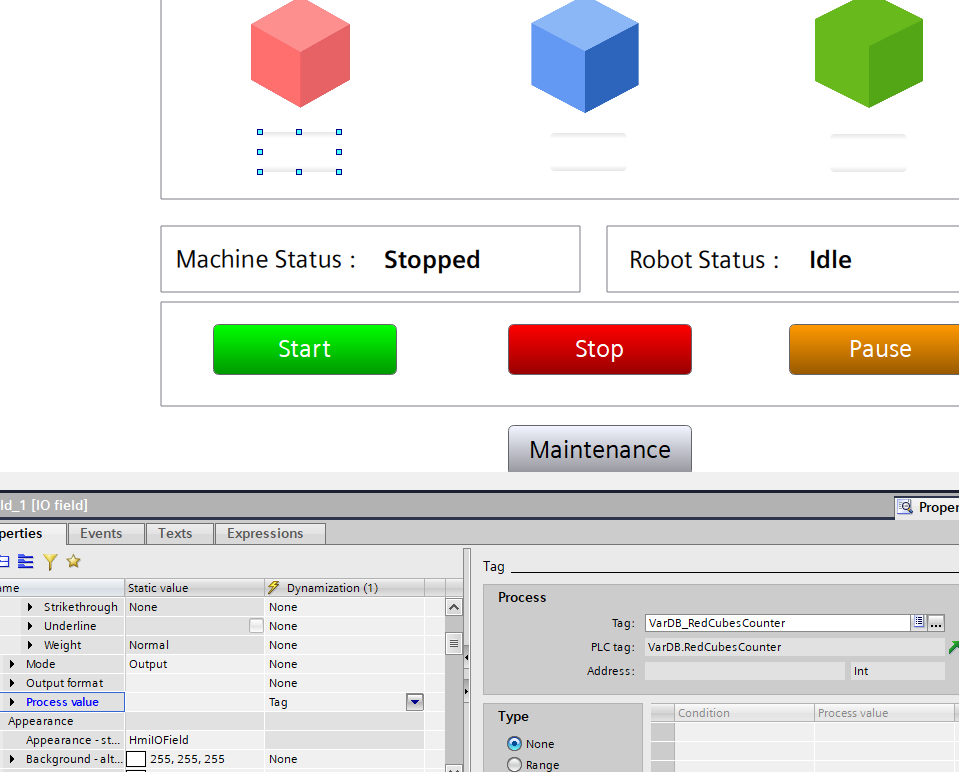
\includegraphics[width=0.8\textwidth]{Images/Chap3/value_displays.png}
\caption{HMI configuration for linking a display element to an integer tag in the PLC.}
\label{fig:value_displays_config}
\end{figure}
\item Format the Display: Configure the display format (e.g., number of decimal places, font, size) as needed. As the PLC tag's value increments, the number displayed on the HMI screen will update in real-time. The real-time display of cube counters on the HMI is shown in Figure \ref{fig:value_displays}.
\end{enumerate}
\begin{figure}[H]
\centering
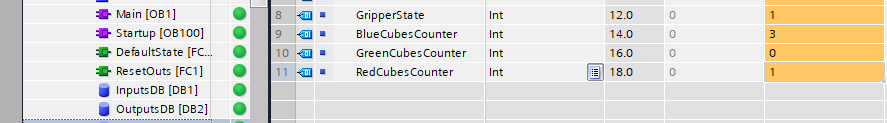
\includegraphics[width=0.8\textwidth]{Images/Chap3/cubecounters_vardb.png}
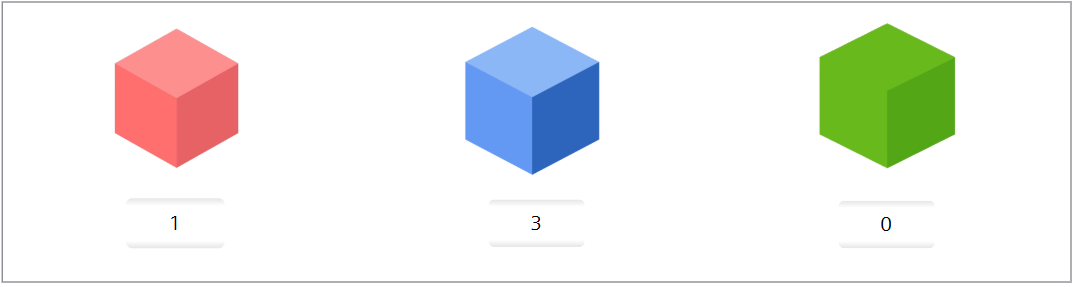
\includegraphics[width=0.8\textwidth]{Images/Chap3/cubecounters_hmi.png}
\caption{Real-time display of cube counters on the HMI.}
\label{fig:value_displays}
\end{figure}






\section{Conclusion}
The implementation of the control system for the robotic sorting cell, as detailed in this chapter, provides a comprehensive overview of the automation and human-machine interface development. We established a robust control philosophy centered on a Programmable Logic Controller (PLC) and utilized GRAFCET to meticulously design the sequential logic. While the complete, exhaustive programming of the automation and HMI is extensive, this chapter has presented the most critical and foundational steps. The provided logic blocks, programming principles, and design methods for elements like real-time counters and button operability are all that are necessary to construct the entire functional and structured control system. Crucially, the system's design also prioritizes the safety of the cell's operation and personnel, ensuring a secure and reliable sorting process. The structured approach outlined here is the cornerstone of a predictable, efficient, and safe robotic sorting solution.























\chapter{Integration and Simulation}

\section{Introduction}
This chapter details the final stages of the project, focusing on how all previously designed systems were integrated, validated through digital simulation, and prepared for future development. It moves beyond theoretical design to practical implementation, demonstrating the seamless communication between the core components and presenting a comprehensive outlook on potential improvements.

\section{System Integration and Interfacing}
The success of the automated sorting cell relies on the synchronized operation of its hardware and software components. This section explains the critical communication links and data exchange mechanisms established between the PLC, the robotic arm, the HMI, and a Raspberry Pi acting as an additional control and data hub.

\subsection{The Communication Framework}
The primary communication protocol used for this project was \textbf{PROFINET}. As a robust and high-speed industrial Ethernet variant, PROFINET enabled real-time data exchange, ensuring that all components operated in perfect harmony. The network architecture, as shown in Figure \ref{fig:communication_diagram}, utilizes a router as a centralized point of communication that allows the Raspberry Pi, the PLC, the HMI, and the KUKA robot controller to interface seamlessly. This setup provides network flexibility and scalability for the cell's communication.

\begin{figure}[H]
    \centering
    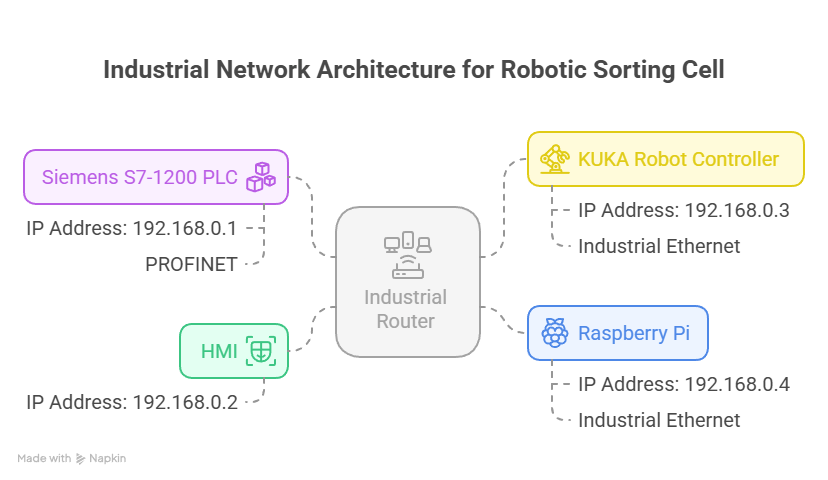
\includegraphics[width=0.8\textwidth]{Images/Chap4/communication_diagram.png}
    \caption{Communication diagram of the automated sorting cell.}
    \label{fig:communication_diagram}
\end{figure}

\subsection{Data Access via Python Scripting}
A crucial component of the system is the Raspberry Pi, which acts as a bridge between the vision system and the PLC. To facilitate this data exchange, a Python script was developed to communicate directly with the Siemens S7-1200 PLC. The script leverages a specialized library, such as \textbf{python-snap7}, an open-source Python wrapper for the Snap7 library, to establish a reliable TCP/IP connection to the PLC via the network router.

The script's primary function is to read from and write to the PLC’s dedicated \textbf{Data Blocks (DBs)}, which were pre-configured to store shared variables. Data is precisely addressed by its specific location within a DB, using the \textbf{DB number}, \textbf{byte offset}, and \textbf{bit offset}. This method is fundamental to the communication process, as it allows the script to directly manipulate variables in the PLC's memory.

For example, to read a variable, the Python script sends a command to the PLC specifying the DB number, the start byte, and the number of bytes to read. The PLC then sends the requested data back to the script. Conversely, to write a value, the script constructs a data packet containing the new value and the specific memory address, which the PLC then uses to update the corresponding variable.

This structured approach ensures that the Raspberry Pi can reliably provide the PLC with real-time data from the vision system, such as the CubeColor, thereby forming the core of the automated sorting logic. The ability to precisely read and write data at the byte level guarantees a robust and efficient communication link.

\begin{figure}[H]
    \centering
    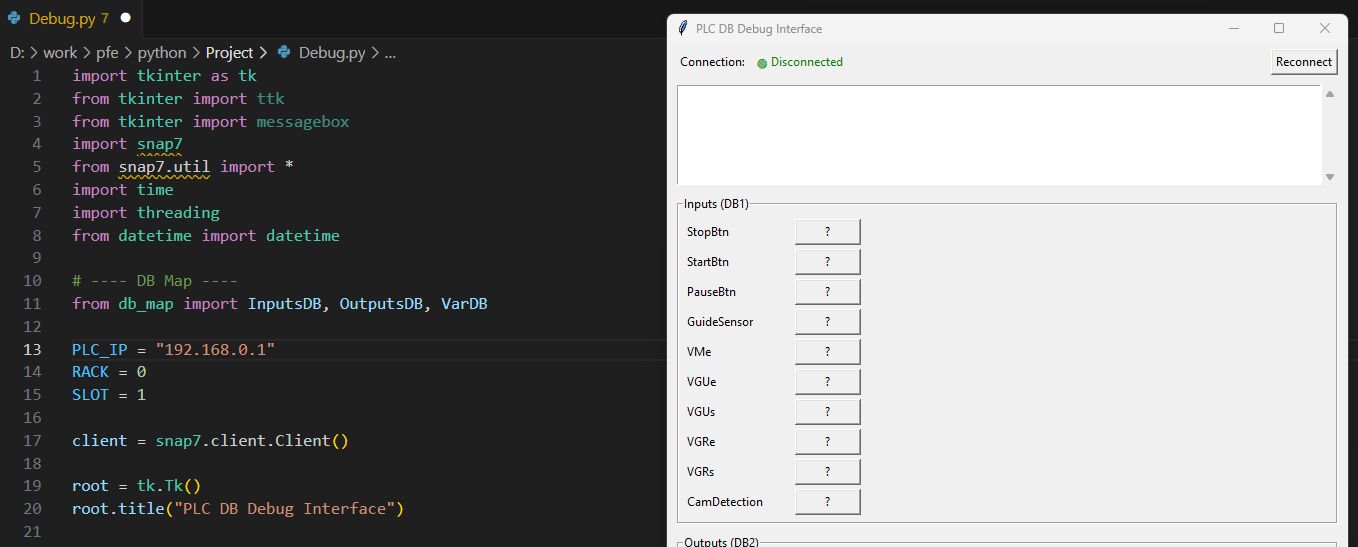
\includegraphics[width=1\textwidth]{Images/Chap4/python_interface.png}
    \caption{A Python-based interface for real-time PLC data access.}
    \label{fig:python_interface}
\end{figure}

\subsection{KUKA Robot Controller Interface}
The KUKA robotic arm's controller (KRC) is connected to the PLC via the PROFINET network and a central router. This network link allows the PLC to orchestrate the robot's movements by writing values to specific I/O addresses that are configured as shared data registers.

The robot's program is designed to continuously monitor these registers. For instance, the robot’s program looks for a change in the RobotPos variable. When the PLC writes a new value, the robot recognizes it as a command to move to a new position. After completing the move, the robot's program then writes a value to the RobotStatus register, informing the PLC that the task is complete and it is ready for the next command. This "read-then-write" mechanism is the foundation of the communication and coordination between the PLC and the robot.
\subsection{HMI Interface}
The HMI (Human-Machine Interface) is also connected to the router via PROFINET. It provides the operator with a graphical interface to interact with the system. The HMI's screens are linked to the PLC's variables, allowing it to:
\begin{itemize}
    \item \textbf{Display Real-Time Status:} Show the current state of the system, such as conveyor status, sensor feedback, and cube counts;
    \item \textbf{Receive Operator Commands:} Send commands to the PLC, such as START, STOP, or RESET, through on-screen buttons;
    \item \textbf{Monitor Alarms:} Display any system faults or warnings to the operator, enabling quick identification and resolution of issues.
\end{itemize}

\section{Digital Simulation and Verification}
Simulation was a cornerstone of this project, enabling comprehensive testing and validation of the entire system before physical implementation. This approach allowed for the early identification and resolution of potential issues, significantly reducing development time and minimizing risks. The simulation process was conducted across two distinct environments: the TIA Portal suite for automation logic and HMI, and a 3D modeling platform for physical and visual validation.

\subsection{TIA Portal Simulation}
The TIA Portal environment provides a powerful, integrated solution for simulating the entire control system before physical deployment. This process, often referred to as creating a \textbf{"digital twin" or "virtual commissioning"}, allows for a thorough, risk-free validation of the automation logic and network communication. The comprehensive simulation is carried out in a methodical, step-by-step manner.

First, the PLC's network settings are configured in the TIA Portal project. This includes assigning a specific IP address to the PROFINET interface of the virtual PLC. As shown in Figure \ref{fig:profinet_config}, the PLC is assigned the IP address \textbf{192.168.0.1}, which serves as its unique identifier on the network. This step is followed by compiling both the hardware configuration and the software to ensure there are no errors before the simulation begins.



The next critical step is to download the compiled program to the virtual PLC. The project is specifically downloaded to the \textbf{PLCSIM} instance, which acts as the simulated CPU. This ensures that the program is loaded into a virtual environment, allowing it to execute the control logic just as it would on a physical device. Once the download is complete, a connection is established between the TIA Portal engineering station and the virtual PLC, confirming that the simulation is online and ready for testing.
\begin{figure}[H]
    \centering
    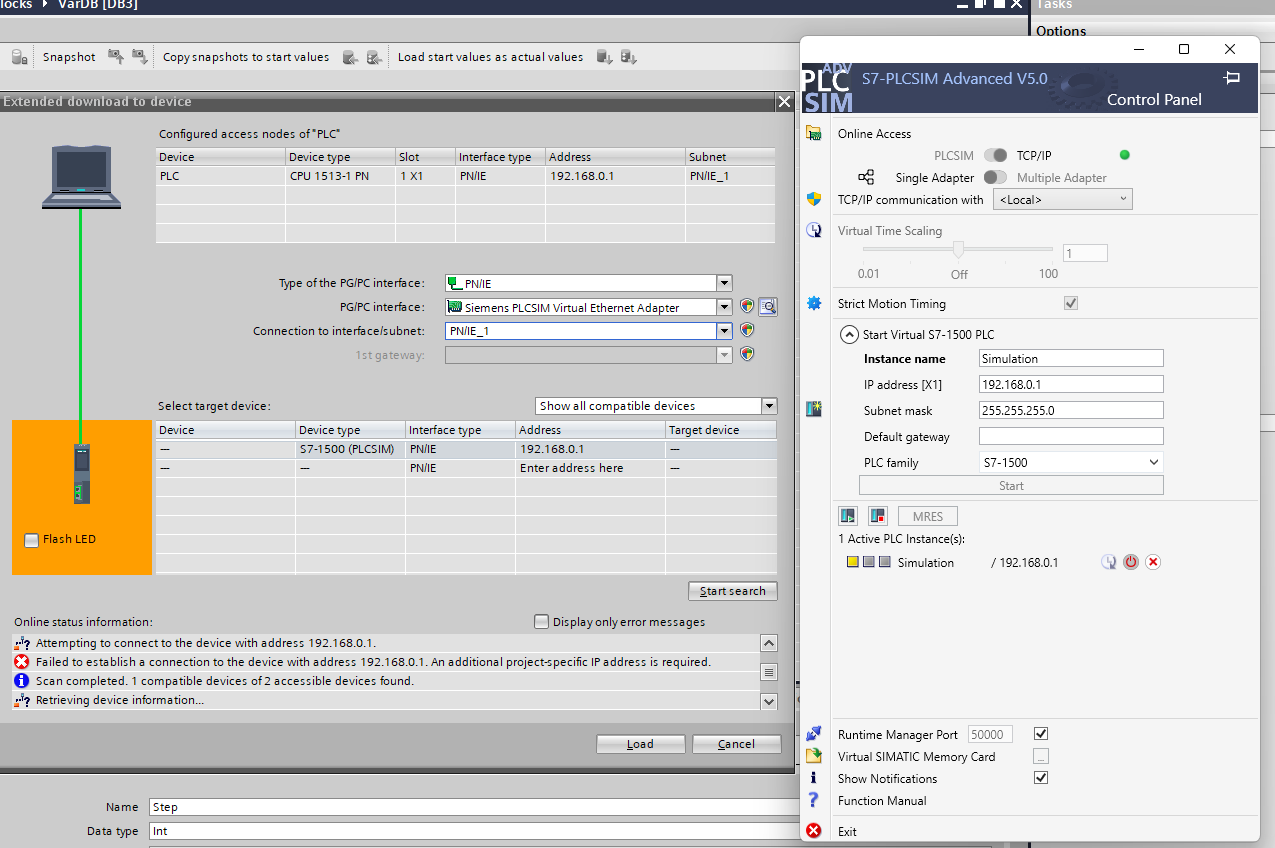
\includegraphics[width=0.9\textwidth]{Images/Chap4/PLC_PROFINET_Config.png}
    \caption{The PROFINET interface configuration to download the project in the simulated PLC.}
    \label{fig:profinet_config}
\end{figure}

With the PLC program running, the HMI can be simulated using \textbf{WinCC Unified}. TIA Portal automatically establishes a connection between the simulated HMI and the virtual PLC, allowing them to communicate in real time. This HMI can be accessed directly through a web browser, a key feature that allows for remote testing and validation of the user interface's operability. To access the interface, you first navigate to the specified IP address of the HMI in your browser, in this case, \textbf{192.168.0.2}. As the login page indicates, you must provide the correct user credentials to gain access to the control panel.

\begin{figure}[H]
    \centering
    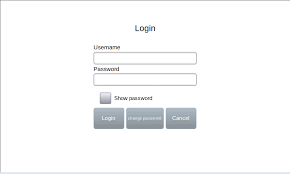
\includegraphics[width=0.6\textwidth]{Images/Chap4/HMI_Login_Page.png}
    \caption{The login page for the simulated HMI, accessible via a web browser.}
    \label{fig:hmi_login}
\end{figure}

Once logged in, the HMI provides a clear, visual interface with functional buttons and real-time data displays, enabling full interaction with the simulated system.

\begin{figure}[H]
    \centering
    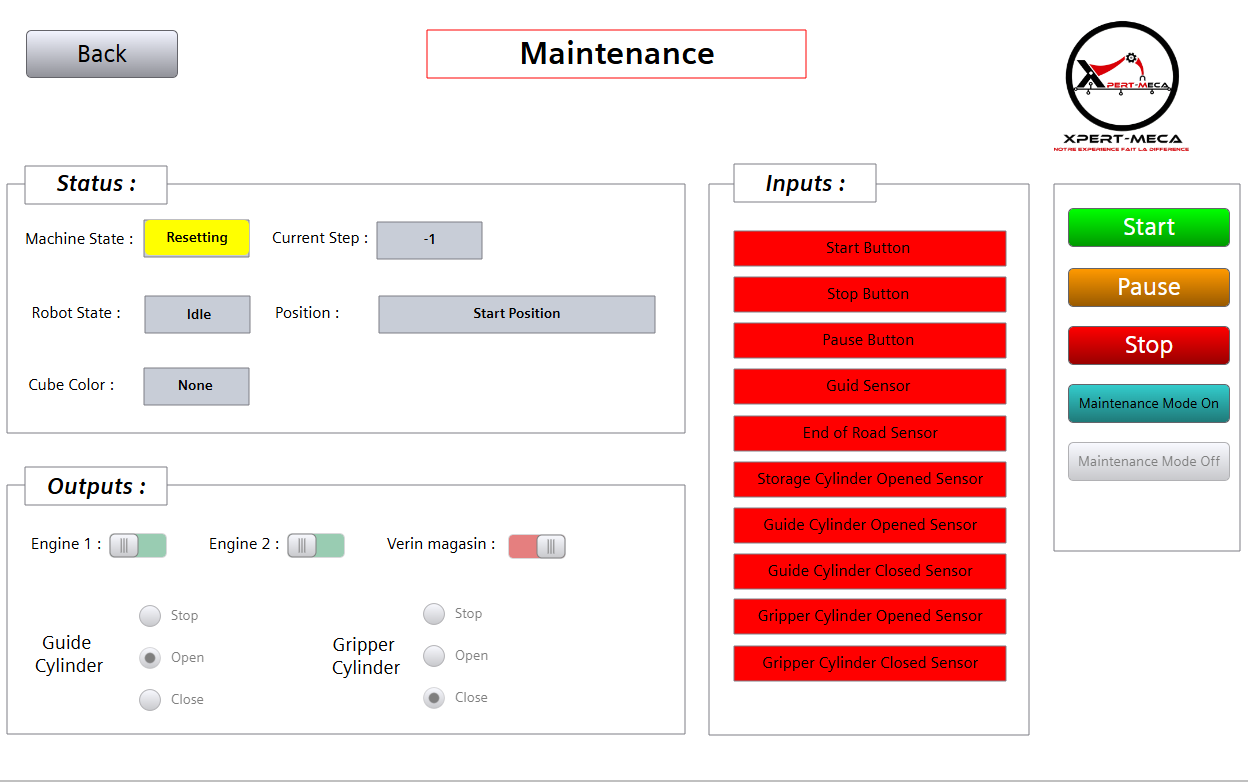
\includegraphics[width=0.8\textwidth]{Images/Chap4/HMI_Web_Simulation.png}
    \caption{The simulated HMI user interface with interactive elements.}
    \label{fig:hmi_web_simulation}
\end{figure}

To confirm the functionality of the system, all variables were monitored in real time. A crucial tool for this is the \textbf{Watch Table}, which provides a live view of the values of all internal tags and data blocks (DBs) on the virtual PLC. As seen in the watch table in Figure \ref{fig:watch_table}, variables like \textbf{`CubeColor`}, \textbf{`RobotPos`}, and \textbf{`RobotStatus` }update their values dynamically, proving that the control logic is executing correctly. This capability also allows for in-depth debugging by enabling a direct view into the logic, showing the status of each function block and its inputs and outputs, as demonstrated in Figure \ref{fig:online_diagnostics}.

\begin{figure}[H]
    \centering
    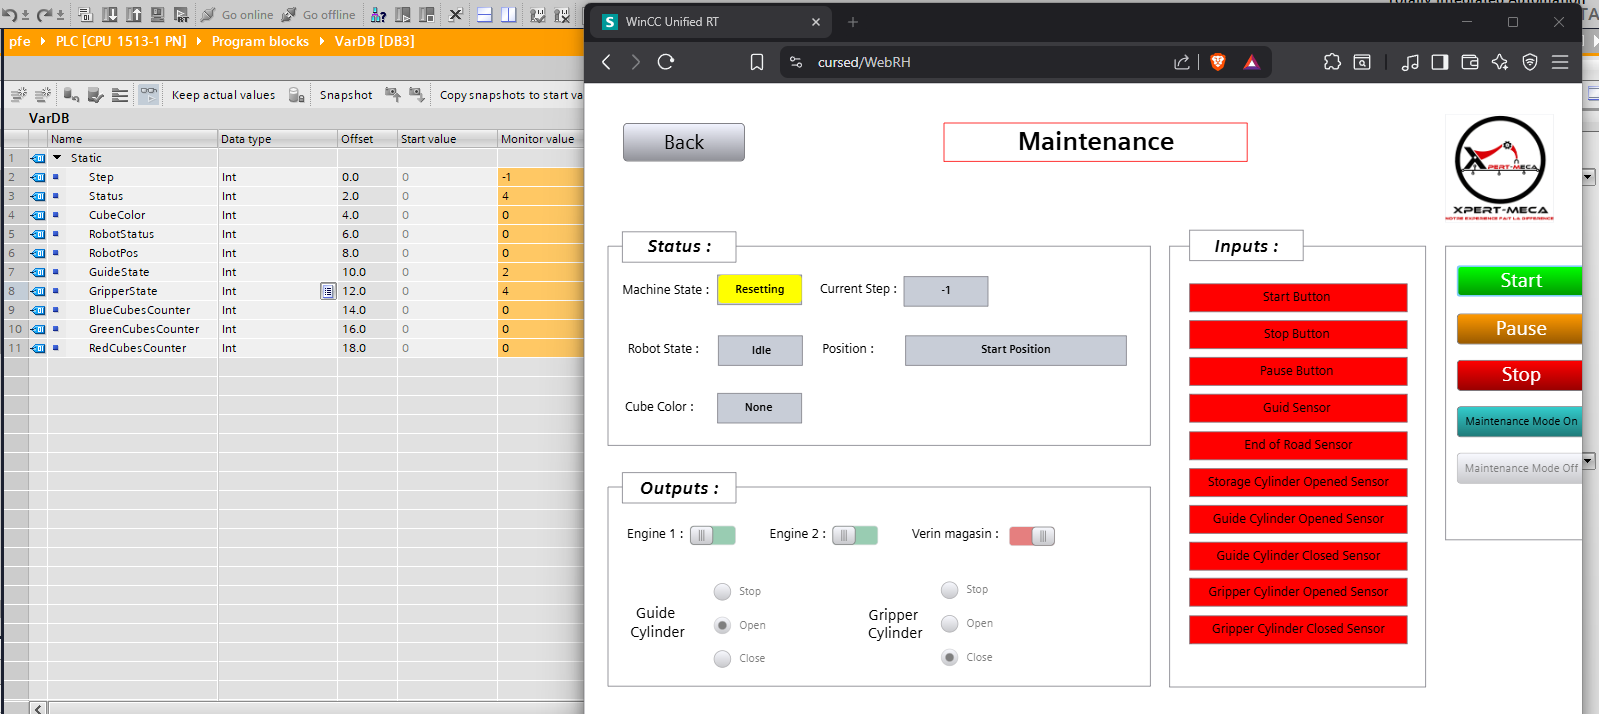
\includegraphics[width=1\textwidth]{Images/Chap4/Live_Watch_Table.png}
    \caption{The TIA Portal watch table, used to visualize and monitor real-time data from the PLC during simulation.}
    \label{fig:watch_table}
\end{figure}

\begin{figure}[H]
    \centering
    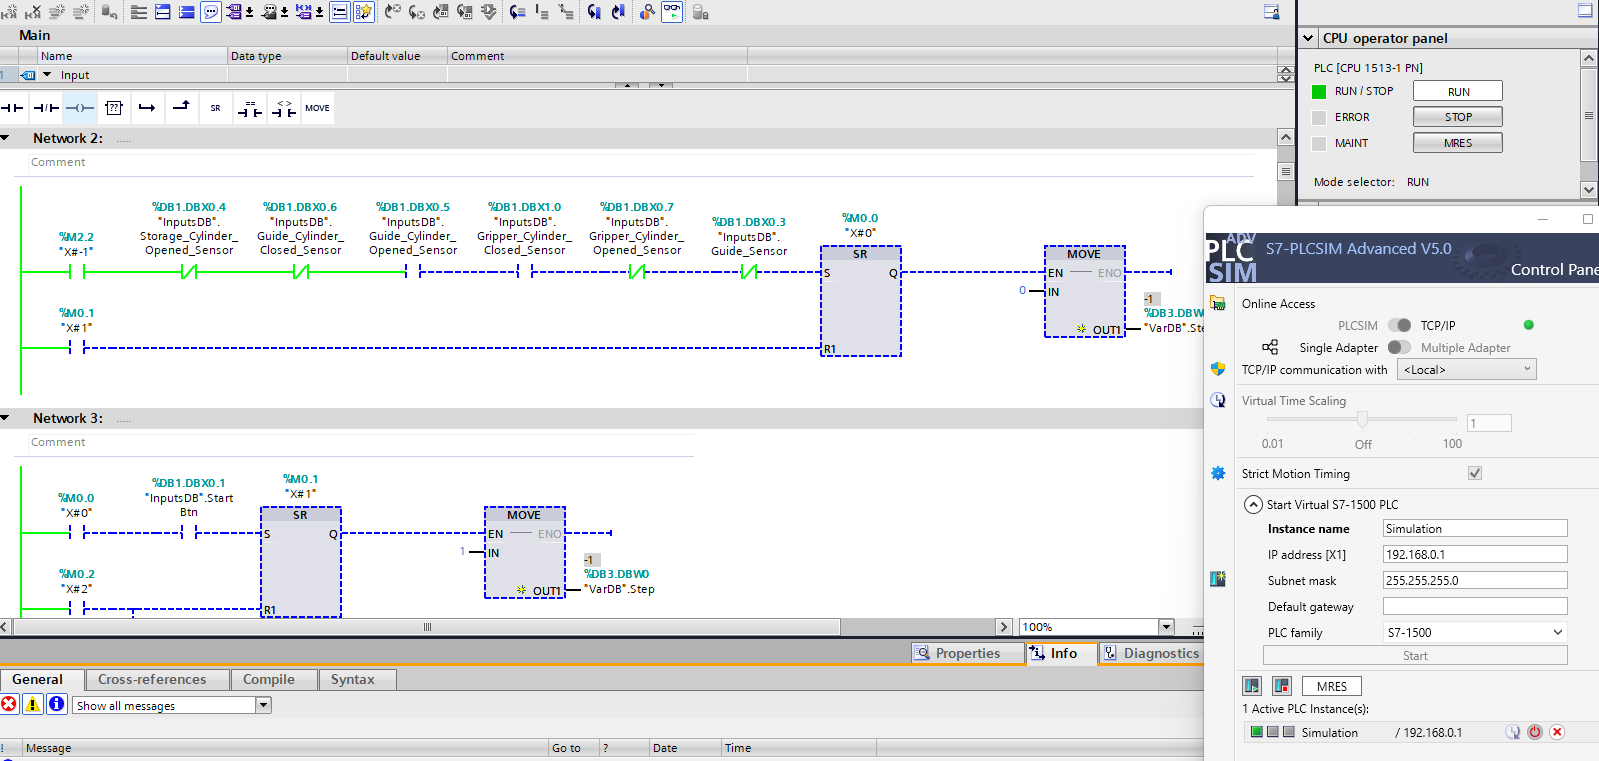
\includegraphics[width=1\textwidth]{Images/Chap4/Online_Diagnostics.png}
    \caption{Online diagnostics view of a function block, displaying the live values of its inputs and outputs.}
    \label{fig:online_diagnostics}
\end{figure}

\subsection{3D Simulation with Blender}
To create a realistic digital twin of the sorting cell, Blender was used to animate the system based on the control logic. The process involved several key steps:

\begin{itemize}
    \item \textbf{Model Optimization}: The original SolidWorks CAD models were imported into Blender. This process was critical, as the high-poly, detailed models were not suitable for a fluid animation workflow. To improve performance, the models were optimized by combining static parts (e.g., the frame and base) and reducing the overall number of components. This simplification made the project much more manageable and efficient for animation and rendering.
    
    \begin{figure}[H]
        \centering
        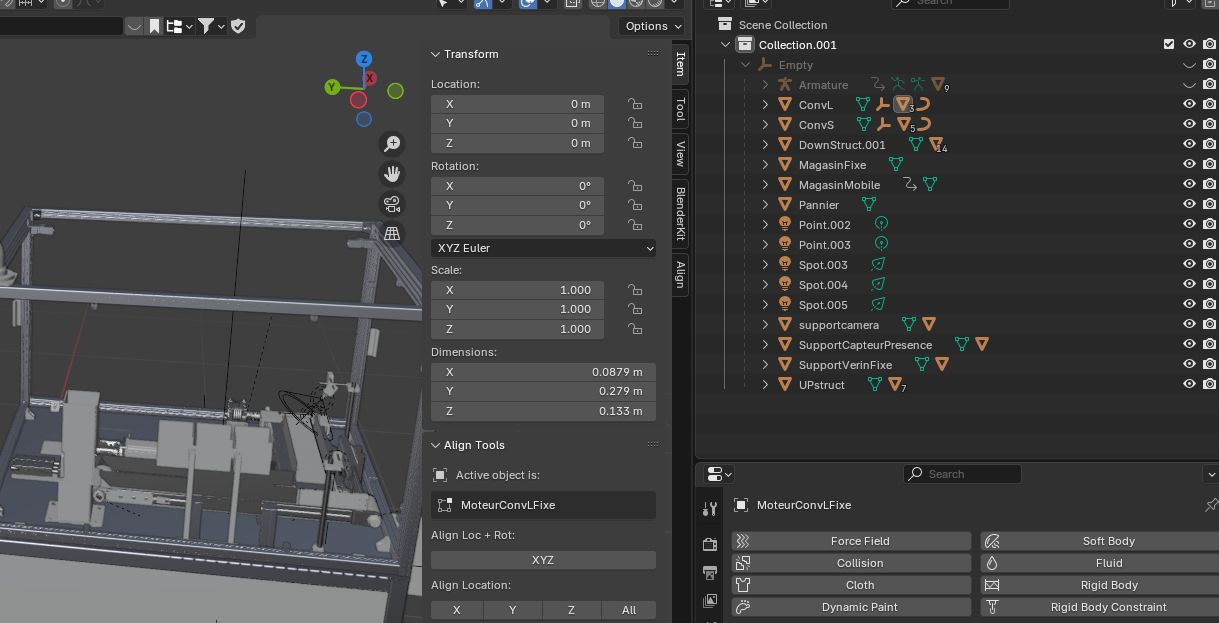
\includegraphics[width=0.9\textwidth]{Images/Chap4/Blender_Optimization.png}
        \caption{Blender collection parts}
        \label{fig:blender_optimization}
    \end{figure}
    
    \item \textbf{Texturing}: After optimization, realistic materials and textures were added to the models to visually represent the final appearance of the cell. As shown in Figure \ref{fig:blender_texturing}, this included applying appropriate colors and finishes to mimic painted metal, rubber, and other materials. This step was crucial for enhancing the visual fidelity of the simulation and creating a convincing representation of the physical cell.

    \begin{figure}[H]
        \centering
        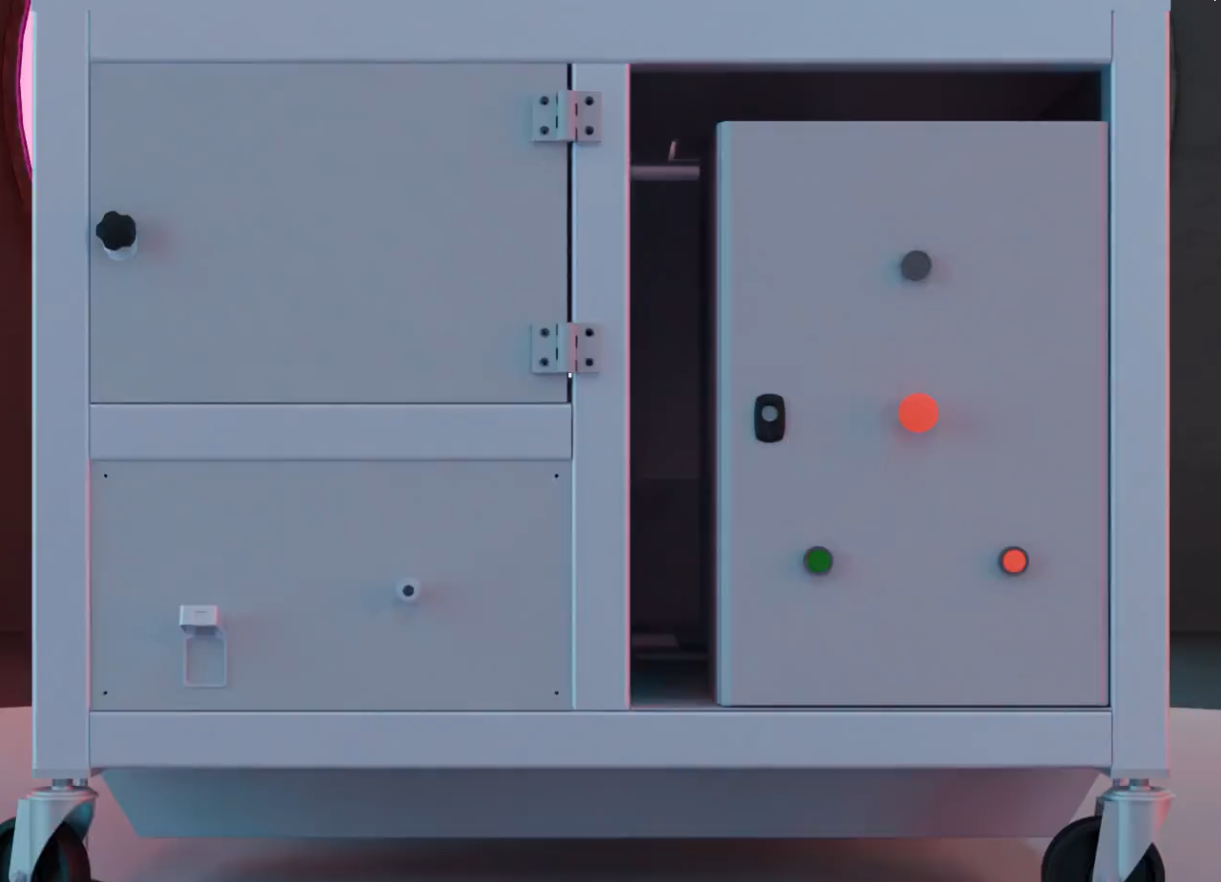
\includegraphics[width=0.6\textwidth]{Images/Chap4/Blender_Texturing.png}
        \caption{The 3D model in Blender with realistic materials and textures.}
        \label{fig:blender_texturing}
    \end{figure}

    \item \textbf{Physics and Rigging}: Physics simulations were applied to components that interact with the cubes, such as the conveyor belt and sorting mechanism, ensuring realistic behavior. This simulation was crucial for accurately depicting how the cubes would behave as they moved through the cell. Additionally, the robotic arm was \textbf{"rigged"} with a bone structure. This process of creating a digital skeleton allowed for the precise animation of the arm's joints and end-effector, ensuring that its movements accurately mimicked those controlled by the PLC. As seen in Figure \ref{fig:blender_rigging}, the rig provides a framework for animating the arm's complex movements.

    \begin{figure}[H]
        \centering
        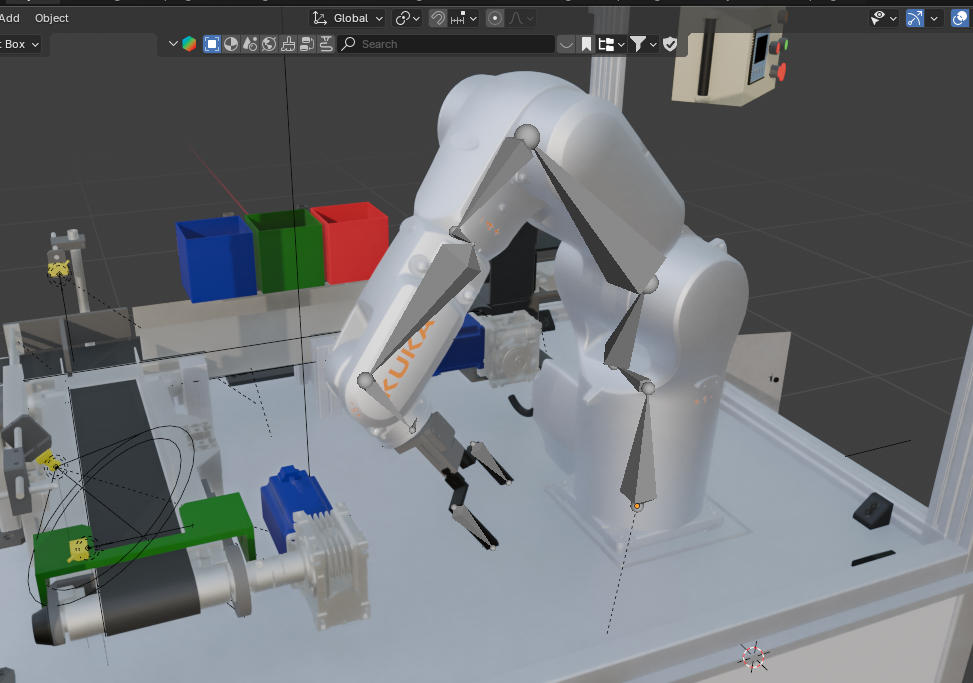
\includegraphics[width=0.6\textwidth]{Images/Chap4/Blender_Rigging.png}
        \caption{Robotic arm's bone structure.}
        \label{fig:blender_rigging}
    \end{figure}

    \item \textbf{Animation and Presentation}: The final step was to animate the complete sorting cycle from start to finish. This process involved synchronizing the rigged robotic arm and the physics-simulated cubes with the logical sequence defined in the PLC program. As demonstrated in Figure \ref{fig:blender_animation}, this detailed visual representation of the entire process served as a powerful tool for showcasing the project's functionality and for identifying any motion-related design flaws. The final rendered animation was used for both project verification and presentation purposes.

    \begin{figure}[H]
        \centering
        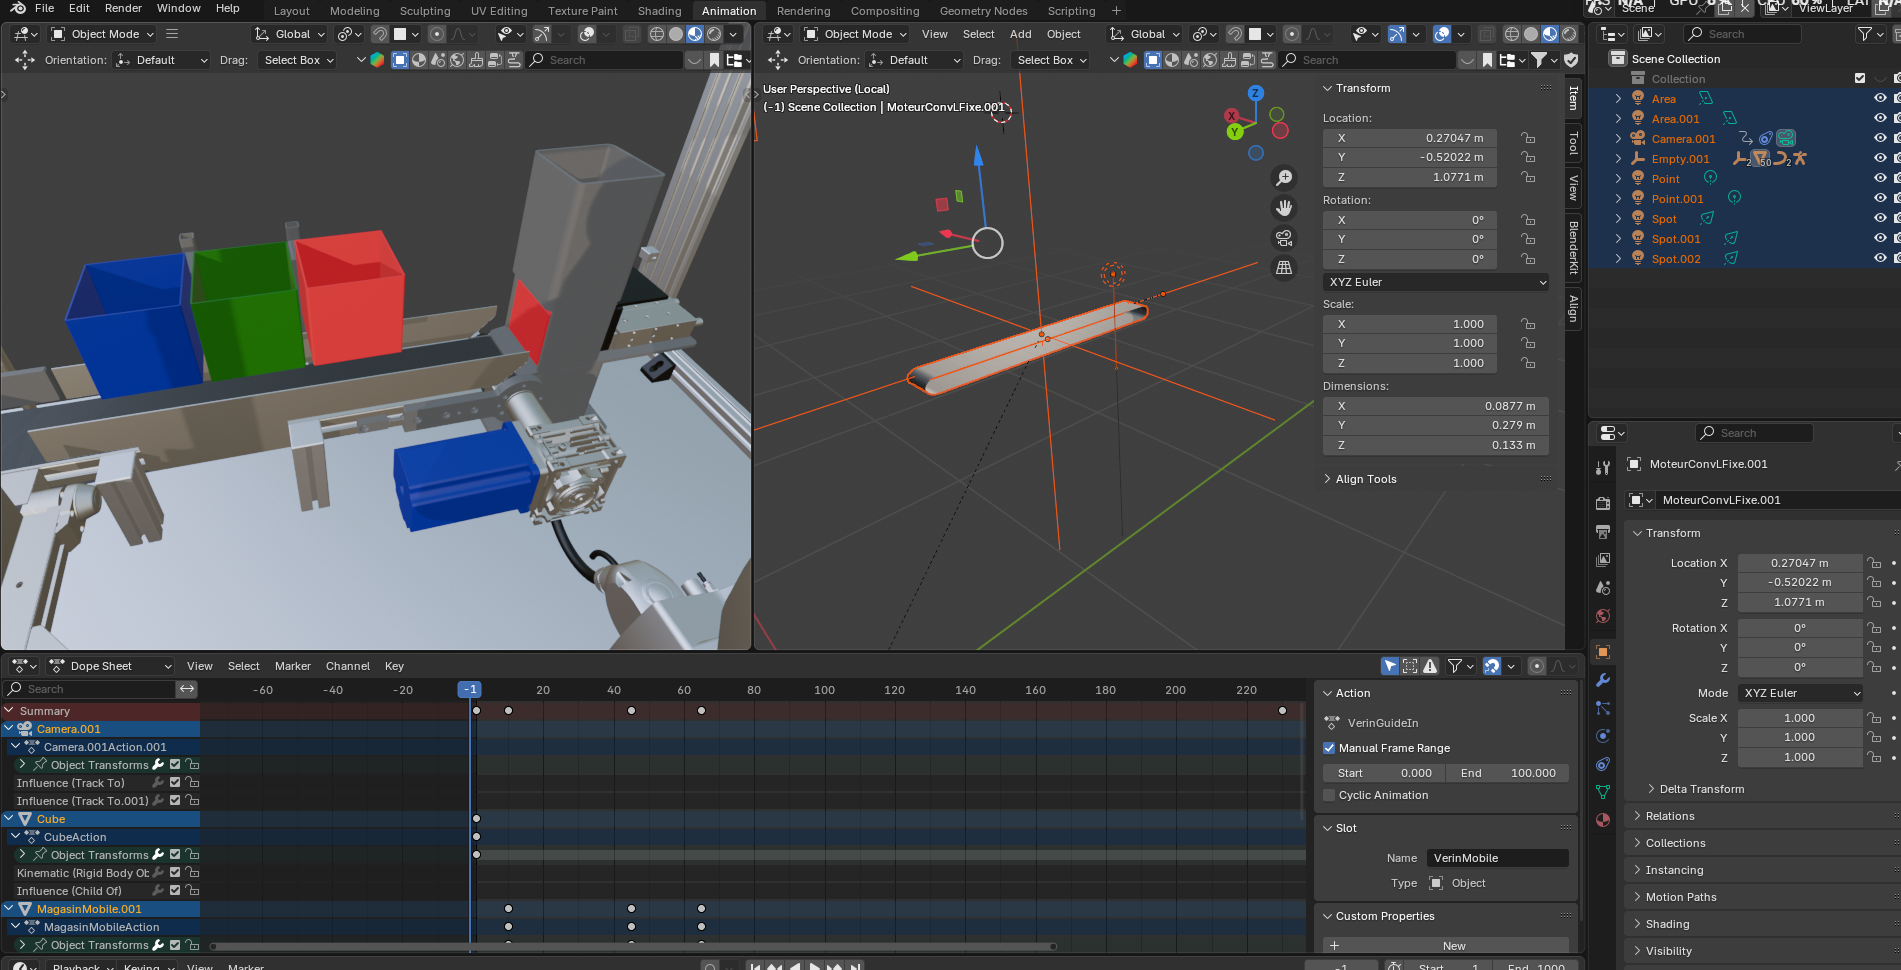
\includegraphics[width=1\textwidth]{Images/Chap4/Blender_Animation.png}
        \caption{Blender animation window and timeline}
        \label{fig:blender_animation}
    \end{figure}
\end{itemize}


\section{Conclusion}
This chapter successfully demonstrated the transition from theoretical design to a functional and verifiable system through advanced simulation. By meticulously detailing the PROFINET communication network, we established a clear link between the PLC, Raspberry Pi, and KUKA robot, highlighting the central role of a network router in orchestrating seamless data exchange. We then delved into the crucial process of virtual commissioning, showcasing how TIA Portal and Blender were used to create a comprehensive digital twin. This approach allowed for the rigorous testing of both the control logic and HMI functionality, as well as the accurate visualization of the cell's physical movements. The structured methodology presented here—from network configuration to real-time variable monitoring—is fundamental to the development of a predictable, efficient, and safe robotic sorting solution.

\begin{spacing}{1.3}
\chapter*{General Conclusion and Perspectives
%\markboth {Introduction }{}}
\markboth {General Conclusion and Perspectives}{}}
\addcontentsline{toc}{chapter}{General Conclusion and Perspectives}

\lettrine[lines=2]{T}\\his project successfully demonstrates the design and implementation of a functional and safe automated sorting cell, providing a complete framework from foundational concepts to a verifiable digital model. We began with a structured design approach, using GRAFCET to lay out a logical and sequential control strategy for the system's operation. This was followed by a detailed exploration of the hardware and software components, including the PLC, robotic arm, and vision system, and their comprehensive integration via a PROFINET network.

The project's success was significantly underpinned by the use of virtual commissioning, a process that allowed for the thorough simulation and debugging of the entire system. By creating a digital twin in software environments like TIA Portal and Blender, we were able to test the control logic, HMI, and physical mechanics in a risk-free environment, which is an invaluable step in modern industrial automation.

While the comprehensive programming of the system is extensive, this document has presented the core principles, logical framework, and critical design elements necessary to build the entire functional control system. The detailed methodology and the focus on safety, as highlighted throughout the project, serve as a cornerstone for future applications. The work not only proves the feasibility of the proposed design but also provides a robust and repeatable process for the development of similar automated solutions.

Building upon these achievements, several key areas for future improvement and development have been identified. These enhancements could further optimize the system's performance, expand its capabilities, and increase its value in a real-world industrial setting.

\begin{itemize}
\item \textbf{Advanced Sorting Algorithms}: The current system sorts by color. Future work could integrate more advanced sorting criteria, such as shape or weight detection, by adding a 3D vision system or a weighing scale to the conveyor line;

\item \textbf{Production Integration}: The cell could be integrated into a wider manufacturing environment by linking the PLC to a Manufacturing Execution System (MES). This would enable production scheduling, material tracking, and overall performance monitoring;

\item \textbf{Predictive Maintenance}: By collecting and analyzing data on motor runtimes, cycle counts, and sensor performance, the system could be upgraded with a predictive maintenance module. This would allow for the proactive scheduling of maintenance tasks, minimizing downtime and extending the lifespan of the equipment;

\item \textbf{Enhanced Simulation Fidelity}: While Blender provided an effective platform for visual simulation, integrating the digital twin with a more powerful game engine like \textbf{Unreal Engine} could dramatically increase the realism of the simulation. This would allow for more accurate physics, lighting, and a higher level of graphical detail, providing an even more immersive and precise virtual testing environment;

\item \textbf{Network and System Security}: With the increasing interconnectedness of industrial systems, a crucial area for future development is security. This would involve implementing measures to protect the control network from unauthorized access and cyber threats. Potential improvements include network segmentation, firewalls, and user authentication protocols to ensure the integrity and reliability of the automation cell.
\end{itemize}

\end{spacing}
\newpage

\addcontentsline{toc}{chapter}{Bibliography} % Adds "Bibliography" to the Table of Contents
\begin{thebibliography}{99}
\label{sec:bibliography}
\bibitem{Xpert_Meca_Contact_Page}
\textbf{Xpert-Meca}. \textit{Contact Page}. Available at: \url{https://www.xpert-meca.com/en/contactus}.

\bibitem{OBG_Website}
\textbf{OBG}. \textit{Website}. Available at: \url{https://www.obg.tn/ar}.

\bibitem{FANUC_Exmpl}
\textbf{Saenz, A.} \textit{Super Fast FANUC Robot Sorts Candy According to Color}. SingularityHub. Available at: \url{https://singularityhub.com/2010/12/01/super-fast-fanuc-robot-sorts-candy-according-to-color-video/}.

\bibitem{ABB_Exmpl}
\textbf{ABB}. \textit{ABB demonstrates the IRB 360 FlexPicker}. Cadenas. Available at: \url{https://partsolutions.com/abb-robotics-transform-peperami-packaging-line-into-snack-sausage-ballet/}.

\bibitem{ZenRobotics_Exmpl}
\textbf{ZenRobotics}. \textit{ZenRobotics Recycler Overview}. Cadenas. Available at: \url{https://www.terex.com/zenrobotics/}.

\bibitem{TIA_Portal_Manual}
\textbf{Siemens}. \textit{TIA Portal V18: System Manual}. Available at: \url{https://sieportal.siemens.com/en-ww/search?scope=knowledgebase&Type=siePortal&SearchTerm=&SortingOption=CreationDateDesc&EntryTypes=all&Page=0&PageSize=20&ProductNodePath=%2F13613%2F24841%2F14666%2F14667%2F14672%2F14673%2F}.

\bibitem{Blender_Manual}
\textbf{Blender Foundation}. \textit{Blender Manual}. Available at: \url{https://docs.blender.org/manual/en/latest/}.

\bibitem{Python_docs}
\textbf{Python Software Foundation}. \textit{Python 3.13.7 Documentation}. Available at: \url{https://docs.python.org/3/}.

\bibitem{OpenCV_docs}
\textbf{OpenCV}. \textit{OpenCV Documentation}. Available at: \url{https://docs.opencv.org/4.x/}.

\end{thebibliography}

\vspace{1em} % Adds a small vertical space before the final phrase
\noindent Accessed during the months of May, June, July and august 2025.
\newpage
\addcontentsline{toc}{chapter}{Annexes}
\section*{\Huge Annexes}
\setcounter{figure}{0}
\renewcommand{\thefigure}{A.\arabic{figure}}
\pagestyle{plain}

\begin{figure}[H]
\centering
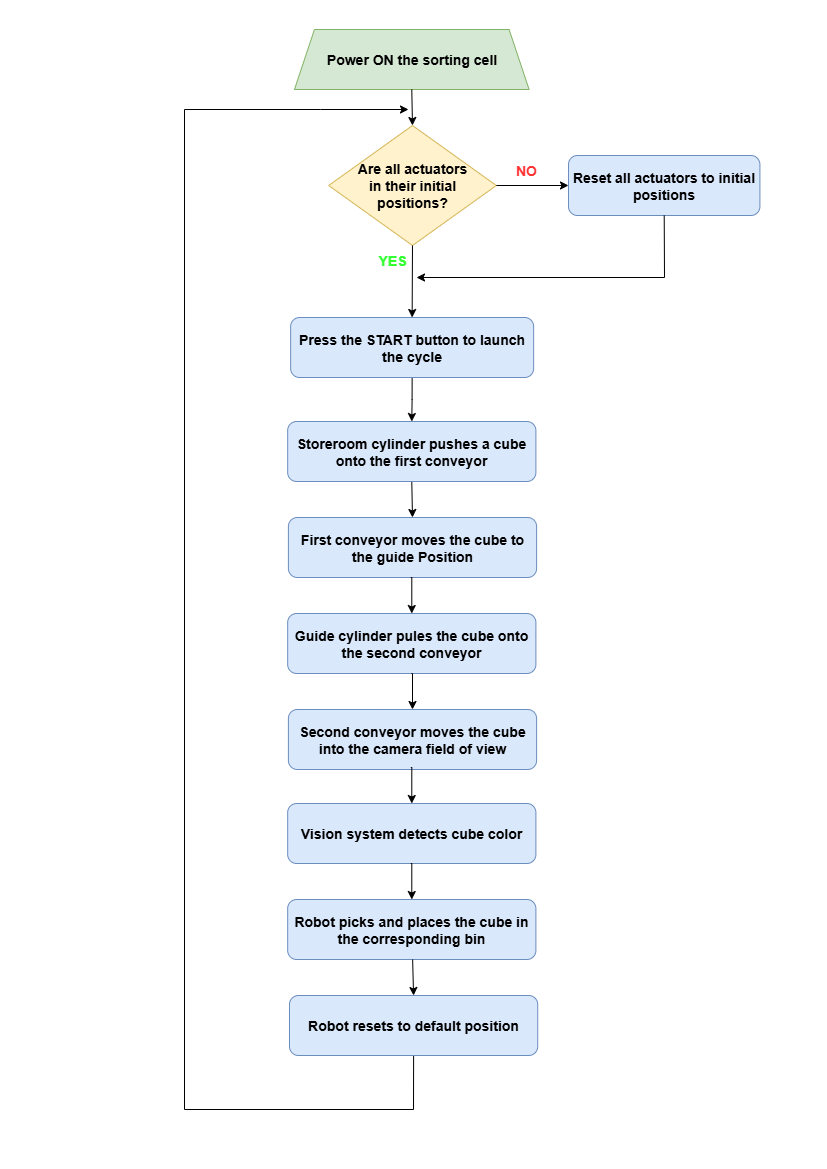
\includegraphics[width=0.9\textwidth]{Images/Chap2/Flowchart.drawio.png}
\caption[General System Flowchart]{General System Flowchart}
\label{fig:Flowchart}
\end{figure}


\begin{figure}[H]
\centering
 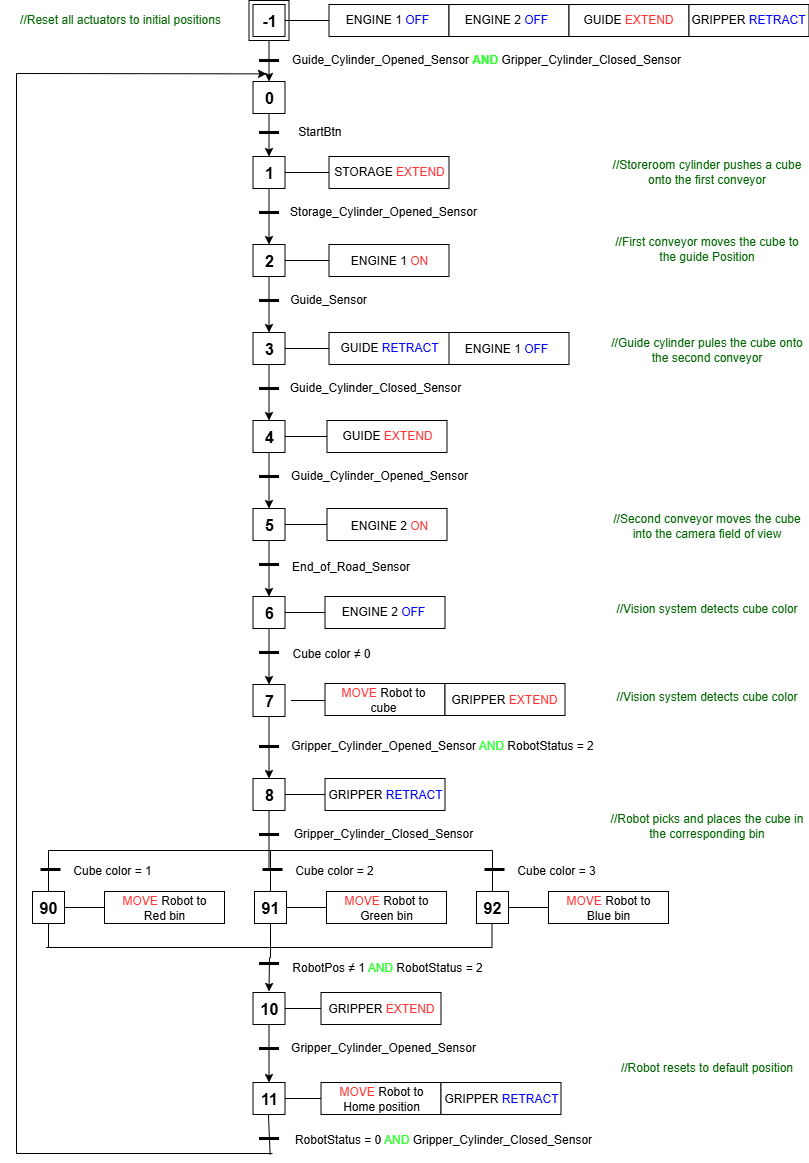
\includegraphics[width=1\textwidth]{Images/Chap3/graphcet.png}
\caption{GRAFCET of the sorting cell's control logic.}
\label{fig:grafcet_logic}
\end{figure}


\begin{figure}[H]
\centering
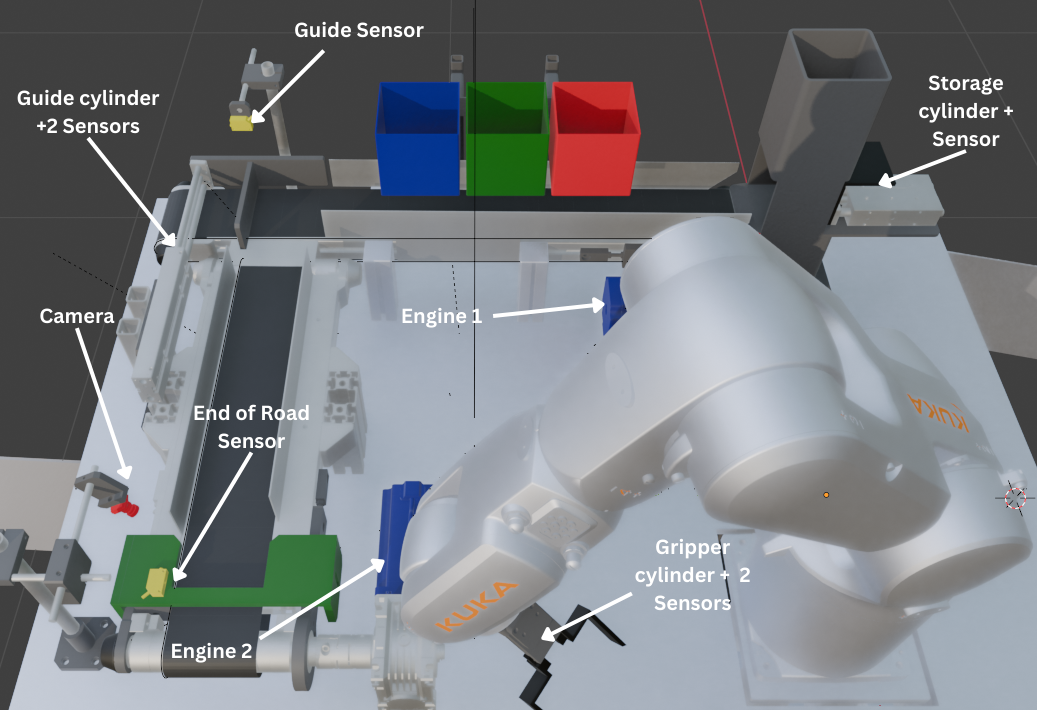
\includegraphics[width=0.9\textwidth]{Images/Chap3/cell_3d_view_annotated.png}
\caption{3D representation of the automated sorting cell with key components.}
\label{fig:cell_3d_view_annotated}
\end{figure}

\begin{figure}[H]
    \centering
    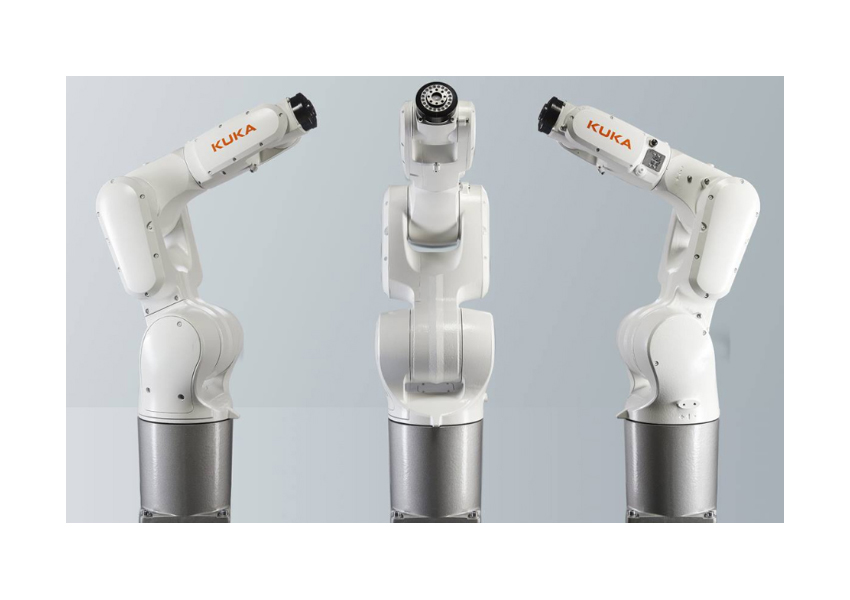
\includegraphics[width=0.9\textwidth]{Images/Chap2/kukarobot.jpg}
    \caption[ KUKA KR AGILUS Robot]{KUKA KR AGILUS Robot}
    \label{fig:KukaRobot}
\end{figure}

\begin{figure}[H]
    \centering
    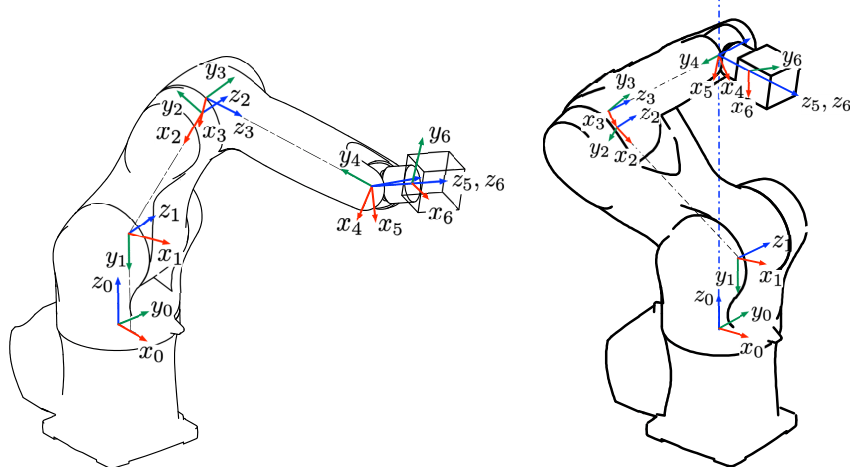
\includegraphics[width=0.8\textwidth]{Images/Chap2/kukaAxis.png}
    \caption[ Six-Axis Configuration]{Six-Axis Configuration}
    \label{fig:KukaAxis}
\end{figure}

\begin{figure}[H]
\centering
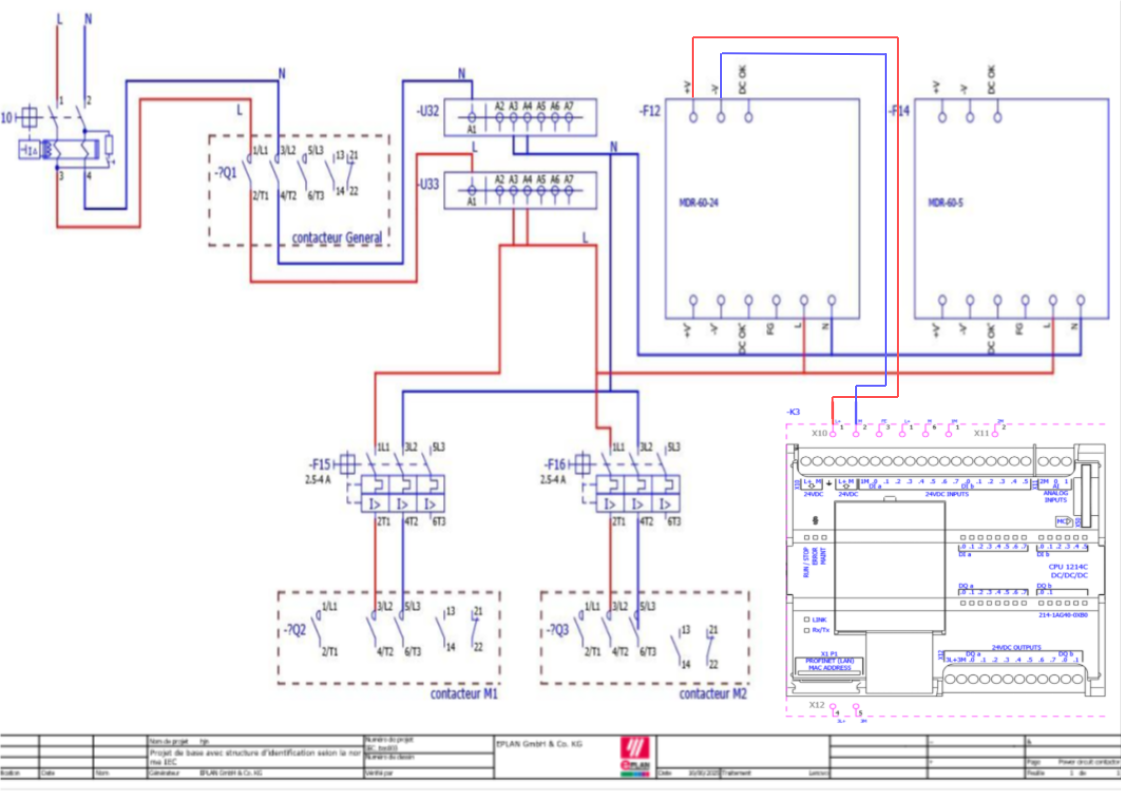
\includegraphics[width=1\textwidth]{Images/Chap2/elecCabinetSchema.png} 
\caption[Electrical Wiring Diagram]{Electrical Wiring Diagram}
\label{fig:electrical_diagram}
\end{figure}

\begin{figure}[H]
    \centering
    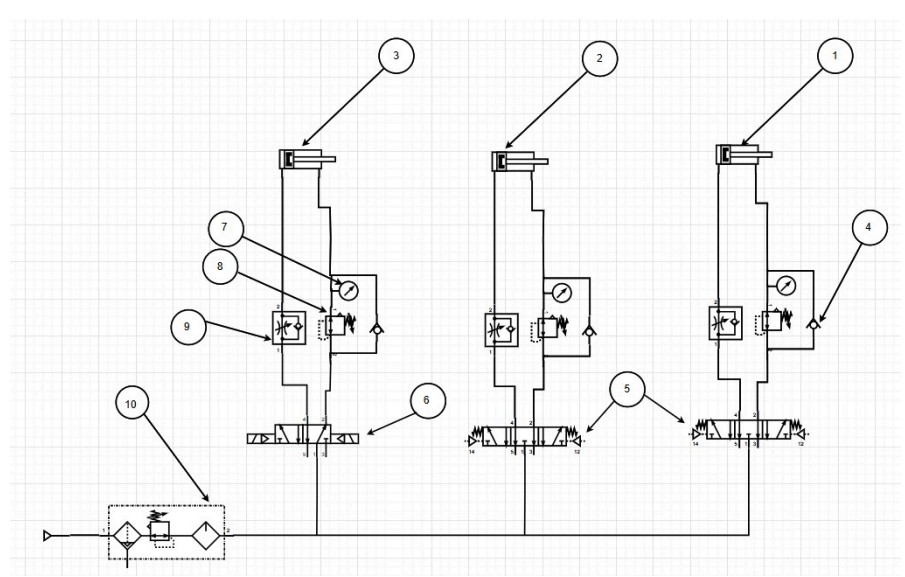
\includegraphics[width=1\textwidth]{Images/Chap2/pneuCabDiag.jpg} % Path for the pneumatic diagram
    \caption[Pneumatic Wiring Diagram]{Pneumatic wiring diagram of the automated system.}
    \label{fig:pneumatic_diagram}
\end{figure}



\begin{figure}[H]
\centering
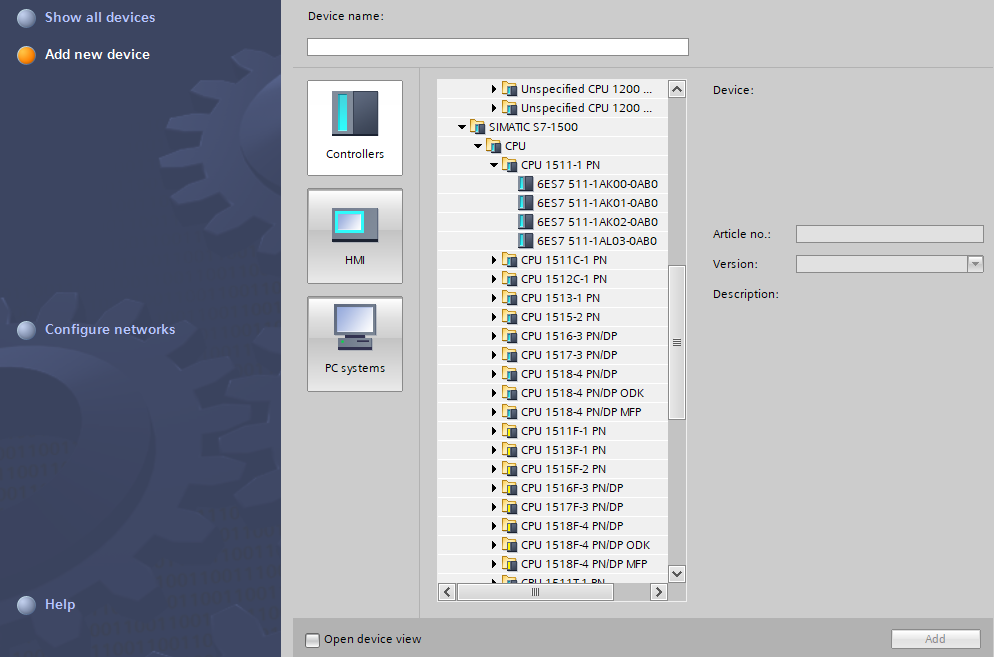
\includegraphics[width=0.8\textwidth]{Images/Chap3/PLCselection.png}
\caption{Hardware selection for the PLC.}
\label{fig:plc_selection}
\end{figure}

\begin{figure}[H]
\centering
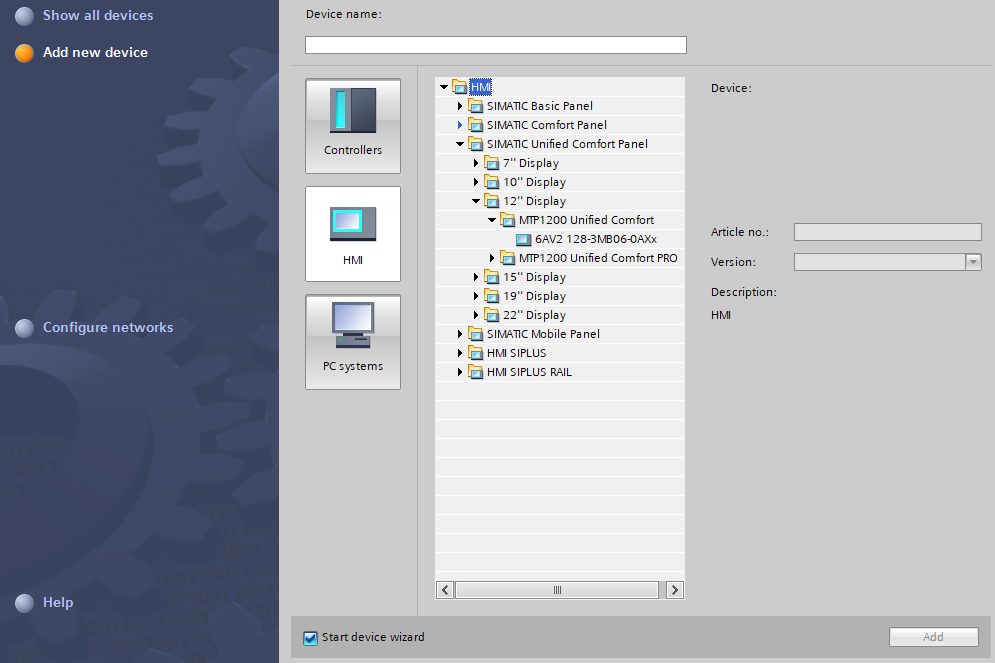
\includegraphics[width=0.8\textwidth]{Images/Chap3/HMIselection.png}
\caption{Hardware selection for the HMI panel.}
\label{fig:hmi_selection}
\end{figure}

\begin{figure}[H]
\centering
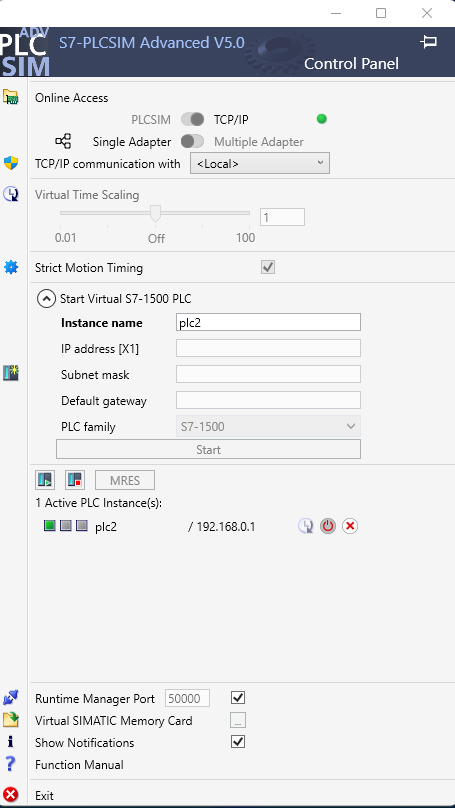
\includegraphics[width=0.4\textwidth]{Images/Chap2/PLCSIM_workspace.png}
\caption{S7-PLCSIM Advanced Workspace for virtual commissioning.}
\label{fig:PLCSIM_workspace}
\end{figure}

\begin{figure}[H]
\centering
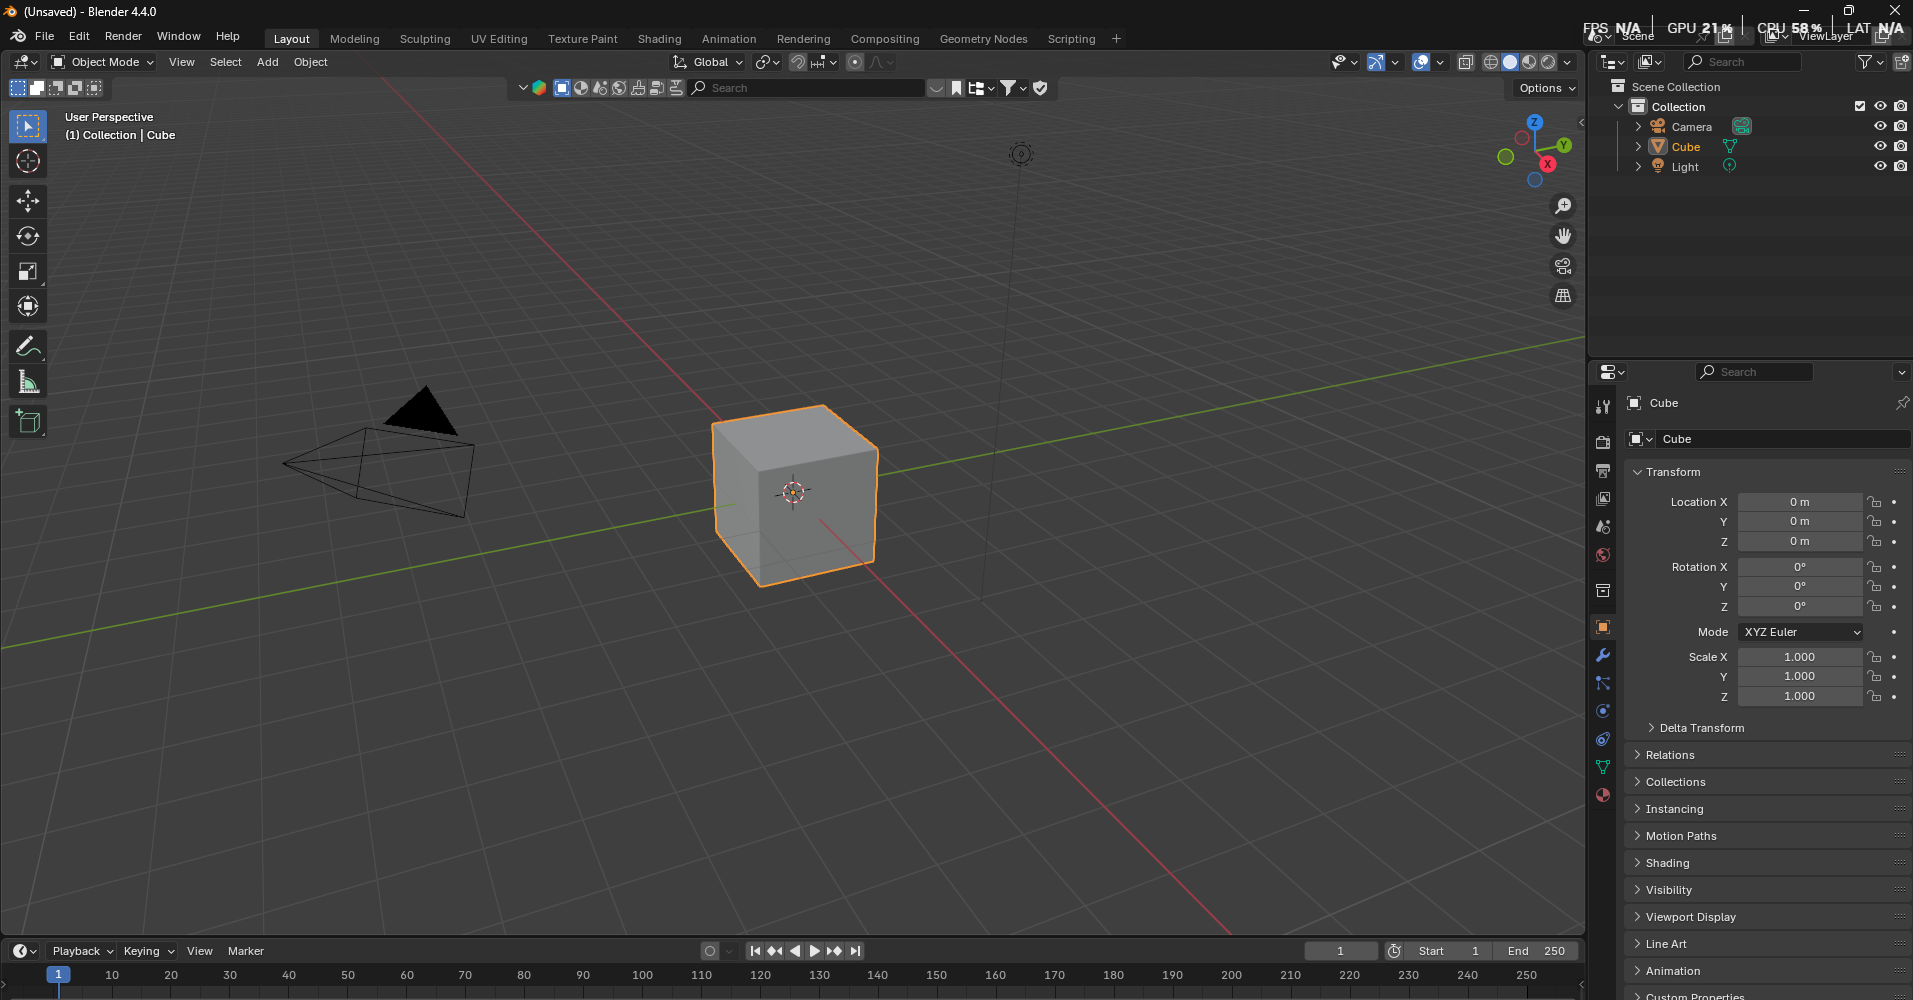
\includegraphics[width=1\textwidth]{Images/Chap2/Blender_workspace.png}
\caption{Blender Workspace.}
\label{fig:Blender_workspace}
\end{figure}

\begin{figure}[H]
\centering
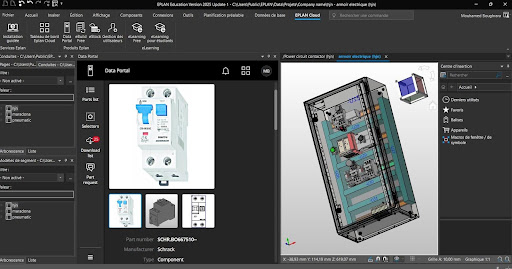
\includegraphics[width=1\textwidth]{Images/Chap2/EPLAN_workspace1.jpg}
\end{figure}




\begin{figure}[H]
\centering
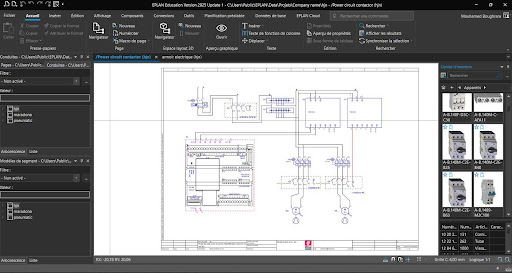
\includegraphics[width=1\textwidth]{Images/Chap2/EPLAN_workspace2.jpg}
\caption{EPLAN Workspace.}
\label{fig:EPLAN_workspace}
\end{figure}
% These commands ensure the bibliography is on a new page and added to the ToC.
\cleardoublepage % Ensures bibliography starts on a right-hand page for 'book' and 'report'
\phantomsection % Provides an anchor for hyperref to link to this page

\end{document}

